% --------------------------------------------------
% DOCUMENT CLASS
% --------------------------------------------------

\documentclass[../thesis.tex]{subfiles}

\begin{document}

\newpage

% --------------------------------------------------
% NEW KEYNESIAN MODEL
% --------------------------------------------------

\subsection{Regional New Keynesian Model}\label{sec_v6:nk-model}

	The model is populated by four agents: 
	\begin{enumerate*}[label=(\arabic*)]
	\item a representative household,
	\item a continuum of firms producing intermediate-goods,
	\item a firm producing final-goods, and
	\item the monetary authority.
	\end{enumerate*}

	The representative household maximizes utility based on consumption and labor, subject to a budget constraint composed of wages, capital rental rates, and firm profits.
	
	The final-goods firm produces the final-good consumed by households: it aggregates all intermediate-goods produced by intermediate firms, operates under perfect competition and seeks to maximize profit subject to the bundle technology.
	
	Each intermediate-goods firm produces a single intermediate-good, all exhibiting imperfect substitution, thus operating in monopolistic competition. Intermediate-goods firms have two problems to solve: minimize costs subject to the production technology available and choose an optimal price to maximize the intertemporal profit flow.
	
	Periodically, a portion of intermediate-goods firms have the opportunity to adjust prices, while others miss this chance, following a \textcite{calvo_staggered_1983} rule. This mechanism generates nominal price rigidities, altering equilibrium relationships in the system. These rigidities lead to the non-neutrality of money in the short term, as explained by \textcite[p.191]{costa_junior_understanding_2016}.
	
	The monetary authority determines the nominal interest rate in response to fluctuations in previous period's inflation and production, aiming to control price levels and growth, following a \textcite{taylor_discretion_1993} rule.
	
	Stochastic shocks will be present in the intermediate-goods firms' productivity and in the monetary policy.
	
	% These elements define a canonical NK DSGE model, as presented by \cite{solis-garcia_ucb_2022}. The model will be adapted to accommodate two distinct regions, representing the main region and the rest of the country, instead of a single aggregated region. For that, an index will be used to differentiate the studied region from the rest of the country, resulting in separate households, intermediate- and final-goods firms for each region. Households will lack mobility between regions. The link connecting the two regions will be the final-goods, that household will be able to consume from both regions.
	
	These elements define a canonical NK DSGE model, as presented by \cite{solis-garcia_ucb_2022}. The model will be adapted to accommodate two distinct regions: the main region and the rest of the country, replacing the single aggregated region. To achieve this, an index will differentiate the studied region from the rest of the country, resulting in separate households, intermediate- and final-goods firms for each region. Households lack mobility between regions. The link connecting the two regions is established through the final-goods, allowing households to consume from both regions.

	Then, equilibrium conditions of the system will be determined. Assuming the system tends toward long-term equilibrium, a steady state will be reached where variables cease to change. Thus, for a given $t \to \infty$, there is a $\boldsymbol{X}_t = \boldsymbol{X}_{t+1} = \boldsymbol{X}_{ss} \implies \boldsymbol{\dot{X}} = 0$, where $\boldsymbol{X}$ denotes the vector of system variables, the subscript $ss$ indicates the steady state and $\boldsymbol{\dot{X}} = \sfrac{\partial \boldsymbol{X}}{\partial t}$. 
	
	After that, the log-linearization method proposed by \textcite{uhlig_toolkit_1999} will be employed to convert the system of equations into a linear system, so that this linear system can be solved by the program \dynare{}, which computes the solution and produces impulse-response graphs based on the stochastic shocks.

% --------------------------------------------------
% REGIONS
% --------------------------------------------------
	
\subsubsection*{Regions}\label{sec_v6:regions}

	% \todo[inline]{falta revisar esta parte e agrupar por agentes da economia.}
	
	% \todo[inline]{colocar estatística descritiva para justificar as variáveis.}
	
	Regions will be indexed by $\eta \in \{1, 2, \ldots, n\}$, representing the variables of each region. Whenever necessary, a second region index, $\nu \in \{1, 2, \ldots, n\}$, will be used. For example, the variable $C_{t}$ represents the total consumption (the aggregate of all regions), $C_{\eta t}$ represents the consumption composition of region $\eta$, and $C_{\eta \nu t}$ represents the consumption of the final good produced in region $\nu$ and consumed in region $\eta$ (with the first index indicating the destination and the second one indicating the origin of the goods). Without loss of generality, the model will consider two regions: the main region labeled as $1$ and the rest of the country as $2$, so that $\eta, \nu \in \{1, 2\}$.

\begin{comment}
	
	For each region, the variables are:

	\begin{itemize}
		\item Consumption \(C_{\eta 2 t}\): households from region $\eta \in \{1,2\}$ consume from both regions $\eta \in \{1,2\}$.
		
		\item Labor \(L_{\eta t}\): there is no mobility in the labor market, so that households will work for firms in the same region they live.
		
		\item Investment and Capital \(I_{\eta t}, K_{\eta t}\): there is no mobility in investments and capital rent: households will invest and rent capital in their own region.
		
		\item Final-good production \(Y_{\eta t}\): there is one representative final-good firm in each region that aggregates all intermediate-goods of that region.
		
		\item Final-good price \(P_{\eta t}\) and regional inflation \(\pi_{\eta t}\): in each region, there is a final-good price and a regional inflation level.
		
		\item Intermediate-goods firms \(Y_{\eta jt}\): there is a continuum $j \in [0,1]$ for each region and these firms will demand labor and capital from within the region.
		
		\item Productivity level \(Z_{A\eta t}\) and capital weight in production $\alpha_{\eta}$: each region has its own characteristics and because of that has a difference productivity level subject to different shock rule and a different capital weight in production.
	
	\end{itemize}

\end{comment}

% \newpage

% --------------------------------------------------
% MODEL DIAGRAM
% --------------------------------------------------

\subsubsection*{Model Diagram}

% Figure \ref*{fig_v6:model-diagram} illustrates how the model works, where the black arrows represent the real economy and the green ones the nominal economy: the representative household provides the intermediate-goods firms with labor and capital, in exchange of wages and capital rent, respectively. With capital and labor, the intermediate-goods firms produce the goods, which are then sold to the final-goods firm, which envelopes all the intermediate-goods in a final-good, which will be sold to the household. Following a monetary rule, the monetary authority determines the nominal interest rate, in order to persue the output growth and price stability.

Figure (\ref{fig_v6:model-diagram}) illustrates the model's mechanics. In this diagram, black arrows depict the real economy, while green arrows represent the nominal economy. The representative household supplies labor and capital to intermediate-goods firms in exchange for wages and capital rent, respectively. Using these resources, intermediate-goods firms produce goods, which are then sold to the final-goods firm. The final-goods firm aggregates all intermediate-goods into a final product, sold back to the household. Operating under a monetary rule, the monetary authority determines the nominal interest rate to achieve output growth and price stability.

\begin{figure}[p!]
	\centering
	\caption{Model Diagram}
	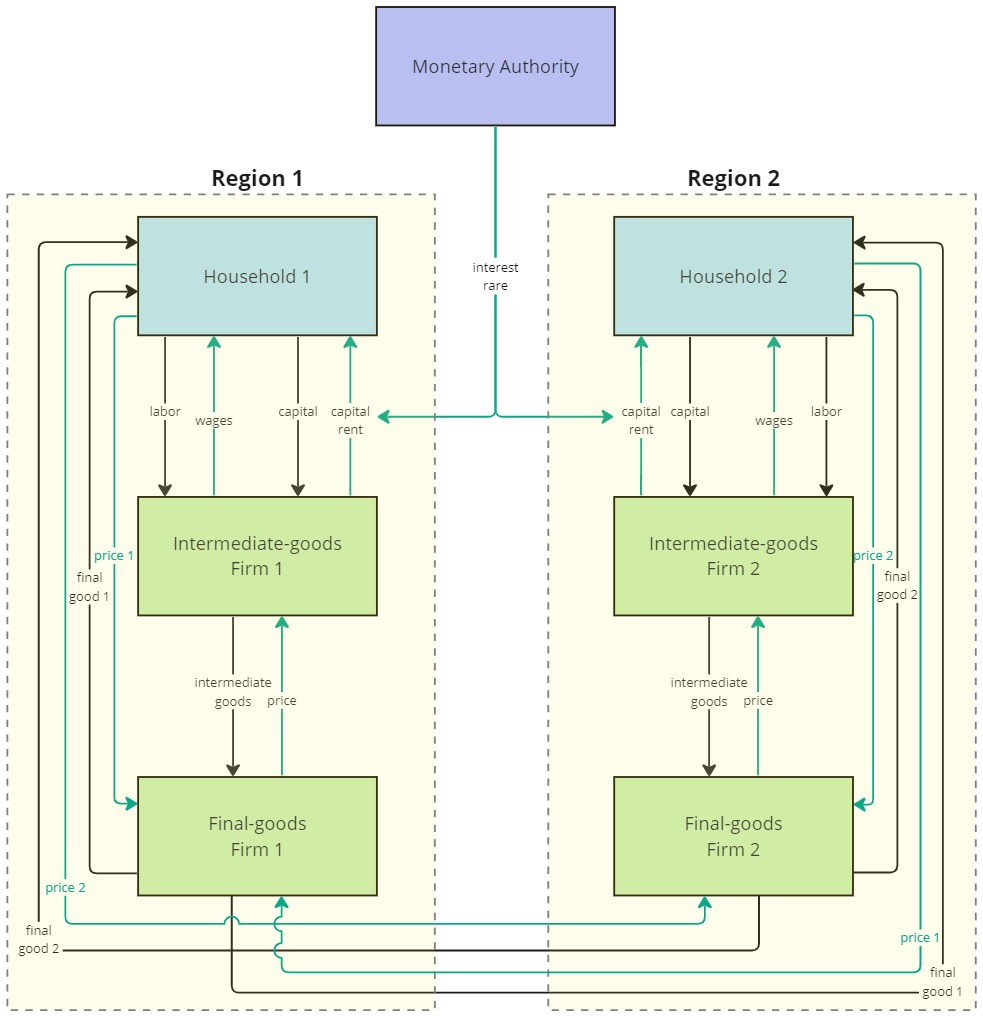
\includegraphics[width=\textwidth]{flowchart}
	\caption*{Source: created by the author.}
	\label{fig_v6:model-diagram}
\end{figure}	
	
% --------------------------------------------------
% REGIONAL MODEL
% --------------------------------------------------

% --------------------------------------------------
% HOUSEHOLD
% --------------------------------------------------

\newpage

\subsubsection{Household}

% The household problem can be split in two: first, they must minimize consumption costs, and then maximize utility subject to a budget constraint.

The household problem is divided into two steps: first, the household must minimize the consumption costs, and then maximize the utility, which is subject to a budget constraint.

\subsubsection*{Cost Minimization Problem}

Considering that the representative household must decide to consume goods from both regions, there must be a consumption bundle index $C_{\eta t}$ and a consumption price index $Q_{\eta t}$ that minimize the total consumption cost $Q_{\eta t} C_{\eta t}$, as demonstrated by \textcite[p.424]{walsh_monetary_2017}:
	\begin{align}
		\min_{C_{\eta 1 t}, C_{\eta 2 t}}: &\quad Q_{\eta t} C_{\eta t} = P_{1 t} C_{\eta 1t} + P_{2 t} C_{\eta 2t} \label{eq_v2:reg-consumption-cost}
		\\
		\st: &\quad C_{\eta t} = C_{\eta 1 t}^{\omega_{\eta 1}} C_{\eta 2 t}^{1-\omega_{\eta 1}} \label{eq_v2:reg-consumption-aggregation} \\
		&\quad C_{\eta t} > 0 \nonumber
	\end{align}

	where $P_{1t}$ and $P_{2t}$ are the prices of goods $1$ and $2$, respectively, $C_{\eta 1 t}$ and $C_{\eta 2 t}$ are the goods produced in region $1$ and $2$, respectively, and consumed in region $\eta$. In the consumption aggregation, ${\omega_{\eta 1}}$ and $({1 - \omega_{\eta 1}})$ are the weights of goods $C_{\eta 1 t}$ and $C_{\eta 2 t}$, respectively, in the consumption bundle $C_{\eta t}$.

\subsubsection*{Lagrangian}

% The minimization problem with restriction can be turned into one without restriction, applying the Lagrangian funcion:

The minimization problem with a constraint can be reformulated into one without a constraint by applying the Lagrangian function:
	\begin{align}
		\mathcal{L} &= P_{1 t} C_{\eta 1t} + P_{2 t} C_{\eta 2t} - Q_{\eta t} (C_{\eta 1 t}^{\omega_{\eta 1}} C_{\eta 2 t}^{1-\omega_{\eta 1}} - C_{\eta t}) \label{eq_v2:reg-consumption-lagrangian}
	\end{align}

\subsubsection*{First Order Conditions}

	The first order conditions are:
	\begin{align}
		C_{\eta 1 t}: &\quad P_{1 t} - Q_{\eta t} \omega_{\eta 1} C_{\eta 1 t}^{\omega_{\eta 1} - 1} C_{\eta 2 t}^{1-\omega_{\eta 1}} = 0 \implies \nonumber \\
		&\quad C_{\eta 1 t} = \frac{\omega_{\eta 1} Q_{\eta t} C_{\eta t}}{P_{1t}} \label{eq_v2:reg-C-eta1t}
		\\
		C_{\eta 2 t}: &\quad P_{2 t} - Q_{\eta t} (1 - \omega_{\eta 1}) C_{\eta 1 t}^{\omega_{\eta 1}} C_{\eta 2 t}^{-\omega_{\eta 1}} = 0 \implies \nonumber \\
		&\quad C_{\eta 2 t} = \frac{(1 - \omega_{\eta 1}) Q_{\eta t} C_{\eta t}}{P_{2t}} \label{eq_v2:reg-C-eta2t}
		\\
		Q_{\eta t}: &\quad C_{\eta t} = C_{\eta 1 t}^{\omega_{\eta 1}} C_{\eta 2 t}^{1-\omega_{\eta 1}} \tag{\ref{eq_v2:reg-consumption-aggregation}}
	\end{align}

\subsubsection*{Solutions}

	Divide \ref{eq_v2:reg-C-eta2t} by \ref{eq_v2:reg-C-eta1t}:
	\begin{align}
		\frac{C_{\eta 2 t}}{C_{\eta 1 t}} &= \frac{(1 - \omega_{\eta 1}) Q_{\eta t} C_{\eta t} / P_{2t}}{\omega_{\eta 1} Q_{\eta t} C_{\eta t} / P_{1t}} \implies \nonumber \\
		C_{\eta 2 t} &= C_{\eta 1 t} \frac{(1 - \omega_{\eta 1}) P_{1t}}{\omega_{\eta 1} P_{2t}} \label{eq_v2:reg-C-eta-12-t}
	\end{align}
	
	Substitute \ref{eq_v2:reg-C-eta-12-t} in \ref{eq_v2:reg-consumption-aggregation}:
	\begin{align}
		C_{\eta t} &= C_{\eta 1 t}^{\omega_{\eta 1}} \left[ C_{\eta 1 t} \frac{(1 - \omega_{\eta 1}) P_{1t}}{\omega_{\eta 1} P_{2t}} \right]^{1-\omega_{\eta 1}} \implies \nonumber \\
		C_{\eta 1 t} &= C_{\eta t} \left( \frac{P_{2t} \omega_{\eta 1}}{P_{1t} (1 - \omega_{\eta 1})} \right)^{1-\omega_{\eta 1}} \label{eq_v2:reg-C-eta-1-t}
	\end{align}

	Substitute \ref{eq_v2:reg-C-eta1t} and \ref{eq_v2:reg-C-eta2t} in \ref{eq_v2:reg-consumption-aggregation}:
	\begin{align}
		C_{\eta t} &= \left( \frac{\omega_{\eta 1} Q_{\eta t} C_{\eta t}}{P_{1t}} \right)^{\omega_{\eta 1}} \left( \frac{(1 - \omega_{\eta 1}) Q_{\eta t} C_{\eta t}}{P_{2t}} \right)^{1-\omega_{\eta 1}} \implies \nonumber \\
		Q_{\eta t} &= \left( \frac{P_{1 t}}{\omega_{\eta 1}} \right)^{\omega_{\eta 1}} \left( \frac{P_{2 t}}{1 -\omega_{\eta 1}} \right)^{1 -\omega_{\eta 1}} \label{eq_v2:reg-total-expense-level}
	\end{align}

\begin{comment}
	
		Divide \ref{eq_v2:reg-total-expense-level} of region 1 by region 2:
	\begin{align}
		\frac{Q_{1t}}{Q_{2t}} &= \frac{\left( \frac{P_{1 t}}{\omega_{11}} \right)^{\omega_{11}} \left( \frac{P_{2 t}}{1 -\omega_{11}} \right)^{1 -\omega_{11}}}{\left( \frac{P_{1 t}}{\omega_{21}} \right)^{\omega_{21}} \left( \frac{P_{2 t}}{1 -\omega_{21}} \right)^{1 -\omega_{21}}} \implies \nonumber \\
		\frac{Q_{1t}}{Q_{2t}} &= \frac{\omega_{21}^{\omega_{21}} (1 -\omega_{21})^{1 -\omega_{21}}}{\omega_{11}^{\omega_{11}} (1 - \omega_{11})^{1 - \omega_{11}}} \label{eq_v2:reg-total-expense-level-2}
	\end{align}
	
\end{comment}

	% Therefore, there is an consumption bundle $C_{\eta t}$ and a consumption price index $Q_{\eta t}$ that minimize the total consumption cost $Q_{\eta t} C_{\eta t}$ of household from region $\eta$. Notice that the cost problem of both regions are (must be) related, since the consumption level of one region influences the demand of goods from both regions. Now, this result will be used in the next problem the household faces.

	Therefore, there is a consumption bundle \(C_{\eta t}\) and a consumption price index \(Q_{\eta t}\) that minimize the total consumption cost \(Q_{\eta t} C_{\eta t}\) for the household in region \(\eta\). Notice that the cost problems of both regions are (must be) related, as the consumption level in one region influences the demand for goods in both regions. Now, this result will be used in the next problem that the household faces.

\subsubsection*{Utility Maximization Problem}

	Following the models presented by \textcite{costa_junior_understanding_2016} and \textcite{solis-garcia_ucb_2022}, the representative household next problem is to maximize an intertemporal utility function $U_{\eta}$ with respect to consumption $C_{\eta t}$ and labor $L_{\eta t}$, subject to a budget constraint, a capital accumulation rule and the non-negativity of real variables:
	\begin{align}
		\max_{C_{\eta t}, L_{\eta t}, K_{\eta,t+1}}: &\quad U_{\eta}(C_{\eta t},L_{\eta t}) = \E \sum_{t=0}^{\infty} \beta^t \left(\frac{C_{\eta t}^{1-\sigma}}{1-\sigma} - \phi \frac{L_{\eta t}^{1+\varphi}}{1+\varphi} \right) \label{eq_v2:reg-utility-function} 
		\\
		\st: &\quad Q_{\eta t} C_{\eta t} + P_{\eta t} I_{\eta t} = W_{\eta t} L_{\eta t} + R_{t} K_{\eta t} + \Pi_{\eta t} \label{eq_v2:reg-budget-constraint} \\
		&\quad K_{\eta,t+1} = (1 - \delta) K_{\eta t} + I_{\eta t} \label{eq_v2:reg-law-of-motion-of-capital} \\
		&\quad C_{\eta t}, L_{\eta t}, K_{\eta t} > 0 \nonumber
	\end{align}

	where $\E$ is the expectation operator, $\beta$ is the intertemporal discount factor, $\sigma$ is the relative risk aversion coefficient, $\phi$ is the relative labor weight in utility, $\varphi$ is the marginal disutility of labor supply. In the budget constraint,
	% $P_{1t}$ and $P_{2t}$ are the prices of goods $1$ and $2$, respectively, $C_{\eta 1 t}$ and $C_{\eta 2 t}$ are the goods produced in region $1$ and $2$, respectively, and consumed in region $\eta$,
	$I_{\eta t}$ is the investment,
	% $B_{\eta t}$ are the bonds, 
	$W_{\eta t}$ is the wage level,
	$K_{\eta t}$ is the capital, $R_{t}$ is the return on capital,
	% $R_t$ is the return on bonds (which is also the nominal interest rate of the economy) 
	and $\Pi_{\eta t}$ is the firm profit. In the capital accumulation rule, $\delta$ is the capital depreciation rate.
	% In the consumption aggregation, ${\omega_{\eta 1}}$ and ${1 - \omega_{\eta 1}}$ are the weights of goods $C_{\eta 1 t}$ and $C_{\eta 2 t}$, respectively, in the consumption bundle $C_{\eta t}$.

	Isolate $I_{\eta t}$ in \ref{eq_v2:reg-law-of-motion-of-capital} and substitute in \ref{eq_v2:reg-budget-constraint}:
	\begin{align}
		& I_{\eta t} = K_{\eta,t+1} - (1 - \delta) K_{\eta t} \label{eq_v2:reg-law-of-motion-of-capital-2} \\
		& Q_{\eta t} C_{\eta t} + P_{\eta t} (K_{\eta,t+1} - (1 - \delta) K_{\eta t}) = W_{\eta t} L_{\eta t} + R_{t} K_{\eta t} + \Pi_{\eta t} \label{eq_v2:reg-budget-constraint-2}
	\end{align}

\subsubsection*{Lagrangian}

	The maximization problem with restrictions can be transformed into one without restriction using the Lagrangian function $\mathcal{L}$ formed by \ref{eq_v2:reg-utility-function} and \ref{eq_v2:reg-budget-constraint-2}:
	\begin{align}
		\begin{split}
		& \mathcal{L} = \mathbb{E}_t \sum_{t=0}^{\infty} \beta^t \left\{ \left( \frac{C_{\eta t}^{1 -\sigma}}{1 -\sigma} - \phi \frac{L_{\eta t}^{1+\varphi}}{1+\varphi} \right) \right. - 
		\\ & \qquad - \left. \mu_{\eta t} \Big[ Q_{\eta t} C_{\eta t} + P_{\eta t} (K_{\eta,t+1} - (1 - \delta) K_{\eta t}) - (W_{\eta t} L_{\eta t} + R_{t} K_{\eta t} + \Pi_{\eta t}) \Big] \right\} \label{eq_v2:reg-household-lagrangian}
		\end{split}
	\end{align}

\subsubsection*{First Order Conditions}

The first order conditions are:
\begin{align}
	C_{\eta t}: &\quad \beta^t \left\{ \frac{(1 -\sigma) C_{\eta t}^{-\sigma}}{1-\sigma} - \mu_{\eta t} \left[ Q_{\eta t} \right] \right\} = 0 \implies \nonumber \\
	&\quad \mu_{\eta t} = \frac{C_{\eta t}^{-\sigma}}{Q_{\eta t}} \label{eq_v2:reg-FOC-C-eta-t}
	\\
	L_{\eta t}: &\quad \beta^t \left\{ -\phi \frac{(1+\varphi) L_{\eta t}^{1 + \varphi}}{1 + \varphi} - \mu_{\eta t} \left[ -W_{\eta t} \right] \right\} = 0 \implies \nonumber \\
	&\quad \mu_{\eta t} = \frac{\phi L_{\eta t}^{\varphi}}{W_{\eta t}} \label{eq_v2:reg-FOC-Lt}
	\\
	K_{\eta,t+1}: &\quad \beta^t \{-\mu_{\eta t} [P_{\eta t}] \} + \mathbb{E}_{t} \beta^{t+1} \{ -\mu_{\eta,t+1} [-(P_{\eta,t+1} (1 - \delta) + R_{t+1})] \} = 0 \implies \nonumber \\
	&\quad \mu_{\eta t} P_{\eta t} = \beta \mathbb{E}_{t} \{ \mu_{\eta,t+1} [P_{\eta,t+1} (1 - \delta) + R_{t+1}] \} \label{eq_v2:reg-FOC-Kt}
	% B_{\eta t}: &\quad \beta^t \{-\mu_{\eta t}\} + \E \beta^{t+1} \{ -\mu_{\eta, t+1} [-(1 + R_{t})] \} = 0 \implies \nonumber
	% \\ &\quad \mu_{\eta t} = \beta (1 + R_{t}) \E{ \mu_{\eta, t+1}} \label{eq_v2:reg-FOC-Bt}
	\\
	\mu_{\eta t}: &\quad Q_{\eta t} C_{\eta t} + P_{\eta t} (K_{\eta,t+1} - (1 - \delta) K_{\eta t}) = W_{\eta t} L_{\eta t} + R_{t} K_{\eta t} + \Pi_{\eta t} \tag{\ref{eq_v2:reg-budget-constraint-2}}
\end{align}

\subsubsection*{Solutions}

Match \ref{eq_v2:reg-FOC-C-eta-t} and \ref{eq_v2:reg-FOC-Lt}:
\begin{align}
	\mu_{\eta t} = \frac{ C_{\eta t}^{-\sigma}}{Q_{\eta t}} &= \frac{\phi L_{\eta t}^{\varphi}}{W_{\eta t}} \implies \nonumber \\
	\frac{\phi L_{\eta t}^{\varphi}}{C_{\eta t}^{-\sigma}} &= \frac{W_{\eta t}}{Q_{\eta t}} \label{eq_v2:reg-labor-supply}
\end{align}

Equation \ref{eq_v2:reg-labor-supply} is the Household Labor Supply and shows that the marginal rate of substitution (MRS) of labor for consumption is equal to the real wage, which is the relative price between labor and goods.

Substitute $\mu_{\eta t}$ and $\mu_{\eta, t+1}$ from equation \ref{eq_v2:reg-FOC-C-eta-t} in \ref{eq_v2:reg-FOC-Kt}:
\begin{alignat}{2}
	\frac{C_{\eta t}^{-\sigma}}{Q_{\eta t}} P_{\eta t} &= \beta \mathbb{E}_{t} \left\{ \frac{C_{\eta t}^{-\sigma}}{Q_{\eta t}} [P_{\eta,t+1} (1 - \delta) + R_{t+1}] \right\} \implies \nonumber \\
	\frac{\mathbb{E}_{t} \{ Q_{\eta,t+1} C_{\eta,t+1}^{\sigma} \} }{ Q_{\eta t} C_{\eta t}^{\sigma} } &= \beta \frac{ \mathbb{E}_{t} \{ P_{\eta,t+1} (1 - \delta) + R_{t+1} \} }{P_{\eta t}} \label{eq_v2:reg-capital-euler-equation}
\end{alignat}

%%%%%%%%%%%%%%%%%%%%%%%%%%%%%%%%%%%%%%%%%%%%%%%%%%

Equation \ref{eq_v2:reg-capital-euler-equation} is the Euler equation for the return on capital.

\begin{comment}

	Divide \ref{eq_v2:reg-capital-euler-equation} of region one by region two:
\begin{alignat}{2}
	\frac{\mathbb{E}_{t} \left\{Q_{1, t+1} C_{1, t+1}^{\sigma} \right\}}{\mathbb{E}_{t} \left\{Q_{2, t+1} C_{2, t+1}^{\sigma} \right\}} &= \frac{\beta (1 + R_{t}) Q_{1t} C_{1t}^{\sigma}}{\beta (1 + R_{t}) Q_{2t} C_{2t}^{\sigma}} \implies \nonumber \\
	\frac{\mathbb{E}_{t} \left\{ Q_{1, t+1} C_{1, t+1}^{\sigma} \right\}}{Q_{1t} C_{1t}^{\sigma}} &= \frac{\mathbb{E}_{t} \left\{ Q_{2, t+1} C_{2, t+1}^{\sigma} \right\}}{Q_{2t} C_{2t}^{\sigma}} \label{eq_v2:reg-bonds-euler-equation-2}
\end{alignat}
	
\end{comment}

%%%%%%%%%%%%%%%%%%%%%%%%%%%%%%%%%%%%%%%%%%%%%%%%%%

\begin{comment}

	Define the regional consumer inflation gross rate:
	\begin{align}
		\pi_{\eta t} &= \frac{Q_{\eta t}}{Q_{\eta, t-1}} \label{eq_v2:consumer-inflation}
	\end{align}

	The relation between the nominal $R_{t}$ and the real $r_{t}$ interest rates is the gross inflation rate $\pi_{t}$, given by the Fisher equation. % As the interest rate is common to both regions the regional inflations must be equal:
	\begin{align}
		\pi_{t} = \frac{(1 + R_{t})}{(1 + r_{t})}  \label{eq_v2:fisher-equation}
	\end{align}
	
\end{comment}

%%%%%%%%%%%%%%%%%%%%%%%%%%%%%%%%%%%%%%%%%%%%%%%%%%

% --------------------------------------------------
% FIRMS
% --------------------------------------------------

\subsubsection*{Firms}

Consider two types of firms: 
\begin{enumerate*}[label=(\arabic*)]
	\item a continuum of intermediate-goods firms, which operate in monopolistic competition and each produce one variety with imperfect substitution level between each other and
	\item the final-goods firm, which aggregates all these varieties into a final bundle and operates in perfect competition.
\end{enumerate*}

% --------------------------------------------------
% final-goods FIRM
% --------------------------------------------------

\subsubsection{Final-Goods Firm}

\subsubsection*{Profit Maximization Problem}

The role of the final-goods firm is to aggregate all the varieties $Y_{\eta jt}$ produced by the intermediate-goods firms in each region $\eta \in \{1,2\}$, so that the representative consumer can buy only one good $Y_{\eta t}$, the bundle good, from each region.

% The role of the final-goods firm is to aggregate all the varieties produced by the intermediate-goods firms, so that the representative consumer can buy only one good $Y_{\eta t}$, the bundle good.

% There are two regions and each region has a representative final-goods firm. The first region has a continuum of intermediate-goods firms indexes by $j \in [0,j_m]$ and the second region has firms indexed by $j \in \mathopen( j_m,1 \mathclose]$.\footnote{note that if $j_m > \sfrac{1}{2}$, then region $m$ is more industrious than region $m+1$.}

The final-goods firm problem is to maximize its profit, considering that its output is the bundle $Y_{\eta t}$ formed by a continuum $j \in [0,1]$ of intermediate-goods $Y_{\eta jt}$, with elasticity of substitution between intermediate-goods $\psi$:
\begin{align}
	\max_{Y_{\eta jt}}: &\quad P_{\eta t} Y_{\eta t} - \int_{0}^{1} P_{\eta jt} Y_{\eta jt} \dif j \label{eq_v2:reg-final-goods-firm-max-problem} \\
	\st: & \quad Y_{\eta t} = \left( \int_{0}^{1} Y_{\eta jt}^{\frac{\psi-1}{\psi}} \dif j \right)^{\frac{\psi}{\psi-1}} \label{eq_v2:reg-final-goods-firm-bundle-rule}
\end{align}

Substitute \ref{eq_v2:reg-final-goods-firm-bundle-rule} in \ref{eq_v2:reg-final-goods-firm-max-problem}:
\begin{align}
	\label{eq_v2:reg-final-goods-firm-max-problem-2}
	\max_{Y_{\eta jt}}: & \quad \Pi_{\eta t} = P_{\eta t} \left( \int_{0}^{1} Y_{\eta jt}^{\frac{\psi-1}{\psi}} \dif j \right)^{\frac{\psi}{\psi-1}} - \int_{0}^{1} P_{\eta jt} Y_{\eta jt} \dif j
\end{align}

\subsubsection*{First Order Condition and Solutions}

The first order condition is:
\begin{align}
	Y_{\eta jt}:\quad & P_{\eta t} \left( \frac{\psi}{\psi-1} \right) \left( \int_{0}^{1} Y_{\eta jt}^{\frac{\psi-1}{\psi}} \dif j \right)^{\frac{\psi}{\psi-1}-1} \left( \frac{\psi-1}{\psi} \right) Y_{\eta jt}^{\frac{\psi-1}{\psi}-1} - P_{\eta jt} = 0 \implies \nonumber \\
	\label{eq_v2:reg-final-goods-firm-FOC}
	& Y_{\eta jt} = Y_{t} \left( \frac{P_{\eta t}}{P_{\eta jt}} \right)^{\psi}
\end{align}

Equation \ref{eq_v2:reg-final-goods-firm-FOC} shows that the demand for variety $j$ depends on its relative price. 

Substitute \ref{eq_v2:reg-final-goods-firm-FOC} in \ref{eq_v2:reg-final-goods-firm-bundle-rule}:
\begin{alignat}{2}
	Y_{\eta t} & = \left( \int_{0}^{1} Y_{\eta jt}^{\frac{\psi-1}{\psi}} \dif j \right)^{\frac{\psi}{\psi-1}} &\implies \nonumber \\
	Y_{\eta t} & = \left( \int_{0}^{1} \left[ Y_{\eta t} \left( \frac{P_{\eta t}}{P_{\eta jt}} \right)^{\psi} \right]^{\frac{\psi-1}{\psi}} \dif j \right)^{\frac{\psi}{\psi-1}} \quad &\implies \nonumber \\
	P_{\eta t} & = \left[ \int_{0}^{1} P_{\eta jt}^{1-\psi} \dif j \right]^{\frac{1}{1-\psi}} \label{eq_v2:reg-final-goods-firm-markup}
\end{alignat}

Equation \ref{eq_v2:reg-final-goods-firm-markup} is the final-goods firm's markup.

% --------------------------------------------------
% intermediate-goods FIRM
% --------------------------------------------------

\subsubsection{Intermediate-Goods Firms}

\subsubsection*{Cost Minimization Problem}

The intermediate-goods firms, denoted by $j \in [0,1]$, produce varieties of a representative good with a certain level of substitutability. Each of these firms has to choose labor $L_{\eta jt}$ to minimize production costs, subject to a technology rule.
\begin{align}
	\label{eq_v2:reg-int-good-firm-total-cost}
	\min_{K_{\eta jt}, L_{\eta jt}}: \quad & R_{Kt} K_{\eta jt} + W_t L_{\eta jt} \\
	\label{eq_v2:reg-int-good-firm-prod-function}
	\st: \quad & Y_{\eta jt} = Z_{A\eta t} K_{\eta jt}^{\alpha_{\eta}} L_{\eta jt}^{1-{\alpha_{\eta}}}
\end{align}

\begin{comment}
	
	\begin{tcolorbox}[colback=red!5!white,colframe=red!75!black]
		“We set this parameter so that profits are zero in steady state” [Adolfson et al., 2014, p. 36] 
	\end{tcolorbox}	

\end{comment}

where $Y_{\eta jt}$ is the output obtained by the production technology level $Z_{A\eta t}$ that transforms capital $K_{\eta jt}$ and labor $L_{\eta jt}$ in proportions ${\alpha_{\eta}}$ and $(1-{\alpha_{\eta}})$, respectively, into intermediate goods.\footnote{the production technology level $Z_{A\eta t}$ will be submitted to a productivity shock, detailed in section \ref{sec_v6:reg-productivity-shock}.}

\subsubsection*{Lagrangian}

Transform the minimization problem with restriction into one without restriction applying the Lagrangian function $\mathcal{L}$:
\begin{align}
	\label{eq_v2:reg-int-good-firm-lagrangian}
	\mathcal{L} = (R_{Kt} K_{\eta jt} + W_t L_{\eta jt}) - \Lambda_{\eta jt} (Z_{A\eta t} K_{\eta jt}^{\alpha_{\eta}} L_{\eta jt}^{1-{\alpha_{\eta}}} - Y_{\eta jt})
\end{align}

where the Lagrangian multiplier $\Lambda_{\eta jt}$ is the marginal cost.\footnote{see Lemma \ref{lemma:marginal-cost}}

\subsubsection*{First Order Condition}

The first-order conditions are:
\begin{alignat}{2}
	K_{\eta jt}: \quad & R_{Kt} - \Lambda_{\eta jt} Z_{A\eta t} {\alpha_{\eta}} K_{\eta jt}^{{\alpha_{\eta}}-1} L_{\eta jt}^{1-{\alpha_{\eta}}} = 0 &&\implies \nonumber \\
	& K_{\eta jt} = {\alpha_{\eta}} Y_{\eta jt} \frac{\Lambda_{\eta jt}}{R_{Kt}} \label{eq_v2:reg-int-good-firm-FOC-Kt} \\
	L_{\eta jt}: \quad & W_t - \Lambda_{\eta jt} Z_{A\eta t} K_{\eta jt}^{\alpha_{\eta}} (1-{\alpha_{\eta}}) L_{\eta jt}^{-{\alpha_{\eta}}} = 0 \quad &&\implies \nonumber \\ 
	& L_{\eta jt} = (1-{\alpha_{\eta}}) Y_{\eta jt} \frac{\Lambda_{\eta jt}}{W_t} \label{eq_v2:reg-int-good-firm-FOC-Lt-0} \\
	\Lambda_{\eta jt}: \quad & Y_{\eta jt} = Z_{A\eta t} K_{\eta jt}^{\alpha_{\eta}} L_{\eta jt}^{1-{\alpha_{\eta}}} \tag{\ref{eq_v2:reg-int-good-firm-prod-function}}
\end{alignat}

\subsubsection*{Solutions}

Divide equation \ref{eq_v2:reg-int-good-firm-FOC-Kt} by \ref{eq_v2:reg-int-good-firm-FOC-Lt-0}:
\begin{align}
	\frac{K_{\eta jt}}{L_{\eta jt}} = \frac{{\alpha_{\eta}} Y_{\eta jt} \Lambda_{\eta jt} /R_{Kt}}{(1-\alpha_{\eta}) Y_{\eta jt} \Lambda_{\eta jt} /W_{\eta t}} \implies
	\frac{K_{\eta jt}}{L_{\eta jt}} = \left( \frac{{\alpha_{\eta}}}{1-\alpha_{\eta}} \right) \frac{W_{\eta t}}{R_{Kt}} \label{eq_v2:reg-int-good-firm-TMRS}
\end{align}

Equation \ref{eq_v2:reg-int-good-firm-TMRS} demonstrates the relationship between the technical marginal rate of substitution (TMRS) and the economic marginal rate of substitution (EMRS). 

Substitute $L_{\eta jt}$ from equation \ref{eq_v2:reg-int-good-firm-TMRS} in \ref{eq_v2:reg-int-good-firm-prod-function}:
\begin{alignat}{2}
	Y_{\eta jt} & = Z_{A\eta t} K_{\eta jt}^{\alpha_{\eta}} L_{\eta jt}^{1-\alpha_{\eta}} &\implies \nonumber \\
	Y_{\eta jt} & = Z_{A\eta t} K_{\eta jt}^{\alpha_{\eta}} \left[ \left( \frac{1-\alpha_{\eta}}{{\alpha_{\eta}}} \right) \frac{R_{Kt} K_{\eta jt}}{W_{\eta t}} \right]^{1-\alpha_{\eta}} &\implies \nonumber \\
	K_{\eta jt} & = \frac{Y_{\eta jt}}{Z_{A\eta t}} \left[ \left( \frac{{\alpha_{\eta}}}{1-\alpha_{\eta}} \right) \frac{W_{\eta t}}{R_{Kt}}\right]^{1-\alpha_{\eta}} \label{eq_v2:reg-int-good-firm-Kt-demand}
\end{alignat}

Equation \ref{eq_v2:reg-int-good-firm-Kt-demand} is the intermediate-goods firm demand for capital. 

Substitute \ref{eq_v2:reg-int-good-firm-Kt-demand} in \ref{eq_v2:reg-int-good-firm-TMRS}:
\begin{alignat}{2}
	L_{\eta jt} & = \left( \frac{1-\alpha_{\eta}}{{\alpha_{\eta}}} \right) \frac{R_{Kt} K_{\eta jt}}{W_{\eta t}} &\implies \nonumber \\
	L_{\eta jt} & = \left( \frac{1-\alpha_{\eta}}{{\alpha_{\eta}}} \right) \frac{R_{Kt}}{W_{\eta t}} \frac{Y_{\eta jt}}{Z_{A\eta t}} \left[ \left( \frac{{\alpha_{\eta}}}{1-\alpha_{\eta}} \right) \frac{W_{\eta t}}{R_{Kt}}\right]^{1-\alpha_{\eta}} &\implies \nonumber \\
	L_{\eta jt} & = \frac{Y_{\eta jt}}{Z_{A\eta t}} \left[ \left( \frac{{\alpha_{\eta}}}{1-\alpha_{\eta}} \right) \frac{W_{\eta t}}{R_{Kt}}\right]^{-{\alpha_{\eta}}} \label{eq_v2:reg-int-good-firm-Lt-demand}
\end{alignat}

Equation \ref{eq_v2:reg-int-good-firm-Lt-demand} is the intermediate-goods firm demand for labor.

\subsubsection*{Total and Marginal Costs}

Calculate the total cost $TC$ using \ref{eq_v2:reg-int-good-firm-Kt-demand} and \ref{eq_v2:reg-int-good-firm-Lt-demand}:
\begin{alignat}{2}
	TC_{\eta jt} & = W_{\eta t} L_{\eta jt} + R_{Kt} K_{\eta jt} &\implies \nonumber \\
	TC_{\eta jt} & = W_{\eta t} \frac{Y_{\eta jt}}{Z_{A\eta t}} \left[ \left( \frac{{\alpha_{\eta}}}{1-\alpha_{\eta}} \right) \frac{W_{\eta t}}{R_{Kt}} \right]^{-{\alpha_{\eta}}} + R_{Kt} \frac{Y_{\eta jt}}{Z_{A\eta t}} \left[ \left( \frac{{\alpha_{\eta}}}{1-\alpha_{\eta}} \right) \frac{W_{\eta t}}{R_{Kt}} \right]^{1-\alpha_{\eta}} &\implies \nonumber \\
	TC_{\eta jt} & = \frac{Y_{\eta jt}}{Z_{A\eta t}} \left( \frac{R_{Kt}}{{\alpha_{\eta}}} \right)^{{\alpha_{\eta}}} \left( \frac{W_{\eta t}}{1-\alpha_{\eta}} \right)^{1-\alpha_{\eta}} \label{eq_v2:reg-int-good-firm-TC}
\end{alignat}

%%%%%

Calculate the marginal cost $\Lambda$ using \ref{eq_v2:reg-int-good-firm-TC}: 
\begin{align}
	\Lambda_{\eta jt} & = \frac{\partial TC_{\eta jt}}{\partial Y_{\eta jt}} \implies 
	\Lambda_{\eta jt} = \frac{1}{Z_{A\eta t}} \left( \frac{R_{Kt}}{{\alpha_{\eta}}} \right)^{{\alpha_{\eta}}} \left( \frac{W_{\eta t}}{1-\alpha_{\eta}} \right)^{1-\alpha_{\eta}} \label{eq_v2:reg-int-good-firm-MC}
\end{align}

The marginal cost depends on the technological level $Z_{A\eta t}$, the nominal interest rate $R_{Kt}$ and the nominal wage level $W_{\eta t}$, which are the same for all intermediate-goods firms, and because of that, the index $j$ may be dropped:
\begin{align}
	\Lambda_{\eta t} = \frac{1}{Z_{A\eta t}} \left( \frac{R_{Kt}}{{\alpha_{\eta}}} \right)^{{\alpha_{\eta}}} \left( \frac{W_{\eta t}}{1-\alpha_{\eta}} \right)^{1-\alpha_{\eta}} \label{eq_v2:reg-int-good-firm-MC-2}
\end{align}

notice that:
\begin{align}
	\Lambda_{\eta t} = \frac{TC_{\eta jt}}{Y_{\eta jt}} \implies 
	TC_{\eta jt} = \Lambda_{\eta t} Y_{\eta jt} \label{eq_v2:reg-int-good-firm-TC-MC}
\end{align}

\begin{comment}
	
As salaries and technology are the same for all firms in region $\eta$, the $j$ index can be dropped from the marginal cost $\Lambda$:
\begin{alignat}{2}
	\Lambda_{\eta t} = \frac{W_{\eta t}}{Z_{A\eta t}} \label{eq_v2:reg-int-good-firm-prod-function}
\end{alignat}

Notice that:
\begin{align}
	TC_{\eta jt} &= W_{\eta t} L_{\eta jt} = \Lambda_{\eta t} Y_{\eta jt} 
	%\label{eq_v2:reg-int-good-firm-TC-MC} \\
	MC_{\eta jt} &= \frac{\partial TC_{\eta jt}}{\partial Y_{\eta jt}} = \Lambda_{\eta t} \nonumber
\end{align}

\end{comment}

% --------------------------------------------------
% CALVO RULE
% --------------------------------------------------

\subsubsection*{Optimal Price Problem}

Consider an economy with price stickiness, following the Calvo Rule \cite{calvo_staggered_1983}: each firm has a probability $(0 < \theta < 1)$ of keeping its price in the next period ($P_{\eta j,t+1} = P_{\eta jt}$), and a probability $(1 - \theta)$ of setting a new optimal price $P_{\eta jt}^{\ast}$ that maximizes its profits. Therefore, each firm must take this uncertainty into account when deciding the optimal price: the intertemporal profit flow, given the nominal interest rate $R_{t}$ of each period, is calculated considering the probability $\theta$ of keeping the previous price:
\begin{align}
	\label{eq_v2:reg-int-good-firm-optimal-price-problem}
	\max_{P_{\eta jt}}: & \quad \E \sum_{s=0}^{\infty} \left\{ \frac{ \theta^s \left[ P_{\eta jt} Y_{\eta j,t+s} - TC_{\eta j,t+s} \right]}{\prod_{k=0}^{s-1}(1+R_{t+k})} \right\} \\
	\tag{\ref{eq_v2:reg-final-goods-firm-FOC}}
	\st: & \quad Y_{\eta jt} = Y_{\eta t} \left( \frac{P_{\eta t}}{P_{\eta jt}} \right)^{\psi}
\end{align}

where $s$ is the period in time when the decision must be made; $t$ is the last period in time when the price was updated and $k$ is the period in the future when the interest rate applies.

%%%%%

Substitute \ref{eq_v2:reg-int-good-firm-TC-MC} in \ref{eq_v2:reg-int-good-firm-optimal-price-problem}:
\begin{align}
	\label{eq_v2:reg-int-good-firm-optimal-price-problem-2}
	\max_{P_{\eta jt}}: & \quad \E \sum_{s=0}^{\infty} \left\{ \frac{\theta^s \big[ P_{\eta jt} Y_{\eta j,t+s} - \Lambda_{\eta, t+s} Y_{\eta j,t+s} \big]}{\prod_{k=0}^{s-1}(1+R_{t+k})} \right\}
\end{align}

Substitute \ref{eq_v2:reg-final-goods-firm-FOC} in \ref{eq_v2:reg-int-good-firm-optimal-price-problem-2} and rearrange the variables:
\begin{align}
	\max_{P_{\eta jt}}: & \quad \E \sum_{s=0}^{\infty} \left\{ \frac{\theta^s \left[ P_{\eta jt} Y_{\eta t+s} \left( \frac{P_{\eta, t+s}}{P_{\eta jt}} \right)^{\psi} - \Lambda_{\eta, t+s} Y_{\eta t+s} \left( \frac{P_{\eta, t+s}}{P_{\eta jt}} \right)^{\psi} \right]}{\prod_{k=0}^{s-1}(1+R_{t+k})} \right\} \implies \nonumber 
	\\
	\max_{P_{\eta jt}}: & \quad \E \sum_{s=0}^{\infty} \left\{ \frac{\theta^s \left[ P_{\eta jt}^{1-\psi} P_{\eta, t+s}^{\psi} Y_{\eta t+s} - P_{\eta jt}^{-\psi} P_{\eta, t+s}^{\psi} Y_{\eta t+s} \Lambda_{\eta, t+s} \right]}{\prod_{k=0}^{s-1}(1+R_{t+k})} \right\} \nonumber
\end{align}

%%%%%

\subsubsection*{First Order Condition}

The first order condition with respect to $P_{\eta jt}$ is:
\begin{align}
	& \quad \E \sum_{s=0}^{\infty} \left\{ \frac{\theta^s \left[ (1-\psi) P_{\eta jt}^{-\psi} P_{\eta, t+s}^{\psi} Y_{\eta t+s} - (-\psi) P_{\eta jt}^{-\psi-1} P_{\eta, t+s}^{\psi} Y_{\eta t+s} \Lambda_{\eta, t+s} \right]}{\prod_{k=0}^{s-1}(1+R_{t+k})} \right\} = 0 \nonumber
\end{align}

%%%%%

Separate the summations and rearrange the variables:
\begin{align}
	\begin{split}
		\E \sum_{s=0}^{\infty} &\left\{ \frac{\theta^s (\psi-1) \left( \frac{P_{\eta, t+s}} {P_{\eta jt}} \right)^{\psi} Y_{\eta t+s}} {\prod_{k=0}^{s-1} (1+R_{t+k})} \right\} = \\
		&= \E \sum_{s=0}^{\infty} \left\{ \frac{\theta^s \psi P_{\eta jt}^{-1} \left( \frac{P_{\eta, t+s}} {P_{\eta jt}} \right)^{\psi} Y_{\eta t+s} \Lambda_{\eta, t+s}}{\prod_{k=0}^{s-1}(1+R_{t+k})} \right\} \label{eq_v2:reg-int-good-firm-optimal-price-FOC}
	\end{split}
\end{align}

%%%%%

Substitute \ref{eq_v2:reg-final-goods-firm-FOC} in \ref{eq_v2:reg-int-good-firm-optimal-price-FOC}:
\begin{alignat}{2}
	\E \sum_{s=0}^{\infty} \Bigg\{ \frac{\theta^s (\psi-1) Y_{\eta j,t+s}}{\prod_{k=0}^{s-1}(1+R_{t+k})} \Bigg\} &= \E \sum_{s=0}^{\infty} \Bigg\{ \frac{\theta^s \psi P_{\eta jt}^{-1} Y_{\eta j,t+s} \Lambda_{\eta, t+s}}{\prod_{k=0}^{s-1}(1+R_{t+k})}  \Bigg\} &\implies \nonumber \\
	(\psi-1) \E \sum_{s=0}^{\infty} \Bigg\{ \frac{\theta^s Y_{\eta j,t+s}}{\prod_{k=0}^{s-1}(1+R_{t+k})} \Bigg\} &= \psi P_{\eta jt}^{-1} \E \sum_{s=0}^{\infty} \Bigg\{ \frac{\theta^s Y_{\eta j,t+s} \Lambda_{\eta, t+s}}{\prod_{k=0}^{s-1}(1+R_{t+k})}  \Bigg\} &\implies \nonumber \\
	P_{\eta jt} \E \sum_{s=0}^{\infty} \Bigg\{ \frac{\theta^s Y_{\eta j,t+s}}{\prod_{k=0}^{s-1}(1+R_{t+k})} \Bigg\} &= \frac{\psi}{\psi-1} \E \sum_{s=0}^{\infty} \Bigg\{ \frac{\theta^s Y_{\eta j,t+s} \Lambda_{\eta, t+s}}{\prod_{k=0}^{s-1}(1+R_{t+k})}  \Bigg\} &\implies \nonumber
\end{alignat}

\vspace*{-1cm}

\begin{align}
	\label{eq_v2:reg-int-good-firm-optimal-price-FOC-2}
	P_{\eta jt}^{\ast} &= 
	\frac{\psi}{\psi-1} \cdot
	\frac{
		\E \sum_{s=0}^{\infty} \left\{ 
		\theta^s Y_{\eta j,t+s} \Lambda_{\eta, t+s} / \prod_{k=0}^{s-1}(1+R_{t+k}) \right\}} {\E \sum_{s=0}^{\infty} \left\{
		\theta^s Y_{\eta j,t+s} / \prod_{k=0}^{s-1}(1+R_{t+k}) \right\}}
\end{align}

%%%%%

Equation \ref{eq_v2:reg-int-good-firm-optimal-price-FOC-2} represents the optimal price that firm $j$ will choose. Since all firms that are able to choose will opt for the highest possible price, they will all select the same price. As a result, the index $j$ can be omitted:
\begin{align}
	\label{eq_v2:reg-int-good-firm-optimal-price-FOC-3}
	P_{\eta t}^{\ast} &= 
	\frac{\psi}{\psi-1} \cdot
	\frac{
		\E \sum_{s=0}^{\infty} \left\{ 
		\theta^s Y_{\eta j,t+s} \Lambda_{\eta, t+s} / \prod_{k=0}^{s-1}(1+R_{t+k}) \right\}} {\E \sum_{s=0}^{\infty} \left\{
		\theta^s Y_{\eta j,t+s} / \prod_{k=0}^{s-1}(1+R_{t+k}) \right\}}
\end{align}

% --------------------------------------------------
% final-goods FIRM, PART II
% --------------------------------------------------

\subsubsection*{Final-Goods Firm, part II}

The process of fixing prices is random: in each period, $\theta$ firms will maintain the price from the previous period, while $(1-\theta)$ firms will choose a new optimal price. The price level for each period will be a composition of these two prices. Use this information in \ref{eq_v2:reg-final-goods-firm-markup} to determine the aggregate price level:
\begin{align}
	P_{\eta t} & = \left[ \int_{0}^{\theta} P_{\eta, t-1}^{1-\psi} \dif j + \int_{\theta}^{1} P_{\eta t}^{\ast 1-\psi} \dif j \right]^{\frac{1}{1-\psi}}  \implies \nonumber \\
	P_{\eta t} & = \left[ \theta P_{\eta, t-1}^{1-\psi} + (1-\theta) P_{\eta t}^{\ast 1-\psi} \right]^\frac{1}{1-\psi} \label{eq_v2:reg-general-price-level}
\end{align}

Equation \ref{eq_v2:reg-general-price-level} is the aggregate price level.

% --------------------------------------------------
% REGIONAL INFLATION
% --------------------------------------------------

\subsubsection*{Regional Inflation}

In each region, the price level $P_{\eta t}$ generates a regional inflation rate:
\begin{align}
	\pi_{\eta t} = \frac{P_{\eta t}}{P_{\eta, t-1}} \label{eq_v2:reg-regional-inflation}
\end{align}

% --------------------------------------------------
% MONETARY AUTHORITY
% --------------------------------------------------

\subsubsection{Monetary Authority}

The objective of the monetary authority is to conduct the economy to price stability and economic growth, using a Taylor rule \cite{taylor_discretion_1993} to determine the nominal interest rate:
\begin{align}
	\label{eq_v2:reg-monetary-policy}
	\frac{R_{t}}{R} =
	\left( \frac{R_{t-1}}{R} \right)^{\gamma_{R}}  \left[
	\left( \frac{\pi_t}{\pi} \right)^{\gamma_{\pi}}
	\left( \frac{Y_{t}}{Y} \right)^{\gamma_{Y}} \right]^{1-\gamma_{R}} Z_{Mt}
\end{align}

where $R, \pi, Y$ are the nominal interest rate, gross inflation rate and the production level in steady state, respectively; $\gamma_{R}$ is the smoothing parameter for the interest rate $R_{Kt}$, $\gamma_{\pi}$ and $\gamma_{Y}$ are the interest-rate sensitivities in relation to inflation and product, respectively, $Z_{Mt}$ is the monetary shock and $\pi_t$ is the gross inflation rate, defined by:\footnote{for the monetary shock definition, see section \ref{sec_v6:reg-monetary-shock}.}
\begin{align}
	\pi_{t} &= \pi_{1t}^{\theta_{\pi}} \pi_{2t}^{1 - \theta_{\pi}}
	\label{eq_v2:reg-gross-inflation-rate} \\ 
	&\quad \text{where: } \theta_{\pi} = \frac{P_{1t} Y_{1t}}{P_{1t} Y_{1t} + P_{2t} Y_{2t}} \label{eq_v2:reg-theta-pi}
\end{align}

\begin{comment}

where $P_t$ is the national price level, defined by:
\begin{align}
	P_{t} Y_{t} &= P_{1t} Y_{1t} + P_{2t} Y_{2t} \iff P_{t} = \frac{P_{1t} Y_{1t} + P_{2t} Y_{2t}}{Y_{t}} \label{eq_v2:reg-national-price-level}
\end{align}
	
	\begin{align}
		P_{t} Y_{t} &= P_{1t} Y_{1t} + P_{2t} Y_{2t} \implies \nonumber \\
		P_{t} &= \frac{Y_{1t}}{Y_{t}} P_{1t} + \frac{Y_{2t}}{Y_{t}} P_{2t} \implies \nonumber \\
		P_{t} &= \theta_{P1} P_{1t} + (1 -\theta_{P1}) P_{2t} %\label{eq_v2:reg-national-price-level}
	\end{align}
	
	where $\theta_{P1}$ and $(1-\theta_{P1})$ are the price level weights of regions 1 and 2 in the national price level composition, respectively:
	\begin{align}
		\left\langle \begin{matrix} \theta_{P1} & (1-\theta_{P1}) \end{matrix} \right\rangle \coloneq \left\langle \begin{matrix} \frac{Y_{1t}}{Yt} & \frac{Y_{2t}}{Yt} \end{matrix} \right\rangle \label{eq_v2:reg-ss-P1-P2-weight-in-P}
	\end{align}
\end{comment}

% --------------------------------------------------
% STOCHASTIC SHOCKS
% --------------------------------------------------

\subsubsection{Stochastic Shocks}\label{sec_v6:reg-stochastic-shocks}

\subsubsection*{Productivity Shock} \label{sec_v6:reg-productivity-shock}

The production technology level $Z_{A\eta t}$ will be submitted to a productivity shock defined by a first-order autoregressive process $AR(1)$:
\begin{align}
	\ln{Z_{A\eta t}} = (1-\rho_{A\eta})\ln{Z_{A\eta}} + \rho_{A\eta}\ln{Z_{A\eta,t-1}} + \varepsilon_{A\eta t} \label{eq_v2:reg-productivity-shock}
\end{align}

where $\rho_{A\eta} \in [0,1]$ and $\varepsilon_{A\eta t} \sim \mathscr{N}(0,\sigma_{A\eta})$.

\subsubsection*{Monetary Shock} \label{sec_v6:reg-monetary-shock}

The monetary policy will also be submitted to a shock, through the variable $Z_{Mt}$, defined by a first-order autoregressive process $AR(1)$:
\begin{align}
	\ln{Z_{Mt}} = (1-\rho_M)\ln{Z_{M}} + \rho_M\ln{Z_{M,t-1}} + \varepsilon_{Mt} \label{eq_v2:reg-monetary-shock}
\end{align}

where $\rho_M \in [0,1]$ and $\varepsilon_{Mt} \sim \mathscr{N}(0,\sigma_M)$.

% --------------------------------------------------
% EQUILIBRIUM CONDITIONS
% --------------------------------------------------

\subsubsection{Equilibrium Conditions}

	% removed from the household solution set: I_{\eta t}^{\ast}, 

	A Competitive Equilibrium consists of sequences of prices $\{P_{\eta t}^{\ast}, R_t^{\ast}, W_{\eta t}^{\ast}\}$, allocations for households $\mathbfscr{A}_H \coloneq \{C_{\eta 1 t}^{\ast}, C_{\eta 2 t}^{\ast}, L_{\eta t}^{\ast}, I_{\eta t}^{\ast}, K_{\eta, t+1}^{\ast}\}$ and allocations  for firms $\mathbfscr{A}_F \coloneq \{K_{\eta jt}^{\ast}, L_{\eta jt}^{\ast}, Y_{\eta jt}^{\ast}, Y_{\eta t}^{\ast}\}$. In such an equilibrium, given the set of exogenous variables $\{K_0, Z_{A\eta t}, Z_{Mt}\}$, the elements in $\mathbfscr{A}_H$ solve the household problem, while the elements in $\mathbfscr{A}_F$ solve the firms' problems, and the markets for goods and labor clear: %, labor and bonds clear:
	\begin{align}
		& Y_{t} = Y_{1 t} + Y_{2 t} \label{eq_v2:reg-market-clearing-condition-Yt} \\
		% & \quad \text{where:} \quad P_{\eta t} Y_{\eta t} = Q_{\eta t} C_{\eta t} + B_{\eta t} 
		& \quad \text{where:} \quad Y_{\eta t} = C_{\eta t} + I_{\eta t} \label{eq_v2:reg-regional-demand} \\
		& L_{\eta t} = \int_{0}^{1} L_{\eta jt} \dif j \label{eq_v2:reg-market-clearing-condition-Lt} 
		% \\
		% & B_{1t} + B_{2t} = 0 \label{eq_v2:reg-market-clearing-condition-Bt}
	\end{align}
	
% --------------------------------------------------
% intermediate-goods firm profit
% --------------------------------------------------

\subsubsection*{Intermediate-Goods Firm Profit}

For the sake of closure, the intermediate-goods firm profit must be defined:
\begin{align}
	\Pi_{\eta t} &= \int_{0}^{1} \Pi_{\eta jt} \dif j \label{eq_v2:reg-int-good-firm-profit-total} \\
	\Pi_{\eta jt} &= P_{\eta t} Y_{\eta jt} - W_{\eta t} L_{\eta jt} \label{eq_v2:reg-int-good-firm-profit}
\end{align}

Substitute \ref{eq_v2:reg-int-good-firm-profit} and \ref{eq_v2:reg-market-clearing-condition-Lt} in \ref{eq_v2:reg-int-good-firm-profit-total}:
\begin{align}
	\Pi_{\eta t} &= P_{\eta t} \int_{0}^{1} Y_{\eta jt} \dif j - W_{\eta t} L_{\eta t} \label{eq_v2:reg-int-good-firm-profit-total-2}
\end{align}

Substitute \ref{eq_v2:reg-int-good-firm-profit-total-2} in \ref{eq_v2:reg-budget-constraint}:
\begin{align}
	& Q_{\eta t} C_{\eta t} + P_{\eta t} I_{\eta t} = W_{\eta t} L_{\eta t} + R_{t} K_{\eta t} + P_{\eta t} \int_{0}^{1} Y_{\eta jt} \dif j - W_{\eta t} L_{\eta t} \implies \nonumber \\
	& Q_{\eta t} C_{\eta t} + P_{\eta t} I_{\eta t} = R_{t} K_{\eta t} + P_{\eta t} \int_{0}^{1} Y_{\eta jt} \dif j \label{eq_v2:reg-budget-constraint-3}
\end{align}
 

\begin{comment}

\begin{align}
	% Y_{t} &= Y_{1 t} + Y_{2 t} \label{eq_v2:reg-market-clearing-condition-Yt} \\
	& \text{where:} \quad Y_{\eta t} = C_{\eta 1 t} + C_{\eta 2 t} + I_{\eta t} % \label{eq_v2:reg-regional-demand} \\
	L_{\eta t} &= \int_{0}^{1} L_{\eta jt} \dif j % \label{eq_v2:reg-market-clearing-condition-Lt}
\end{align}

\end{comment}

\newpage

% --------------------------------------------------
% MODEL STRUCTURE
% --------------------------------------------------

\subsubsection{Model Structure}

The model is composed of the preview solutions, forming a square system of 38 variables and equations, summarized as follows:

{\singlespacing
	
	\begin{itemize}

		\item Variables:
		
	\begin{itemize}
	
		\item from the household problem: $\langle \begin{matrix} C_{\eta } & L_{\eta } & K_{\eta } & I_{\eta } & C_{\eta 1} & C_{\eta 2} & Q_{\eta } \end{matrix} \rangle$;
		
		\item from the final-goods firm problem: $\langle \begin{matrix} Y_{\eta j} & Y_{\eta } & P_{\eta } \end{matrix} \rangle$;
		
		\item from the intermediate-goods firm problems: $\langle \begin{matrix} L_{\eta j} & K_{\eta j} & P_{\eta }^{\ast} \end{matrix} \rangle$;
		
		\item from the monetary policy: $\langle \begin{matrix} R_{} & \pi_{} & Y_{} \end{matrix} \rangle$;
		
		% \item from the market clearing condition: $\langle \begin{matrix} I_{\eta } \end{matrix} \rangle$;
		
		\item prices: $\langle \begin{matrix} W_{\eta } & \Lambda_{\eta } & \pi_{\eta } \end{matrix} \rangle$;
		
		\item shocks: $\langle \begin{matrix} Z_{A\eta } & Z_{M} \end{matrix} \rangle$.

	\end{itemize}

		\item Equations:

	\begin{enumerate}

		\item Regional Consumption Weight:
		\begin{align}
			C_{\eta 2 t} &= C_{\eta 1 t} \frac{(1 - \omega_{\eta 1}) P_{1t}}{\omega_{\eta 1} P_{2t}} \tag{\ref{eq_v2:reg-C-eta-12-t}}
		\end{align}
		
		\item Regional Consumption of Good 1:	
		\begin{align}
			C_{\eta 1 t} &= C_{\eta t} \left( \frac{P_{2t} \omega_{\eta 1}}{P_{1t} (1 - \omega_{\eta 1})} \right)^{1-\omega_{\eta 1}} \tag{\ref{eq_v2:reg-C-eta-1-t}}
		\end{align}
		
		\item Regional Price Index:
		\begin{align}
			Q_{\eta t} &= \left( \frac{P_{1 t}}{\omega_{\eta 1}} \right)^{\omega_{\eta 1}} \left( \frac{P_{2 t}}{1 -\omega_{\eta 1}} \right)^{1 -\omega_{\eta  1}} \tag{\ref{eq_v2:reg-total-expense-level}}
		\end{align}
		
		\begin{comment}
			\item Regional Terms of Trade:
			\begin{align}
				\frac{Q_{1t}}{Q_{2t}} &= \frac{\omega_{21}^{\omega_{21}} (1 -\omega_{21})^{1 -\omega_{21}}}{\omega_{11}^{\omega_{11}} (1 - \omega_{11})^{1 - \omega_{11}}} \tag{\ref{eq_v2:reg-total-expense-level-2}}
			\end{align}

	\begin{align}
		C_{\eta t} &= C_{\eta 1 t}^{\omega_{\eta 1}} C_{\eta 2 t}^{1-\omega_{\eta 1}} \tag{\ref{eq_v2:reg-consumption-aggregation}}
	\end{align}

	\begin{align}
		C_{11t} &= C_{12t} \frac{\omega_{11} P_{2t}}{(1 - \omega_{11}) P_{1t}} \tag{\ref{eq_v2:reg-C-eta-12-t}}
	\end{align}

	\item Regional Consumption Weights:
		\begin{align}
			\frac{C_{11t} C_{22t}}{C_{21t} C_{12t}} &= \frac{\omega_{11} (1 - \omega_{21})}{\omega_{21} (1 - \omega_{11})} \tag{\ref{eq_v2:reg-C-12-12-t}}
		\end{align}

		\begin{align}
			Q_{1t} &= \left( \frac{P_{1 t}}{\omega_{11}} \right)^{\omega_{11}} \left( \frac{P_{2 t}}{1 -\omega_{11}} \right)^{1 -\omega_{11}} \tag{\ref{eq_v2:reg-total-expense-level}}
		\end{align}

		\begin{align}
			\frac{Q_{1t}}{Q_{2t}} &= \frac{\omega_{21}^{\omega_{21}} (1 -\omega_{21})^{1 -\omega_{21}}}{\omega_{11}^{\omega_{11}} (1 - \omega_{11})^{1 - \omega_{11}}} \tag{\ref{eq_v2:reg-total-expense-level-2}}
		\end{align}
	
\end{comment}
		
		\item Labor Supply:
			\begin{align}
				\frac{\phi L_{\eta t}^{\varphi}}{C_{\eta t}^{-\sigma}} &= \frac{W_{\eta t}}{Q_{\eta t}} \tag{\ref{eq_v2:reg-labor-supply}}
			\end{align}
		
		\item Law of motion for capital:
		\begin{align}
			K_{\eta,t+1} = (1 - \delta) K_{\eta t} + I_{\eta t} \tag{\ref{eq_v2:reg-law-of-motion-of-capital}}
		\end{align}		

		\item Euler equation for the return on capital:
		\begin{align}
			\frac{\mathbb{E}_{t} \{ Q_{\eta,t+1} C_{\eta,t+1}^{\sigma} \} }{ Q_{\eta t} C_{\eta t}^{\sigma} } &= \beta \frac{ \mathbb{E}_{t} \{ P_{\eta,t+1} (1 - \delta) + R_{t+1} \} }{P_{\eta t}} \tag{\ref{eq_v2:reg-capital-euler-equation}}
		\end{align}

		\begin{comment}

			\item Region 1 Euler equation for the bonds return:
			\begin{align}
				\frac{\mathbb{E}_{t} \left\{Q_{1, t+1} C_{1, t+1}^{\sigma} \right\}}{Q_{1t} C_{1t}^{\sigma}} &= \beta (1 + R_{t}) \tag{\ref{eq_v2:reg-capital-euler-equation}}
			\end{align}
			
			\item Euler equation for regional consumption:
			\begin{align}
				\frac{\mathbb{E}_{t} \left\{ Q_{1, t+1} C_{1, t+1}^{\sigma} \right\}}{Q_{1t} C_{1t}^{\sigma}} &= \frac{\mathbb{E}_{t} \left\{ Q_{2, t+1} C_{2, t+1}^{\sigma} \right\}}{Q_{2t} C_{2t}^{\sigma}} \tag{\ref{eq_v2:reg-bonds-euler-equation-2}}
			\end{align}
			
		\end{comment}
		
		\item Bundle Technology:
		\begin{align}
			Y_{\eta t} = \left( \int_{0}^{1} Y_{\eta jt}^{\frac{\psi-1}{\psi}} \dif j \right)^{\frac{\psi}{\psi-1}} \tag{\ref{eq_v2:reg-final-goods-firm-bundle-rule}}
		\end{align}
		
		\item Production Function:
		\begin{align}
			Y_{\eta jt} = Z_{A\eta t} K_{\eta jt}^{\alpha_{\eta}} L_{\eta jt}^{1-{\alpha_{\eta}}} 
			\tag{\ref{eq_v2:reg-int-good-firm-prod-function}}
		\end{align}

		\item Technical and Economic Marginal Rates of Substitution:
		\begin{align}
			\frac{K_{\eta jt}}{L_{\eta jt}} = \left( \frac{{\alpha_{\eta}}}{1-\alpha_{\eta}} \right) \frac{W_{\eta t}}{R_{Kt}} \tag{\ref{eq_v2:reg-int-good-firm-TMRS}}
		\end{align}

\begin{comment}
	\item Capital Demand: 
	\begin{align}
		K_{\eta jt} & = \frac{Y_{\eta jt}}{Z_{A\eta t}} \left[ \left( \frac{{\alpha_{\eta}}}{1-\alpha_{\eta}} \right) \frac{W_{\eta t}}{R_{Kt}}\right]^{1-\alpha_{\eta}} \tag{\ref{eq_v2:reg-int-good-firm-Kt-demand}}
	\end{align}
	
	\item Labor Demand:
	\begin{align}
		L_{\eta jt} & = \frac{Y_{\eta jt}}{Z_{A\eta t}} \left[ \left( \frac{{\alpha_{\eta}}}{1-\alpha_{\eta}} \right) \frac{W_{\eta t}}{R_{Kt}}\right]^{-{\alpha_{\eta}}} \tag{\ref{eq_v2:reg-int-good-firm-Lt-demand}}
	\end{align}
\end{comment}

		\item Marginal Cost:
		\begin{align}
			\Lambda_{\eta t} = \frac{1}{Z_{A\eta t}} \left( \frac{R_{Kt}}{{\alpha_{\eta}}} \right)^{{\alpha_{\eta}}} \left( \frac{W_{\eta t}}{1-\alpha_{\eta}} \right)^{1-\alpha_{\eta}} \tag{\ref{eq_v2:reg-int-good-firm-MC-2}}
		\end{align}

		\item Optimal Price:
		\begin{align}
			P_{\eta t}^{\ast} = \frac{\psi}{\psi-1} \cdot \frac{ \E \sum_{s=0}^{\infty} \left\{ \theta^s Y_{\eta j,t+s} \Lambda_{\eta, t+s} / \prod_{k=0}^{s-1}(1+R_{t+k}) \right\}} {\E \sum_{s=0}^{\infty} \left\{ \theta^s Y_{\eta j,t+s} / \prod_{k=0}^{s-1}(1 + R_{t+k}) \right\}} \tag{\ref{eq_v2:reg-int-good-firm-optimal-price-FOC-3}}
		\end{align}
		
		\item Regional Price Level:
		\begin{align}
			P_{\eta t} = \left[ \theta P_{\eta,t-1}^{1-\psi} + (1-\theta) P_{\eta t}^{\ast 1-\psi} \right]^\frac{1}{1-\psi} \tag{\ref{eq_v2:reg-general-price-level}}
		\end{align}
		
		\item Regional Gross Inflation Rate:
		\begin{align}
			\pi_{\eta t} = \frac{P_{\eta t}}{P_{\eta, t-1}} \tag{\ref{eq_v2:reg-regional-inflation}}
		\end{align}
		
		%%%%%%%%%%%%%%%%%%%%%%%%%%%%%%%%%%%%%%%%%%%%%%%%%%
		\begin{comment}
			\item Intermediate-goods Firms Profit:
			\begin{align}
				\Pi_{\eta t} &= \int_{0}^{1} P_{\eta t} Y_{\eta jt} - W_{\eta t} L_{\eta jt} \dif j \tag{\ref{eq_v2:reg-int-good-firm-profit-total-2}}
			\end{align}	
		\end{comment}
		%%%%%%%%%%%%%%%%%%%%%%%%%%%%%%%%%%%%%%%%%%%%%%%%%%
		
		\item Monetary Policy:
		\begin{align}
			\frac{R_{t}}{R} = \left( \frac{R_{t-1}}{R} \right)^{\gamma_{R}} \left[ \left( \frac{\pi_t}{\pi} \right)^{\gamma_{\pi}} \left( \frac{Y_{t}}{Y} \right)^{\gamma_{Y}} \right]^{1-\gamma_{R}} Z_{Mt} \tag{\ref{eq_v2:reg-monetary-policy}}
		\end{align}
		
		\item National Gross Inflation Rate:
		\begin{align}
			\pi_{t} &= \pi_{1t}^{\theta_{\pi}} \pi_{2t}^{1 - \theta_{\pi}} \tag{\ref{eq_v2:reg-gross-inflation-rate}}
		\end{align}
		
		%%%%%%%%%%%%%%%%%%%%%%%%%%%%%%%%%%%%%%%%%%%%%%%%%%
		\begin{comment}
		\item National Price Level:
		\begin{align}
			P_{t} &= \frac{P_{1t} Y_{1t} + P_{2t} Y_{2t}}{Y_{t}} \tag{\ref{eq_v2:reg-national-price-level}} % P_{t} = \theta_{P1} P_{1t} + (1 -\theta_{P1}) P_{2t}
		\end{align}			
		\end{comment}
		%%%%%%%%%%%%%%%%%%%%%%%%%%%%%%%%%%%%%%%%%%%%%%%%%%
				
		\item Productivity Shock:
		\begin{align}
			\ln{Z_{A\eta t}} = (1-\rho_{A\eta})\ln{Z_{A\eta}} + \rho_{A\eta}\ln{Z_{A\eta,t-1}} + \varepsilon_{A\eta t} \tag{\ref{eq_v2:reg-productivity-shock}}
		\end{align}
		
		\item Monetary Shock:
		\begin{align}
			\ln{Z_{Mt}} = (1-\rho_M)\ln{Z_{M}} + \rho_M\ln{Z_{M,t-1}} + \varepsilon_{Mt} \tag{\ref{eq_v2:reg-monetary-shock}}
		\end{align}

		\item Goods-Market Clearing Condition:
		\begin{align}
			Y_{t} &= Y_{1 t} + Y_{2 t} \tag{\ref{eq_v2:reg-market-clearing-condition-Yt}}
		\end{align}

		\item Regional Goods-Market Clearing Condition:
		\begin{align}
			Y_{\eta t} = C_{\eta t} + I_{\eta t} \tag{\ref{eq_v2:reg-regional-demand}}
		\end{align}
		
		\item Regional Labor-Market Clearing Condition:
		\begin{align}
			L_{\eta t} &= \int_{0}^{1} L_{\eta jt} \dif j \tag{\ref{eq_v2:reg-market-clearing-condition-Lt}}
		\end{align}

		\item Budget Constraint:
		\begin{align}
			Q_{\eta t} C_{\eta t} + P_{\eta t} I_{\eta t} = R_{t} K_{\eta t} + P_{\eta t} \int_{0}^{1} Y_{\eta jt} \dif j \tag{\ref{eq_v2:reg-budget-constraint-3}}
		\end{align}
						
		\end{enumerate}
		
	\end{itemize}
	
} % \singlespacing

\begin{comment}
	
	\item Law of Motion for Capital:
	\begin{align}
		K_{\eta, t+1} = (1-\delta)K_{\eta t} + I_{\eta t} \tag{\ref{eq_v2:reg-law-of-motion-for-capital}}
	\end{align}
	
	\item Regional Consumption of good 1:
	\begin{align}
		C_{\eta 1 t} &= Q_{\eta t} \frac{\omega_{\eta 1}}{P_{1 t}} \tag{\ref{eq_v2:reg-Cn-Cn-2}}
	\end{align}
	
	\item Regional Consumption of good 2:
	\begin{align}
		C_{\eta 2 t} &= Q_{\eta t} \frac{1 -\omega_{\eta 1}}{P_{2 t}} \tag{\ref{eq_v2:reg-Cn-Cv-2}}
	\end{align}
	
	\item Euler equation for the capital return:
	\begin{align}
		\frac{ C_{\eta t}^{1-\sigma}}{Q_{\eta t}} P_{\eta t} &= \beta \mathbb{E}_t \left\{ \frac{ C_{\eta, t+1}^{1-\sigma}}{Q_{\eta, t+1}} [(1-\delta) P_{\eta, t+1} + R_{K,t+1}] \right\} \tag{\ref{eq_v2:reg-capital-euler-equation}}
	\end{align}
	
	\item Capital Demand:
	\begin{align}
		K_{\eta jt} = {\alpha_{\eta}} Y_{\eta jt} \frac{\Lambda_{\eta t}}{R_{Kt}} \tag{\ref{eq_v2:reg-int-good-firm-FOC-Kt}}
	\end{align}
	
	
	\item Labor Demand:
	\begin{align}
		L_{\eta jt} = (1-\alpha_{\eta}) Y_{\eta jt} \frac{\Lambda_{\eta t}}{W_{\eta t}} \tag{\ref{eq_v2:reg-int-good-firm-prod-function}}
	\end{align}
	
	\begin{align}
		\Lambda_{\eta t} = \frac{1}{Z_{A\eta t}} \left( \frac{R_{Kt}}{{\alpha_{\eta}}} \right)^{{\alpha_{\eta}}} \left( \frac{W_{\eta t}}{1-\alpha_{\eta}} \right)^{1-\alpha_{\eta}} \tag{\ref{eq_v2:reg-int-good-firm-MC-2}}
	\end{align}
	
\end{comment}

\newpage

% --------------------------------------------------
% STEADY STATE
% --------------------------------------------------

\subsection{Steady State}

The steady state of a variable is defined by its constancy through time. For any given variable $X_t$, it is in steady state if $t \to \infty \implies \mathbb{E}_t X_{t+1} = X_t = X_{t-1} = X_{ss}$ \cite[p.41]{costa_junior_understanding_2016}. For conciseness, the $ss$ index representing the steady state will be omitted, so that $X \coloneq X_{ss}$. The model in steady state is:

\begin{enumerate}
	
	\item Regional Consumption Weight:
	\begin{align}
		C_{\eta 2} &= C_{\eta 1} \frac{(1 - \omega_{\eta 1}) P_{1}}{\omega_{\eta 1} P_{2}} \label{eq_v2:reg-ss-C-eta-12-t}
	\end{align}
	
	\item Regional Consumption of Good 1:	
	\begin{align}
		C_{\eta 1} &= C_{\eta} \left( \frac{P_{2} \omega_{\eta 1}}{P_{1} (1 - \omega_{\eta 1})} \right)^{1-\omega_{\eta 1}} \label{eq_v2:reg-ss-C-eta-1-t}
	\end{align}
	
	\item Regional Price Index:
	\begin{align}
		Q_{\eta} &= \left( \frac{P_{1}}{\omega_{\eta 1}} \right)^{\omega_{\eta 1}} \left( \frac{P_{2}}{1 -\omega_{\eta 1}} \right)^{1 -\omega_{\eta  1}} \label{eq_v2:reg-ss-total-expense-level}
	\end{align}
	
	\begin{comment}
			\item Region 1 Price Index:
		\begin{align}
			Q_{1} &= \left( \frac{P_{1}}{\omega_{11}} \right)^{\omega_{11}} \left( \frac{P_{2}}{1 -\omega_{11}} \right)^{1 -\omega_{11}} \label{eq_v2:reg-ss-total-expense-level}
		\end{align}
		
		\item Regional Terms of Trade:
		\begin{align}
			\frac{Q_{1}}{Q_{2}} &= \frac{\omega_{21}^{\omega_{21}} (1 -\omega_{21})^{1 -\omega_{21}}}{\omega_{11}^{\omega_{11}} (1 - \omega_{11})^{1 - \omega_{11}}} \label{eq_v2:reg-ss-total-expense-level-2}
		\end{align}
	\end{comment}
	
	\item Labor Supply:
	\begin{align}
		\frac{\phi L_{\eta}^{\varphi}}{C_{\eta}^{-\sigma}} &= \frac{W_{\eta}}{Q_{\eta}} \label{eq_v2:reg-ss-labor-supply}
	\end{align}
	
	\item Law of motion for capital:
	\begin{align}
		I_{\eta} = \delta K_{\eta} \label{eq_v2:reg-ss-law-of-motion-of-capital}
	\end{align}		
	
	\item Euler equation for the return on capital:
	\begin{align}
		1 &= \beta \left[ (1 - \delta) + \frac{R}{P_{\eta}} \right] \label{eq_v2:reg-ss-capital-euler-equation}
	\end{align}
	
	\begin{comment}
			\item Region 1 Euler equation for the bonds return:
		\begin{align}
			\frac{\mathbb{E}_{t} \left\{Q_{1} C_{1}^{\sigma} \right\}}{Q_{1} C_{1}^{\sigma}} &= \beta (1 + R_{}) \implies \nonumber \\
			1 &= \beta (1 + R_{}) \label{eq_v2:reg-ss-bonds-euler-equation}
		\end{align}
		
		\item Euler equation for regional consumption:
		\begin{align}
			\frac{\mathbb{E}_{t} \left\{ Q_{1} C_{1}^{\sigma} \right\}}{Q_{1} C_{1}^{\sigma}} &= \frac{\mathbb{E}_{t} \left\{ Q_{2} C_{2}^{\sigma} \right\}}{Q_{2} C_{2}^{\sigma}} = 1 \label{eq_v2:reg-ss-bonds-euler-equation-2}
		\end{align}
	\end{comment}
	
	\item Bundle Technology:
	\begin{align}
		Y_{\eta} = \left( \int_{0}^{1} Y_{\eta j}^{\frac{\psi-1}{\psi}} \dif j \right)^{\frac{\psi}{\psi-1}} \label{eq_v2:reg-ss-final-goods-firm-bundle-rule}
	\end{align}

	\item Production Function:
	\begin{align}
		Y_{\eta j} = Z_{A\eta} K_{\eta j}^{\alpha_{\eta}} L_{\eta j}^{1-{\alpha_{\eta}}} 
		\label{eq_v2:reg-ss-int-good-firm-prod-function}
	\end{align}
	
	\item Technical and Economic Marginal Rates of Substitution:
	\begin{align}
		\frac{K_{\eta j}}{L_{\eta j}} = \left( \frac{{\alpha_{\eta}}}{1-\alpha_{\eta}} \right) \frac{W_{\eta}}{R_{K}} \label{eq_v2:reg-ss-int-good-firm-TMRS}
	\end{align}
	
	\begin{comment}
		
			\item Production Function:
		\begin{align}
			Y_{\eta j} = Z_{A\eta} L_{\eta j} \label{eq_v2:reg-ss-int-good-firm-production-function}
		\end{align}
		
		\item Marginal Cost:
		\begin{align}
			\Lambda_{\eta} = \frac{W_{\eta}}{Z_{A\eta}} \label{eq_v2:reg-ss-int-good-firm-FOC-Lt}
		\end{align}		
		
	\end{comment}
	
	\item Marginal Cost:
	\begin{align}
		\Lambda_{\eta} = \frac{1}{Z_{A\eta}} \left( \frac{R_{K}}{{\alpha_{\eta}}} \right)^{{\alpha_{\eta}}} \left( \frac{W_{\eta}}{1-\alpha_{\eta}} \right)^{1-\alpha_{\eta}} \label{eq_v2:reg-ss-int-good-firm-MC-2}
	\end{align}
	
	\item Optimal Price:
	\begin{align}
		P_{\eta}^{\ast} &= \frac{\psi}{\psi-1} \cdot \frac{ \E \sum_{s=0}^{\infty} \left\{ \theta^s Y_{\eta j} \Lambda_{\eta} / \prod_{k=0}^{s-1}(1+R_{}) \right\}} {\E \sum_{s=0}^{\infty} \left\{ \theta^s Y_{\eta j} / \prod_{k=0}^{s-1}(1 + R_{}) \right\}} \implies \nonumber \\
		P_{\eta}^{\ast} &= \frac{\psi}{\psi-1} \Lambda_{\eta} \label{eq_v2:reg-ss-int-good-firm-optimal-price-FOC-3}
	\end{align}
	
	\item Regional Price Level:
	\begin{align}
		P_{\eta} &= \left[ \theta P_{\eta}^{1-\psi} + (1-\theta) P_{\eta}^{\ast 1-\psi} \right]^\frac{1}{1-\psi} \implies \nonumber \\
		P_{\eta} &= P_{\eta}^{\ast} \label{eq_v2:reg-ss-general-price-level}
	\end{align}
	
	\item Regional Gross Inflation Rate:
	\begin{align}
		\pi_{\eta} = \frac{P_{\eta}}{P_{\eta}} = 1 \label{eq_v2:reg-ss-regional-inflation}
	\end{align}
	
	\begin{comment}
			\item Intermediate-goods Firms Profit:
		\begin{align}
			\Pi_{\eta} &= \int_{0}^{1} P_{\eta} Y_{\eta j} - W_{\eta} L_{\eta j} \dif j \label{eq_v2:reg-ss-int-good-firm-profit-total-2}
		\end{align}
		
	\end{comment}
	
	\item Monetary Policy:
	\begin{align}
		\frac{R_{}}{R_{}} &= \left( \frac{R_{}}{R_{}} \right)^{\gamma_{R}} \left[ \left( \frac{\pi_{}}{\pi_{}} \right)^{\gamma_{\pi}} \left( \frac{Y_{}}{Y_{}} \right)^{\gamma_{Y}} \right]^{1-\gamma_{R}} Z_{M} \implies \nonumber \\
		Z_{M} &= 1 \label{eq_v2:reg-ss-monetary-policy}
	\end{align}
	
	\item National Gross Inflation Rate:
	\begin{align}
		\pi_{} &= \pi_{1}^{\theta_{\pi}} \pi_{2}^{1 - \theta_{\pi}} = 1 \label{eq_v2:reg-ss-gross-inflation-rate}
	\end{align}
	
	\begin{comment}
		\item National Price Level:
		\begin{align}
			P_{} &= \frac{P_{1} Y_{1} + P_{2} Y_{2}}{Y_{}} \label{eq_v2:reg-ss-national-price-level} % P_{t} = \theta_{P1} P_{1} + (1 -\theta_{P1}) P_{2}
		\end{align}	
	\end{comment}
	
	\item Productivity Shock:
	\begin{align}
		\ln{Z_{A\eta}} &= (1-\rho_{A\eta}) \ln{Z_{A\eta}} + \rho_{A\eta} \ln{Z_{A\eta}} + \varepsilon_{A\eta} \implies \nonumber \\
		\varepsilon_{A\eta} &= 0 \label{eq_v2:reg-ss-productivity-shock}
	\end{align}
	
	\item Monetary Shock:
	\begin{align}
		\ln{Z_{M}} &= (1-\rho_M) \ln{Z_{M}} + \rho_M \ln{Z_{M}} + \varepsilon_{M} \implies \nonumber \\
		\varepsilon_{M} &= 0 \label{eq_v2:reg-ss-monetary-shock}
	\end{align}
	
	\item Goods-Market Clearing Condition:
	\begin{align}
		Y_{} &= Y_{1} + Y_{2} \label{eq_v2:reg-ss-market-clearing-condition-Yt}
	\end{align}
	
	\item Regional Goods-Market Clearing Condition:
	\begin{align}
		Y_{\eta} = C_{\eta} + I_{\eta} 
		\label{eq_v2:reg-ss-regional-demand}
	\end{align}

	\item Regional Labor-Market Clearing Condition:
	\begin{align}
		L_{\eta} &= \int_{0}^{1} L_{\eta j} \dif j \label{eq_v2:reg-ss-market-clearing-condition-Lt}
	\end{align}
	
	\item Budget Constraint:
	\begin{align}
		Q_{\eta} C_{\eta} + P_{\eta} I_{\eta} = R_{} K_{\eta} + P_{\eta} \int_{0}^{1} Y_{\eta j} \dif j \label{eq_v2:reg-ss-budget-constraint-3}
	\end{align}

\end{enumerate}

\newpage

% --------------------------------------------------
% STEADY STATE SOLUTION
% --------------------------------------------------

\subsubsection{Variables at Steady State}

	For the steady-state solution, all endogenous variables will be determined with respect to the parameters. It is assumed that the price level and the productivity level of region $1$ are equal to one. For region $2$, it is assumed that these levels are in proportion to the corresponding values in the first region by factors $\langle \begin{matrix} \theta_{P} & \theta_{Z} \end{matrix} \rangle$:\footnote{where $\vec{\bm{1}}$ is the unit vector.}
	\begin{align}
		\langle \begin{matrix} P_{1} & Z_{A1} \end{matrix} \rangle &= \vec{\bm{1}} \label{eq_v2:reg-ss-p1-za1} 
		\\ 
		\langle \begin{matrix} P_{2} & Z_{A2} \end{matrix} \rangle &= \langle \begin{matrix} \theta_{P} P_{1} & \theta_{Z} Z_{A1} \end{matrix} \rangle \label{eq_v2:reg-ss-p2-za2}
	\end{align}
	
	From \ref{eq_v2:reg-ss-regional-inflation}, \ref{eq_v2:reg-ss-monetary-policy} and \ref{eq_v2:reg-ss-gross-inflation-rate}, the monetary shock, the national and regional gross inflation rates are:
	\begin{align}
		\langle \begin{matrix} Z_{M} & \pi & \pi_{1} & \pi_{2} \end{matrix} \rangle  = \vec{\bm{1}} \label{eq_v2:reg-ss-zm-pi}
	\end{align}
	
	From \ref{eq_v2:reg-ss-productivity-shock} and \ref{eq_v2:reg-ss-monetary-shock}, the productivity and monetary shocks are:
	\begin{align}
		\langle \begin{matrix} \varepsilon_{A1} & \varepsilon_{A2} & \varepsilon_{M} \end{matrix} \rangle = \vec{\bm{0}} \label{eq_v2:reg-ss-epsilon}
	\end{align}

% --------------------------------------------------
% RETURN ON CAPITAL
% --------------------------------------------------
	
	From \ref{eq_v2:reg-ss-capital-euler-equation}, the return on capital is:
	\begin{align}
		1 &= \beta \left[ (1 - \delta) + \frac{R}{P} \right] \tag{\ref{eq_v2:reg-ss-capital-euler-equation}} \implies \\
		R &= P_{\eta} \left[ \frac{1}{\beta} - (1- \delta) \right] \label{eq_v2:reg-ss-return-on-capital}
	\end{align}

Divide \ref{eq_v2:reg-ss-return-on-capital} for one region by the other region:
\begin{align}
	\frac{R}{R} &= \frac{P_{1} \left[ \frac{1}{\beta} - (1- \delta) \right]}{P_{2} \left[ \frac{1}{\beta} - (1- \delta) \right]} \implies \nonumber \\
	P_{1} &= P_{2} \label{eq_v2:reg-ss-pn}
\end{align}

Substitute \ref{eq_v2:reg-ss-pn} in \ref{eq_v2:reg-ss-p2-za2}:
\begin{align}
	\langle \begin{matrix} P_{2} & Z_{A2} \end{matrix} \rangle &= \langle \begin{matrix} P_{1} & \theta_{Z} Z_{A1} \end{matrix} \rangle \label{eq_v2:reg-ss-p2-za2-b}
\end{align}

% --------------------------------------------------
% REGIONAL OPTIMAL PRICE
% --------------------------------------------------

From \ref{eq_v2:reg-ss-general-price-level}, \ref{eq_v2:reg-ss-p1-za1} and \ref{eq_v2:reg-ss-pn}, the regional optimal price $P_{\eta}^{\ast}$ is:
\begin{align}
	P_{\eta}^{\ast} = P_{\eta} \implies \langle \begin{matrix} P_{1}^{\ast} & P_{2}^{\ast} \end{matrix} \rangle = \langle \begin{matrix} P_{1} & P_{2} \end{matrix} \rangle = \langle \begin{matrix} P_{1} & P_{1} \end{matrix} \rangle \label{eq_v2:reg-ss-p1-p2}
\end{align}

\begin{comment}

Substitute \ref{eq_v2:reg-ss-p1-p2} and \ref{eq_v2:reg-ss-market-clearing-condition-Yt} in \ref{eq_v2:reg-ss-national-price-level} for the national price level:
\begin{align}
	P_{} &= \frac{P_{1} Y_{1} + P_{2} Y_{2}}{Y_{}} \tag{\ref{eq_v2:reg-ss-national-price-level}} \implies \nonumber \\
	P_{} &= \frac{P_{1} Y_{1} + \theta_{P} P_{1} Y_{2}}{Y_{}} \label{eq_v2:reg-ss-p1-p2-p}
\end{align}
	
\end{comment}



Substitute \ref{eq_v2:reg-ss-pn} in \ref{eq_v2:reg-ss-total-expense-level} for the price composition of consumption bundle $Q_{\eta}$:
\begin{align}
	Q_{\eta} &= \left( \frac{P_{1}}{\omega_{\eta 1}} \right)^{\omega_{\eta 1}} \left( \frac{P_{2}}{1 -\omega_{\eta 1}} \right)^{1 -\omega_{\eta 1}} \implies \tag{\ref{eq_v2:reg-ss-total-expense-level}} \\
	Q_{\eta} &= \frac{ P_{1} }{\omega_{\eta 1}^{\omega_{\eta 1}} (1 - \omega_{\eta 1})^{1 - \omega_{\eta 1}}} \label{eq_v2:reg-ss-q1}
\end{align}

\begin{comment}
	Substitute \ref{eq_v2:reg-ss-q1} in \ref{eq_v2:reg-ss-total-expense-level-2}:
	\begin{align}
		Q_{2} &= Q_{1} \frac{\omega_{11}^{\omega_{11}} (1 - \omega_{11})^{1 - \omega_{11}}}{\omega_{21}^{\omega_{21}} (1 -\omega_{21})^{1 -\omega_{21}}} \tag{\ref{eq_v2:reg-ss-total-expense-level-2}} \implies \\
		Q_{2} &= \frac{P_{1} \theta_{P}^{1 - \omega_{11}}}{\omega_{21}^{\omega_{21}} (1 - \omega_{21})^{1 - \omega_{21}}} \label{eq_v2:reg-ss-q2}
	\end{align}
\end{comment}

Substitute \ref{eq_v2:reg-ss-p1-p2} in \ref{eq_v2:reg-ss-int-good-firm-optimal-price-FOC-3} for the marginal cost $\Lambda_{\eta}$:
\begin{align}
	P_{\eta}^{\ast} &= \frac{\psi}{\psi-1} \Lambda_{\eta} \implies \tag{\ref{eq_v2:reg-ss-int-good-firm-optimal-price-FOC-3}} \\
	\Lambda_{\eta} &= P_{\eta} \frac{\psi-1}{\psi} \label{eq_v2:reg-ss-marginal-cost}
\end{align}

From \ref{eq_v2:reg-ss-int-good-firm-MC-2}, the nominal wage $W_{\eta}$ is:
\begin{alignat}{2}
	\Lambda_{\eta} &= \frac{1}{Z_{A\eta}} \left( \frac{R_{K}}{{\alpha_{\eta}}} \right)^{{\alpha_{\eta}}} \left( \frac{W_{\eta}}{1-\alpha_{\eta}} \right)^{1-\alpha_{\eta}} \tag{\ref{eq_v2:reg-ss-int-good-firm-MC-2}} \implies \\
	W_{\eta} &= \left( 1 - \alpha_{\eta} \right) \left[ \Lambda_{\eta} Z_{A\eta} \left( \frac{\alpha_{\eta}}{R} \right)^{\alpha_{\eta}} \right]^{\frac{1}{1 - \alpha_{\eta}}} \label{eq_v2:reg-ss-nominal-wage}
\end{alignat}

\begin{comment}
	Substitute \ref{eq_v2:reg-ss-nominal-wage} in \ref{eq_v2:reg-ss-int-good-firm-MC-2} for the technology level of region 2, $Z_{A2}$:
	\begin{align}
		\Lambda_{\eta} &= \frac{1}{Z_{A\eta}} \left( \frac{R_K}{{\alpha_{\eta}}} \right)^{{\alpha_{\eta}}} \left( \frac{W}{1-\alpha_{\eta}} \right)^{1-\alpha_{\eta}} \implies \tag{\ref{eq_v2:reg-ss-int-good-firm-MC-2}} \\
		Z_{A2} &= \frac{1}{\Lambda_{}} \left( \frac{R_K}{{\alpha_{\eta}}} \right)^{{\alpha_{\eta}}} \left( \frac{W}{1-\alpha_{\eta}} \right)^{1-\alpha_{\eta}} \label{eq_v2:reg-ss-za2}
	\end{align}
\end{comment}

Due to price parity in steady state, where prices are identical ($P_{\eta} = P_{\eta}^{\ast}$) and resulting in a gross inflation level of one ($\pi_{\eta} = 1$), all firms produce the same output level ($\forall i, j \in [0,1], Y_{\eta j} = Y_{\eta i}, i \neq j$) \cite[Lecture 13, p.12]{solis-garcia_ucb_2022}. As a consequence, they uniformly demand the same amount of factors ($\forall j \in [0,1], L_{\eta j} = L_{\eta i}, j \neq i$), and \ref{eq_v2:reg-ss-final-goods-firm-bundle-rule}, \ref{eq_v2:reg-ss-int-good-firm-prod-function}, \ref{eq_v2:reg-ss-int-good-firm-TMRS}, \ref{eq_v2:reg-ss-market-clearing-condition-Lt}, and \ref{eq_v2:reg-ss-budget-constraint-3} become:
\begin{align}
	& Y_{\eta} = Y_{\eta j} \label{eq_v2:reg-ss-final-goods-firm-bundle-rule-2} \\
	& Y_{\eta} = Z_{A\eta} K_{\eta}^{\alpha_{\eta}} L_{\eta}^{1-{\alpha_{\eta}}} \label{eq_v2:reg-ss-int-good-firm-production-function-2} \\
	& \frac{K_{\eta}}{L_{\eta}} = \left( \frac{{\alpha_{\eta}}}{1-\alpha_{\eta}} \right) \frac{W_{\eta}}{R_{K}} \label{eq_v2:reg-ss-int-good-firm-TMRS-2} \\
	& L_{\eta} = L_{\eta j} \label{eq_v2:reg-ss-market-clearing-condition-Lt-2} \\
	& Q_{\eta} C_{\eta} + P_{\eta} I_{\eta} = R_{} K_{\eta} + P_{\eta} Y_{\eta} \label{eq_v2:reg-ss-budget-constraint-4}
\end{align}

% ------------------------------------------------------------
% LABOR
% ------------------------------------------------------------

Isolate $K_{\eta}$ in \ref{eq_v2:reg-ss-int-good-firm-TMRS-2} and substitute in \ref{eq_v2:reg-ss-int-good-firm-production-function-2}:
\begin{align}
	K_{\eta} &= L_{\eta} \left( \frac{{\alpha_{\eta}}}{1-\alpha_{\eta}} \right) \frac{W_{\eta}}{R_{K}} \nonumber \\
	Y_{\eta} &= Z_{A\eta} \left[ L_{\eta} \left( \frac{{\alpha_{\eta}}}{1-\alpha_{\eta}} \right) \frac{W_{\eta}}{R_{K}} \right]^{\alpha_{\eta}} L_{\eta}^{1-{\alpha_{\eta}}} \implies \nonumber \\
	L_{\eta} &= \frac{Y_{\eta}}{Z_{A\eta}} \left[ \left( \frac{1-\alpha_{\eta}}{{\alpha_{\eta}}} \right) \frac{R}{W_{\eta}} \right]^{\alpha_{\eta}} \iff %\nonumber \\
	\frac{1}{L_{\eta}} = \frac{Z_{A\eta}}{Y_{\eta}} \left[ \left( \frac{{\alpha_{\eta}}}{1-\alpha_{\eta}} \right) \frac{W_{\eta}}{R} \right]^{\alpha_{\eta}} \label{eq_v2:reg-ss-int-good-firm-production-function-3}
\end{align}

% ------------------------------------------------------------
% CAPITAL
% ------------------------------------------------------------

Substitute \ref{eq_v2:reg-ss-int-good-firm-production-function-3} in \ref{eq_v2:reg-ss-int-good-firm-TMRS-2}:
\begin{align}
	\frac{K_{\eta}}{L_{\eta}} &= \left( \frac{{\alpha_{\eta}}}{1-\alpha_{\eta}} \right) \frac{W_{\eta}}{R_{K}} \tag{\ref{eq_v2:reg-ss-int-good-firm-TMRS-2}} \implies \\
	K_{\eta} \frac{Z_{A\eta}}{Y_{\eta}} \left[ \left( \frac{\alpha_{\eta}}{1-\alpha_{\eta}} \right) \frac{W_{\eta}}{R} \right]^{\alpha_{\eta}} &= \left( \frac{{\alpha_{\eta}}}{1-\alpha_{\eta}} \right) \frac{W_{\eta}}{R_{K}} \implies \nonumber \\
	K_{\eta} &= \frac{Y_{\eta}}{Z_{A\eta}} \left[ \left( \frac{{\alpha_{\eta}}}{1-\alpha_{\eta}} \right) \frac{W_{\eta}}{R} \right]^{1 - \alpha_{\eta}} \label{eq_v2:reg-ss-capital-demand}
\end{align}

% ------------------------------------------------------------
% INVESTMENT
% ------------------------------------------------------------

Substitute \ref{eq_v2:reg-ss-capital-demand} in \ref{eq_v2:reg-ss-law-of-motion-of-capital}:
\begin{align}
	I_{\eta} &= \delta K_{\eta} \tag{\ref{eq_v2:reg-ss-law-of-motion-of-capital}} \implies \\
	I_{\eta} &= \delta \frac{Y_{\eta}}{Z_{A\eta}} \left[ \left( \frac{{\alpha_{\eta}}}{1-\alpha_{\eta}} \right) \frac{W_{\eta}}{R} \right]^{1 - \alpha_{\eta}} \implies \\
	I_{\eta} &= b_{\eta} Y_{\eta} \label{eq_v2:reg-ss-law-of-motion-of-capital-2} \\
	& \text{where:} \quad b_{\eta} = \frac{\delta}{Z_{A\eta}} \left[ \left( \frac{{\alpha_{\eta}}}{1-\alpha_{\eta}} \right) \frac{W_{\eta}}{R} \right]^{1 - \alpha_{\eta}} \label{eq_v2:reg-ss-b-eta}
\end{align}

% ------------------------------------------------------------
% CONSUMPTION
% ------------------------------------------------------------
	
	Isolate $C_{\eta}$ in \ref{eq_v2:reg-ss-labor-supply} and then substitute $L_{\eta}$ from \ref{eq_v2:reg-ss-int-good-firm-production-function-3}:
	\begin{align}
		\frac{\phi L_{\eta}^{\varphi}}{C_{\eta}^{-\sigma}} &= \frac{W_{\eta}}{Q_{\eta}} \implies C_{\eta}^{\sigma} = \frac{W_{\eta}}{\phi Q_{\eta}} \cdot \frac{1}{L_{\eta}^{\varphi}} \implies \nonumber\\
		C_{\eta} &= a_{\eta} Y_{\eta}^{\frac{-\varphi}{\sigma}} \label{eq_v2:reg-ss-consumption} \\
		& \text{where:} \quad a_{\eta} = \left[ \frac{W_{\eta}}{\phi Q_{\eta}} \left[ Z_{A\eta} \left( \frac{\alpha_{\eta} W_{\eta}}{(1 - \alpha_{\eta}) R} \right)^{\alpha_{\eta}} \right]^{\varphi} \right]^{\frac{1}{\sigma}}  \label{eq_v2:reg-ss-a-eta}
	\end{align}

% ------------------------------------------------------------
% PRODUCTION
% ------------------------------------------------------------

Substitute \ref{eq_v2:reg-ss-consumption} and \ref{eq_v2:reg-ss-law-of-motion-of-capital-2} in \ref{eq_v2:reg-ss-regional-demand}:
\begin{alignat}{2}
	Y_{\eta} &= C_{\eta} + I_{\eta} &\implies \tag{\ref{eq_v2:reg-ss-regional-demand}} \\
	Y_{\eta} &= a_{\eta} Y_{\eta}^{\frac{-\varphi}{\sigma}} + b_{\eta} Y_{\eta} &\implies \nonumber \\
	Y_{\eta} &= \left( \frac{a_{\eta}}{1 - b_{\eta}} \right)^{\frac{\sigma}{\sigma + \varphi}} \label{eq_v2:reg-ss-yn}
\end{alignat}


\begin{comment}
	
	Substitute \ref{eq_v2:reg-ss-int-good-firm-FOC-Kt-2} in \ref{eq_v2:reg-ss-law-of-motion-for-capital}:
	\begin{align}
		I_{\eta} &= \delta K_{\eta} \implies I_{\eta} = \delta {\alpha_{\eta}} \frac{\Lambda_{}}{R_K} Y_{\eta} \implies \tag{\ref{eq_v2:reg-ss-law-of-motion-for-capital}} \\
		I_{\eta} &= b_{\eta} Y_{\eta} \label{eq_v2:reg-ss-investment} \\
		& \text{where:} \quad b_{\eta} = \delta {\alpha_{\eta}} \frac{\Lambda_{}}{R_K} \label{eq_v2:reg-ss-b-eta}
	\end{align}
	
\end{comment}

%%%%%%%%%%%%%%%%%%%%%%%%%%%%%%%%%%%%%%%%%%%%%%%%%%%%%%%%%%%%%%%%%%%%%%%%%%%

\begin{comment}

Isolate $C_{11}$ in \ref{eq_v2:reg-ss-C-eta-12-t} and substitute in \ref{eq_v2:reg-ss-consumption-aggregation}:
\begin{align}
	C_{11} &= C_{12} \frac{\omega_{11} P_{2}}{(1 - \omega_{11}) P_{1}} \tag{\ref{eq_v2:reg-ss-C-eta-12-t}} \\
	C_{1} &= C_{11}^{\omega_{11}} C_{12}^{1-\omega_{11}} = \left[ C_{12} \frac{\omega_{11} P_{2}}{(1 - \omega_{11}) P_{1}} \right]^{\omega_{11}} C_{12}^{1-\omega_{11}} \tag{\ref{eq_v2:reg-ss-consumption-aggregation}} \implies \\
	C_{12} &= C_{1} b_{1}^{\omega_{11}} \label{eq_v2:reg-ss-C12} \\
	& \text{where: } b_{1} = \left( \frac{1 - \omega_{11}}{\omega_{11} \theta_{P}} \right) \label{eq_v2:reg-ss-b1}
\end{align}

Substitute \ref{eq_v2:reg-ss-C12} and \ref{eq_v2:reg-ss-budget-constraint-4} in \ref{eq_v2:reg-ss-C-eta-12-t}:
\begin{align}
	C_{11} &= C_{12} \frac{\omega_{11} P_{2}}{(1 - \omega_{11}) P_{1}} = C_{1} \left( \frac{1 - \omega_{11}}{\omega_{11}} \right)^{\omega_{11}} \frac{\omega_{11} P_{2}}{(1 - \omega_{11}) P_{1}} \tag{\ref{eq_v2:reg-ss-C-eta-12-t}} \implies \\
	C_{11} &= C_{1} b_{1}^{\omega_{11} - 1} \label{eq_v2:reg-ss-C11}
\end{align}

%%%%%%%%%%%%%%%%%%%%%%%%%%%%%%%%%%%%%%%%%%%%%%%%%%%%%%%%%%%%%%%%%%%%%%%%%%%

Substitute \ref{eq_v2:reg-ss-C12} and \ref{eq_v2:reg-ss-C11} in \ref{eq_v2:reg-ss-C-12-12-t}:
\begin{align}
	\frac{C_{11} C_{22}}{C_{21} C_{12}} &= \frac{\omega_{11} (1 - \omega_{21})}{\omega_{21} (1 - \omega_{11})} \tag{\ref{eq_v2:reg-ss-C-12-12-t}} \implies \\
	C_{22} &= C_{21} \left( \frac{1 - \omega_{21}}{\omega_{21} \theta_{P}} \right) \label{eq_v2:reg-ss-C22}
\end{align}

Substitute \ref{eq_v2:reg-ss-C22} in \ref{eq_v2:reg-ss-consumption-aggregation}:
\begin{align}
	C_{2} &= C_{21}^{\omega_{21}} C_{22}^{1-\omega_{21}} = C_{21}^{\omega_{21}} \left[ C_{21} \left( \frac{1 - \omega_{21}}{\omega_{21} \theta_{P}} \right) \right]^{1-\omega_{21}} \tag{\ref{eq_v2:reg-ss-consumption-aggregation}} \implies \\
	C_{21} &= C_{2} b_{2}^{\omega_{21} - 1} \label{eq_v2:reg-ss-C21} \\
	& \text{where: } b_{2} = \left( \frac{1 - \omega_{21}}{\omega_{21} \theta_{P}} \right) \label{eq_v2:reg-ss-b2}
\end{align}

Substitute \ref{eq_v2:reg-ss-C21} in \ref{eq_v2:reg-ss-C22}:
\begin{align}
	C_{22} &= C_{21} \left( \frac{1 - \omega_{21}}{\omega_{21} \theta_{P}} \right) = C_{2} \left( \frac{\omega_{21} \theta_{P}}{1 - \omega_{21}} \right)^{1 - \omega_{21}} \left( \frac{1 - \omega_{21}}{\omega_{21} \theta_{P}} \right) \tag{\ref{eq_v2:reg-ss-C22}} \implies \\
	C_{22} &= C_{2} b_{2}^{\omega_{21}} \label{eq_v2:reg-ss-C22-b}
\end{align}
	
\end{comment}



%%%%%%%%%%%%%%%%%%%%%%%%%%%%%%%%%%%%%%%%%%%%%%%%%%%%%%%%%%%%%%%%%%%%%%%%%%%




%%%%%%%%%%%%%%%%%%%%%%%%%%%%%%%%%%%%%%%%%%%%%%%%%%%%%%%%%%%%%%%%%%%%%%%%%%%

	The result of \ref{eq_v2:reg-ss-yn} determines $Y, C_{\eta}, I_{\eta}, K_{\eta}, L_{\eta}, C_{\eta 1}, C_{\eta 2}$ in 
	\ref{eq_v2:reg-ss-market-clearing-condition-Yt}, 
	\ref{eq_v2:reg-ss-consumption}, 
	\ref{eq_v2:reg-ss-law-of-motion-of-capital},
	\ref{eq_v2:reg-ss-capital-demand},
	\ref{eq_v2:reg-ss-C-eta-1-t}, 
	\ref{eq_v2:reg-ss-C-eta-12-t}, 
	\ref{eq_v2:reg-ss-int-good-firm-production-function-3}, respectively.
	
%%%%%%%%%%%%%%%%%%%%%%%%%%%%%%%%%%%%%%%%%%%%%%%%%%%%%%%%%%%%%%%%%%%%%%%%%%%

	%\newpage
	
	% --------------------------------------------------
	% STEADY STATE SOLUTION
	% --------------------------------------------------
	
	\subsubsection{Steady State Solution}
	
	\vspace*{-1cm}

	\begin{align}
		\vec{\bm{1}} &= \langle \begin{matrix} P_{1} & Z_{A1} \end{matrix} \rangle \tag{\ref{eq_v2:reg-ss-p1-za1}}
		\\ 
		\langle \begin{matrix} P_{2} & Z_{A2} \end{matrix} \rangle &= \langle \begin{matrix} P_{1} & \theta_{Z} Z_{A1} \end{matrix} \rangle \tag{\ref{eq_v2:reg-ss-p2-za2-b}}
		\\
		\vec{\bm{1}} &= \langle \begin{matrix} Z_{M} & \pi & \pi_{1} & \pi_{2} \end{matrix} \rangle \tag{\ref{eq_v2:reg-ss-zm-pi}}
		\\
		\vec{\bm{0}} &= \langle \begin{matrix} \varepsilon_{A1} & \varepsilon_{A2} & \varepsilon_{M} \end{matrix} \rangle \tag{\ref{eq_v2:reg-ss-epsilon}}
		\\
		R &= P_{\eta} \left[ \frac{1}{\beta} - (1- \delta) \right] \tag{\ref{eq_v2:reg-ss-return-on-capital}}
		\\
		P_{\eta}^{\ast} &= P_{\eta} \tag{\ref{eq_v2:reg-ss-p1-p2}} 
		\\
		Q_{\eta} &= \frac{ P_{1} }{\omega_{\eta 1}^{\omega_{\eta 1}} (1 - \omega_{\eta 1})^{1 - \omega_{\eta 1}}} \tag{\ref{eq_v2:reg-ss-q1}}
		\\
		\Lambda_{\eta} &= P_{\eta} \frac{\psi-1}{\psi} \tag{\ref{eq_v2:reg-ss-marginal-cost}} 
		\\
		W_{\eta} &= \left( 1 - \alpha_{\eta} \right) \left[ \Lambda_{\eta} Z_{A\eta} \left( \frac{\alpha_{\eta}}{R} \right)^{\alpha_{\eta}} \right]^{\frac{1}{1 - \alpha_{\eta}}} \tag{\ref{eq_v2:reg-ss-nominal-wage}}
		\\
		a_{\eta} &= \left[ \frac{W_{\eta}}{\phi Q_{\eta}} \left[ Z_{A\eta} \left( \frac{\alpha_{\eta} W_{\eta}}{(1 - \alpha_{\eta}) R} \right)^{\alpha_{\eta}} \right]^{\varphi} \right]^{\frac{1}{\sigma}} \tag{\ref{eq_v2:reg-ss-a-eta}}
		\\
		b_{\eta} &= \frac{\delta}{Z_{A\eta}} \left[ \left( \frac{{\alpha_{\eta}}}{1-\alpha_{\eta}} \right) \frac{W_{\eta}}{R} \right]^{1 - \alpha_{\eta}} \tag{\ref{eq_v2:reg-ss-b-eta}}
		\\
		Y_{\eta} &= \left( \frac{a_{\eta}}{1 - b_{\eta}} \right)^{\frac{\sigma}{\sigma + \varphi}} \tag{\ref{eq_v2:reg-ss-yn}}
		\\
		Y_{} &= Y_{1} + Y_{2} \tag{\ref{eq_v2:reg-ss-market-clearing-condition-Yt}} 
		\\
		C_{\eta} &= a_{\eta} Y_{\eta}^{\frac{-\varphi}{\sigma}} \tag{\ref{eq_v2:reg-ss-consumption}}
		\\
		I_{\eta} &= b_{\eta} Y_{\eta} \tag{\ref{eq_v2:reg-ss-law-of-motion-of-capital-2}}
		\\
		K_{\eta} &= \frac{I_{\eta}}{\delta} \tag{\ref{eq_v2:reg-ss-law-of-motion-of-capital}}
		\\
		C_{\eta 1} &= C_{\eta} \left( \frac{P_{2} \omega_{\eta 1}}{P_{1} (1 - \omega_{\eta 1})} \right)^{1-\omega_{\eta 1}} \tag{\ref{eq_v2:reg-ss-C-eta-1-t}} 
		\\
		C_{\eta 2} &= C_{\eta 1} \frac{(1 - \omega_{\eta 1}) P_{1}}{\omega_{\eta 1} P_{2}} \tag{\ref{eq_v2:reg-ss-C-eta-12-t}} 
		\\
		L_{\eta} &= \frac{Y_{\eta}}{Z_{A\eta}} \left[ \left( \frac{1-\alpha_{\eta}}{{\alpha_{\eta}}} \right) \frac{R}{W_{\eta}} \right]^{\alpha_{\eta}} \tag{\ref{eq_v2:reg-ss-int-good-firm-production-function-3}}
	\end{align}

	\newpage
	
% --------------------------------------------------
% LOG-LINEARIZATION
% --------------------------------------------------
	
\subsection{Log-linearization}
	
Due to the number of variables and equations to be solved, computational brute force will be necessary. \texttt{Dynare} is specialized software for macroeconomic modeling, commonly used for solving DSGE models. Before the model can be processed by the software, it must undergo linearization to eliminate the infinite sum in Equation \ref{eq_v2:reg-int-good-firm-optimal-price-FOC-3}. For this purpose, Uhlig's rules of log-linearization \cite{uhlig_toolkit_1999} will be applied to all equations in the model. For any given variable $X_{t}$, its deviation will be represented with a hat, $\hat{X}_{t}$.\footnote{see Lemma \ref{lemma:uhlig-rule-1} for details.}

% --------------------------------------------------
% REGIONAL GROSS INFLATION RATE
% --------------------------------------------------

\subsubsection*{Regional Gross Inflation Rate}

Log-linearize \ref{eq_v2:reg-regional-inflation} and define the level deviation of regional inflation rate $\hat{\pi}_{\eta t}$:
\begin{align}
	\pi_{\eta t} &= \frac{P_{\eta t}}{P_{\eta, t-1}} \tag{\ref{eq_v2:reg-regional-inflation}} \\
	\hat{\pi}_{\eta t} &= \hat{P}_{\eta t} - \hat{P}_{\eta, t-1}
	\label{eq_v2:level-dev-regional-inflation}
\end{align}

% --------------------------------------------------
% REGIONAL PRICE LEVEL
% --------------------------------------------------

\subsubsection*{Regional Price Level}

Log-linearize equation \ref{eq_v2:reg-general-price-level}:
\begin{align}
	P_{\eta t}^{1-\psi} =\, &\theta P_{\eta, t-1}^{1-\psi} + (1-\theta) P_{\eta t}^{\ast 1-\psi} \qquad \qquad \implies \tag{\ref{eq_v2:reg-general-price-level}} \\
	\begin{split} P^{1-\psi} (1 + (1-\psi)\hat{P}_{\eta t}) =\, &\theta P^{1-\psi} (1 + (1-\psi)\hat{P}_{\eta, t-1}) \, + \\ & + (1-\theta) P^{1-\psi} (1 + (1-\psi)\hat{P}_{\eta t}^{\ast}) \ \implies \nonumber \end{split} \\
	\hat{P}_{\eta t} =\, &\theta \hat{P}_{\eta, t-1} + (1-\theta) \hat{P}_{\eta t}^{\ast}
	\label{eq_v2:reg-ll-general-price-level}
\end{align}

% --------------------------------------------------
% NK PHILLIPS CURVE
% --------------------------------------------------

\subsubsection*{New Keynesian Phillips Curve}

In order to log-linearize equation \ref{eq_v2:reg-int-good-firm-optimal-price-FOC-3}, it is necessary to eliminate both the summation and the product operators. To handle the product operator, apply Lemma \ref{lemma:product-operator}:
\begin{align}
	\tag{\ref{eq_v2:reg-int-good-firm-optimal-price-FOC-3}}
	& \E \sum_{s=0}^{\infty} \left\{ \frac{\theta^s P_{\eta t}^{\ast} Y_{\eta j,t+s}}{ \prod_{k=0}^{s-1}(1+R_{t+k})} \right\} = \frac{\psi}{\psi-1} \E \sum_{s=0}^{\infty} \left\{ \frac{\theta^s Y_{\eta j,t+s} \Lambda_{\eta, t+s}}{\prod_{k=0}^{s-1}(1+R_{t+k})} \right\} \implies
	\\
	\begin{split}
		& \E \sum_{s=0}^{\infty} \left\{ \frac{\theta^s P_{\eta t}^{\ast} Y_{\eta j,t+s}}{ (1 + R)^s \left( 1 + \frac{1}{1 + R} \sum_{k=0}^{s-1} \widetilde{R}_{t+k} \right)} \right\} = 
		\\ & \quad \quad \quad \quad \quad = \frac{\psi}{\psi-1} \E \sum_{s=0}^{\infty} \left\{ \frac{\theta^s Y_{\eta j,t+s} \Lambda_{\eta, t+s}}{ (1 + R)^s \left( 1 + \frac{1}{1 + R} \sum_{k=0}^{s-1} \widetilde{R}_{t+k} \right)} \right\} \label{eq_v2:reg-ll-optimal-price}
	\end{split}
\end{align}

First, log-linearize the left hand side of equation \ref{eq_v2:reg-ll-optimal-price} with respect to \( P_{\eta t}^{\ast}, Y_{\eta j t}, \widetilde{R}_t \):
\begin{alignat}{2}
	& \E \sum_{s=0}^{\infty} \left\{ \frac{\theta^s P_{\eta t}^{\ast} Y_{\eta j,t+s}}{ (1 + R)^s \left( 1 + \frac{1}{1 + R} \sum_{k=0}^{s-1} \widetilde{R}_{t+k} \right)} \right\} &\implies \nonumber \\
	& \E \sum_{s=0}^{\infty} \left\{ \left( \frac{\theta}{1 + R} \right)^s  \frac{ P_{\eta}^{\ast} Y_{\eta j} \left( 1 + \hat{P}_{\eta t}^{\ast} + \hat{Y}_{\eta j, t+s} \right)}{ 1 + \frac{1}{1 + R} \sum_{k=0}^{s-1} \widetilde{R}_{t+k}} \right\} &\implies \nonumber \\
	P_{\eta}^{\ast} Y_{\eta j} &\E \sum_{s=0}^{\infty} \left\{ \left( \frac{\theta}{1 + R} \right)^s \left( 1 + \hat{P}_{\eta t}^{\ast} + \hat{Y}_{\eta j, t+s} - \frac{1}{1 + R} \sum_{k=0}^{s-1} \widetilde{R}_{t+k} \right) \right\} & \nonumber
\end{alignat}

Separate the terms not dependent on $s$:
\begin{multline}
	P_{\eta}^{\ast} Y_{\eta j} ( 1 + \hat{P}_{\eta t}^{\ast} ) \E \sum_{s=0}^{\infty} \left\{ \left( \frac{\theta}{1 + R} \right)^s \right\} + \\
	+ P_{\eta}^{\ast} Y_{\eta j} \E \sum_{s=0}^{\infty} \left\{ \left( \frac{\theta}{1 + R} \right)^s \left( \hat{Y}_{\eta j, t+s} - \frac{1}{1 + R} \sum_{k=0}^{s-1} \widetilde{R}_{t+k} \right) \right\} \implies \nonumber
\end{multline}

Apply definition \ref{def:geometric-series} on the first term:
\begin{align}
	\frac{ P_{\eta}^{\ast} Y_{\eta j} ( 1 + \hat{P}_{\eta t}^{\ast} )}{1-\theta /(1+R)} + P_{\eta}^{\ast} Y_{\eta j} \E \sum_{s=0}^{\infty} \left\{ \left( \frac{\theta}{1 + R} \right)^s \left( \hat{Y}_{\eta j, t+s} - \frac{1}{1 + R} \sum_{k=0}^{s-1} \widetilde{R}_{t+k} \right) \right\} \nonumber
\end{align}

Second, log-linearize the left hand side of \ref{eq_v2:reg-ll-optimal-price} with respect to \( \Lambda_{\eta t}^{\ast}, Y_{\eta j t}, \widetilde{R}_t \):
\begin{alignat}{2}
	\frac{\psi}{\psi-1} &\E \sum_{s=0}^{\infty} \left\{ \frac{\theta^s Y_{\eta j,t+s} \Lambda_{\eta, t+s}}{ (1 + R)^s \left( 1 + \frac{1}{1 + R} \sum_{k=0}^{s-1} \widetilde{R}_{t+k} \right)} \right\} & \implies \nonumber \\
	\frac{\psi}{\psi-1} &\E \sum_{s=0}^{\infty} \left\{ \left( \frac{\theta}{1 + R} \right)^s \frac{ Y_{\eta j} \Lambda_{\eta} (1+ \hat{Y}_{\eta j, t+s} + \hat{\Lambda}_{\eta, t+s})}{ 1 + \frac{1}{1 + R} \sum_{k=0}^{s-1} \widetilde{R}_{t+k}} \right\} & \implies \nonumber \\
	\frac{\psi}{\psi-1} Y_{\eta j} \Lambda_{\eta} &\E \sum_{s=0}^{\infty} \left\{ \left( \frac{\theta}{1 + R} \right)^s \left( 1+ \hat{Y}_{\eta j, t+s} + \hat{\Lambda}_{\eta, t+s} - \frac{1}{1 + R} \sum_{k=0}^{s-1} \widetilde{R}_{t+k} \right) \right\} & \nonumber
\end{alignat}

Separate the terms not dependent on $s$:
\begin{multline}
	\frac{\psi}{\psi-1} Y_{\eta j} \Lambda_{\eta} \E \sum_{s=0}^{\infty} \left\{ \left( \frac{\theta}{1 + R} \right)^s \right\} + 
	\\
	+ \frac{\psi}{\psi-1} Y_{\eta j} \Lambda_{\eta} \E \sum_{s=0}^{\infty} \left\{ \left( \frac{\theta}{1 + R} \right)^s \left( \hat{Y}_{\eta j, t+s} + \hat{\Lambda}_{\eta, t+s} - \frac{1}{1 + R} \sum_{k=0}^{s-1} \widetilde{R}_{t+k} \right) \right\} \nonumber
\end{multline}

Apply definition \ref{def:geometric-series} on the first term:
\begin{multline}
	\frac{\psi}{\psi-1} \cdot \frac{Y_{\eta j} \Lambda_{\eta}}{1-\theta /(1+R)} \, + 
	\\
	+ \frac{\psi}{\psi-1} Y_{\eta j} \Lambda_{\eta} \E \sum_{s=0}^{\infty} \left\{ \left( \frac{\theta}{1 + R} \right)^s \left( \hat{Y}_{\eta j, t+s} + \hat{\Lambda}_{\eta, t+s} - \frac{1}{1 + R} \sum_{k=0}^{s-1} \widetilde{R}_{t+k} \right) \right\} \nonumber
\end{multline}

Join both sides of the equation again:
\begin{multline}
	\frac{ P_{\eta}^{\ast} Y_{\eta j} ( 1 + \hat{P}_{\eta t}^{\ast} )}{1-\theta /(1+R)} + P_{\eta}^{\ast} Y_{\eta j} \E \sum_{s=0}^{\infty} \left\{ \left( \frac{\theta}{1 + R} \right)^s \left( \hat{Y}_{\eta j, t+s} - \frac{1}{1 + R} \sum_{k=0}^{s-1} \widetilde{R}_{t+k} \right) \right\} = 
	\\
	= \frac{\psi}{\psi-1} \cdot \frac{Y_{\eta j} \Lambda_{\eta}}{1-\theta /(1+R)} \, + 
	\\
	+ \frac{\psi}{\psi-1} Y_{\eta j} \Lambda_{\eta} \E \sum_{s=0}^{\infty} \left\{ \left( \frac{\theta}{1 + R} \right)^s \left( \hat{Y}_{\eta j, t+s} + \hat{\Lambda}_{\eta, t+s} - \frac{1}{1 + R} \sum_{k=0}^{s-1} \widetilde{R}_{t+k} \right) \right\} \label{eq_v2:reg-ll-optimal-price-2}
\end{multline}

% ---------------------------------------------------------------------------
% DISCOUNT RATE VARRHO
% ---------------------------------------------------------------------------

Define a discount rate $\varrho$:
\begin{align}
	\varrho &= \frac{1}{(1 + R)} \label{eq_v2:reg-varrho}
\end{align}

Substitute \ref{eq_v2:reg-varrho} in \ref{eq_v2:reg-ll-optimal-price-2}:
\begin{align}
	\begin{split} & \frac{ P_{\eta}^{\ast} Y_{\eta j} ( 1 + \hat{P}_{\eta t}^{\ast} )}{1- \theta \varrho} + P_{\eta}^{\ast} Y_{\eta j} \E \sum_{s=0}^{\infty} \left\{ \left( \theta \varrho \right)^s \left( \hat{Y}_{\eta j, t+s} - \varrho \sum_{k=0}^{s-1} \widetilde{R}_{t+k} \right) \right\} = \\ & \qquad = \frac{\psi}{\psi-1} \cdot \frac{Y_{\eta j} \Lambda_{\eta}}{1- \theta \varrho} \, + \\ & \qquad + \frac{\psi}{\psi-1} Y_{\eta j} \Lambda_{\eta} \E \sum_{s=0}^{\infty} \left\{ \left( \theta \varrho \right)^s \left( \hat{Y}_{\eta j, t+s} + \hat{\Lambda}_{\eta, t+s} - \varrho \sum_{k=0}^{s-1} \widetilde{R}_{t+k} \right) \right\} \end{split} \label{eq_v2:reg-ll-optimal-price-3}
\end{align}

Substitute \ref{eq_v2:reg-ss-marginal-cost} in \ref{eq_v2:reg-ll-optimal-price-3} and simplify all common terms:
\begin{align}
	\begin{split}
		& \cancel{\frac{P_{\eta}^{\ast} Y_{\eta j}}{1-\theta\varrho}} + \frac{ \cancel{P_{\eta}^{\ast} Y_{\eta j}} \hat{P}_{\eta t}^{\ast}}{1- \theta \varrho} + \cancel{P_{\eta}^{\ast} Y_{\eta j}} \E \sum_{s=0}^{\infty} \left\{ \left( \theta \varrho \right)^s \left( \cancel{\hat{Y}_{\eta j, t+s} - \varrho \sum_{k=0}^{s-1} \widetilde{R}_{t+k}} \right) \right\} = 
		\\
		& = \cancel{\frac{P_{\eta}^{\ast} Y_{\eta j}}{1-\theta\varrho}} \, + \cancel{P_{\eta}^{\ast} Y_{\eta j}} \E \sum_{s=0}^{\infty} \left\{ \left( \theta \varrho \right)^s \left( \cancel{\hat{Y}_{\eta j, t+s} - \varrho \sum_{k=0}^{s-1} \widetilde{R}_{t+k}} + \hat{\Lambda}_{\eta, t+s} \right) \right\} \implies	
	\end{split} \nonumber \\
	& \frac{ \hat{P}_{\eta t}^{\ast}}{1- \theta \varrho} = \E \sum_{s=0}^{\infty} \left\{ \left( \theta \varrho \right)^s \left( \hat{\Lambda}_{\eta, t+s} \right) \right\} \label{eq_v2:reg-ll-optimal-price-4}
\end{align}

Define the real marginal cost $\lambda_{\eta t}$ and log-linearize it:
\begin{align}
	& \lambda_{\eta t} = \frac{\Lambda_{\eta t}}{P_{\eta t}} \implies \Lambda_{\eta t} = P_{\eta t} \lambda_{\eta t} \implies \label{eq_v2:reg-real-marginal-cost} \\
	& \hat{\Lambda}_{\eta t} = \hat{P}_{\eta t} + \hat{\lambda}_{\eta t} \label{eq_v2:reg-hat-real-marginal-cost}
\end{align}

Substitute \ref{eq_v2:reg-hat-real-marginal-cost} in \ref{eq_v2:reg-ll-optimal-price-4}:
\begin{align}
	\hat{P}_{\eta t}^{\ast} = (1- \theta \varrho) \E \sum_{s=0}^{\infty} \left( \theta \varrho \right)^s \left( \hat{P}_{\eta, t+s} + \hat{\lambda}_{\eta, t+s} \right) \label{eq_v2:reg-ll-optimal-price-5}
\end{align}

Substitute \ref{eq_v2:reg-ll-optimal-price-5} in \ref{eq_v2:reg-ll-general-price-level}:
\begin{align}
	\hat{P}_{\eta t} &= \theta \hat{P}_{\eta, t-1} + (1-\theta) \hat{P}_{\eta t}^{\ast} \tag{\ref{eq_v2:reg-ll-general-price-level}}\\
	\hat{P}_{\eta t} &= \theta \hat{P}_{\eta, t-1} + (1-\theta) (1- \theta \varrho) \E \sum_{s=0}^{\infty} \left( \theta \varrho \right)^s \left( \hat{P}_{\eta, t+s} + \hat{\lambda}_{\eta, t+s} \right) \label{eq_v2:reg-ll-general-price-level-2}
\end{align}

Finally, to eliminate the summation, apply the lead operator $(1- \theta \varrho \mathbb{L}^{-1})$ in \ref{eq_v2:reg-ll-general-price-level-2}:\footnote{see Corollary \ref{coro:lead-operator}.}
\begin{align}
	\begin{split}
		(1- \theta \varrho \mathbb{L}^{-1}) \hat{P}_{\eta t} &= (1- \theta \varrho \mathbb{L}^{-1}) \left[ \theta \hat{P}_{\eta, t-1} \, + \right. \\
		&\left. + (1-\theta) (1- \theta \varrho) \E \sum_{s=0}^{\infty} \left( \theta \varrho \right)^s \left( \hat{P}_{\eta, t+s} + \hat{\lambda}_{\eta, t+s} \right) \right] \implies \nonumber
	\end{split} \\
	\begin{split}
		\hat{P}_{\eta t} - \theta \varrho \E \hat{P}_{t+1} &= \theta \hat{P}_{\eta, t-1} - \theta \varrho \theta \hat{P}_{\eta t} \, + \\
		& (1-\theta) (1- \theta \varrho) \E \sum_{s=0}^{\infty} \left( \theta \varrho \right)^s \left( \hat{P}_{\eta, t+s} + \hat{\lambda}_{\eta, t+s} \right) - \\
		& - \theta \varrho (1-\theta) (1- \theta \varrho) \E \sum_{s=0}^{\infty} \left( \theta \varrho \right)^s \left( \hat{P}_{t+s+1} + \hat{\lambda}_{\eta, t+s+1} \right)
	\end{split} \label{eq_v2:reg-ll-general-price-level-3}
\end{align}

In the first summation, factor out the first term and in the second summation, include the term $\theta \varrho$ within the operator. Then, cancel the summations and rearrange the terms:
\begin{align}
	\begin{split}
		\hat{P}_{\eta t} - \theta \varrho \E \hat{P}_{t+1} &= \theta \hat{P}_{\eta, t-1} - \theta \varrho \theta \hat{P}_{\eta t} \, + \\
		& (1-\theta) (1- \theta \varrho) \E \sum_{s=0}^{\infty} \left( \theta \varrho \right)^s \left( \hat{P}_{\eta, t+s} + \hat{\lambda}_{\eta, t+s} \right) -
		\\
		& - \theta \varrho (1-\theta) (1- \theta \varrho) \E \sum_{s=0}^{\infty} \left( \theta \varrho \right)^s \left( \hat{P}_{t+s+1} + \hat{\lambda}_{\eta, t+s+1} \right) \implies \nonumber 
	\end{split} \\
	\begin{split}
		\hat{P}_{\eta t} - \theta \varrho \E \hat{P}_{t+1} &= \theta \hat{P}_{\eta, t-1} - \theta \varrho \theta \hat{P}_{\eta t} + (1-\theta) (1- \theta \varrho) (\hat{P}_{\eta t} + \hat{\lambda}_{\eta t}) \, + 
		\\
		& + \cancel{(1-\theta) (1- \theta \varrho) \E \sum_{s=0}^{\infty} \left( \theta \varrho \right)^{s+1} \left( \hat{P}_{t+s+1} + \hat{\lambda}_{\eta, t+s+1} \right)} -
		\\
		& - \cancel{(1-\theta) (1- \theta \varrho) \E \sum_{s=0}^{\infty} \left( \theta \varrho \right)^{s+1} \left( \hat{P}_{t+s+1} + \hat{\lambda}_{\eta, t+s+1} \right)} \implies \nonumber 
	\end{split} \\
	\hat{P}_{\eta t} - \theta \varrho \E \hat{P}_{t+1} &= \theta \hat{P}_{\eta, t-1} - \theta^2 \varrho \hat{P}_{\eta t} + \nonumber \\
	& + (1- \theta -\theta \varrho + \theta^2 \varrho) \hat{P}_{\eta t} + (1-\theta) (1- \theta \varrho) \hat{\lambda}_{\eta t} \implies \nonumber \\
	(\hat{P}_{\eta t} - \hat{P}_{\eta, t-1}) &= \varrho (\E \hat{P}_{t+1} - \hat{P}_{\eta t}) + \frac{(1-\theta) (1- \theta \varrho)}{\theta} \hat{\lambda}_{\eta t}
	\label{eq_v2:reg-ll-general-price-level-4}
\end{align}

Substitute \ref{eq_v2:level-dev-regional-inflation} in \ref{eq_v2:reg-ll-general-price-level-4}:
\begin{align}
	\hat{\pi}_{\eta t} = \varrho \E \hat{\pi}_{\eta, t+1} + \frac{(1-\theta) (1- \theta \varrho)}{\theta} \hat{\lambda}_{\eta t} \label{eq_v2:reg-nk-phillips-curve-mc}
\end{align}

Equation \ref{eq_v2:reg-nk-phillips-curve-mc} is the New Keynesian Phillips Curve in terms of the real marginal cost. It illustrates that the deviation of inflation depends on both the expectation of future inflation deviation and the present marginal cost deviation.

%%%%%%%%%%%%%%%%%%%%%%%%%%%%%%%%%%%%%%%%%%%%%%%%%%

\subsubsection*{Regional Consumption Weight}

Log-linearize \ref{eq_v2:reg-C-eta-12-t}:
\begin{align}
	C_{\eta 2 t} &= C_{\eta 1 t} \frac{(1 - \omega_{\eta 1}) P_{1t}}{\omega_{\eta 1} P_{2t}} \tag{\ref{eq_v2:reg-C-eta-12-t}} \implies \\
	\hat{C}_{\eta 2t} - \hat{C}_{\eta 1t} &= \hat{P}_{1t} - \hat{P}_{2t} \label{eq_v2:reg-C-eta-12-t-ll}
\end{align}

\subsubsection*{Regional Consumption of Good 1}

Log-linearize \ref{eq_v2:reg-C-eta-1-t}:
\begin{align}
	C_{\eta 1 t} &= C_{\eta t} \left( \frac{P_{2t} \omega_{\eta 1}}{P_{1t} (1 - \omega_{\eta 1})} \right)^{1-\omega_{\eta 1}} \tag{\ref{eq_v2:reg-C-eta-1-t}} \implies \\
	\hat{C}_{\eta t} - \hat{C}_{\eta 1 t} &= (1 - \omega_{\eta 1}) (\hat{P}_{1t} - \hat{P}_{2t}) \label{eq_v2:reg-C-eta-1-t-ll}
\end{align}

% ------------------------------------------------------------
% Regional Price Index
% ------------------------------------------------------------

\subsubsection*{Regional Price Index}

Log-linearize \ref{eq_v2:reg-total-expense-level}:
\begin{align}
	Q_{\eta t} &= \left( \frac{P_{1 t}}{\omega_{\eta 1}} \right)^{\omega_{\eta 1}} \left( \frac{P_{2 t}}{1 -\omega_{\eta 1}} \right)^{1 -\omega_{\eta 1}} \tag{\ref{eq_v2:reg-total-expense-level}} \implies \\
	\hat{Q}_{\eta t} &= \omega_{\eta 1} \hat{P}_{1 t} + (1 -\omega_{\eta 1}) \hat{P}_{2 t} \label{eq_v2:reg-total-expense-level-ll}
\end{align}

\begin{comment}
	\subsubsection*{Regional Terms of Trade}
	
	Log-linearize \ref{eq_v2:reg-total-expense-level-2}:
	\begin{align}
		\hat{Q}_{1t} &= \hat{Q}_{2t} \label{eq_v2:reg-total-expense-level-2-ll}
	\end{align}
\end{comment}

% ------------------------------------------------------------
% LABOR SUPPLY
% ------------------------------------------------------------

\subsubsection*{Labor Supply}

Log-linearize \ref{eq_v2:reg-labor-supply}:
\begin{alignat}{2}
	\frac{\phi L_{\eta t}^{\varphi}}{C_{\eta t}^{-\sigma}} &= \frac{W_{\eta t}}{Q_{\eta t}} &\implies \tag{\ref{eq_v2:reg-labor-supply}} \\
	\varphi \hat{L}_{\eta t} + \sigma \hat{C}_{\eta t} &= \hat{W}_{\eta t} - \hat{Q}_{\eta t} & \label{eq_v2:reg-ll-labor-supply}
\end{alignat}

% ------------------------------------------------------------
% LAW OF MOTION FOR CAPITAL
% ------------------------------------------------------------

\subsubsection*{Law of Motion for Capital}

Log-linearize \ref{eq_v2:reg-law-of-motion-of-capital}:
\begin{alignat}{2}
	K_{\eta,t+1} &= (1 - \delta) K_{\eta t} + I_{\eta t} \tag{\ref{eq_v2:reg-law-of-motion-of-capital}} &\implies \\
	K_{\eta} (1 + \hat{K}_{\eta, t+1}) &= (1-\delta) K_{\eta} (1 + \hat{K}_{\eta t}) + I_{\eta} (1 + \hat{I}_{\eta t}) &\implies \nonumber \\
	\hat{K}_{\eta, t+1} &= (1-\delta) \hat{K}_{\eta t} + \delta \hat{I}_{\eta t} \label{eq_v2:reg-ll-law-of-motion-for-capital}
\end{alignat}

%%%%%%%%%%%%%%%%%%%%%%%%%%%%%%%%%%%%%%%%%%%%%%%%%%

\begin{comment}
	\subsubsection*{Region 1 Euler equation for the bonds return}
	
	Log-linearize \ref{eq_v2:reg-capital-euler-equation}:
	\begin{align}
		\frac{\mathbb{E}_{t} \left\{Q_{1, t+1} C_{1, t+1}^{\sigma} \right\}}{Q_{1t} C_{1t}^{\sigma}} &= \beta (1 + R_{t}) \tag{\ref{eq_v2:reg-capital-euler-equation}} \implies \\
		\hat{Q}_{1, t+1} - \hat{Q}_{1t} + \sigma (\hat{C}_{1, t+1} - \hat{C}_{1t}) &= (1 - \beta) \hat{R}_{t} \label{eq_v2:reg-bonds-euler-equation-ll}
	\end{align}

\subsubsection*{Euler equation for regional consumption}

Log-linearize \ref{eq_v2:reg-capital-euler-equation} and then substitute \ref{eq_v2:reg-total-expense-level-2-ll}:
\begin{align}
	& \frac{\mathbb{E}_{t} \left\{ Q_{1, t+1} C_{1, t+1}^{\sigma} \right\}}{Q_{1t} C_{1t}^{\sigma}} = \frac{\mathbb{E}_{t} \left\{ Q_{2, t+1} C_{2, t+1}^{\sigma} \right\}}{Q_{2t} C_{2t}^{\sigma}} \tag{\ref{eq_v2:reg-bonds-euler-equation-2}} \implies \\
	& \hat{Q}_{1, t+1} - \hat{Q}_{1t} + \sigma (\hat{C}_{1, t+1} - \hat{C}_{1t}) = \nonumber \\ 
	&\qquad = \hat{Q}_{2, t+1} - \hat{Q}_{2t} + \sigma (\hat{C}_{2, t+1} - \hat{C}_{2t}) \implies \nonumber \\
	& \hat{C}_{1, t+1} - \hat{C}_{1t} = \hat{C}_{2, t+1} - \hat{C}_{2t} \label{eq_v2:reg-bonds-euler-equation-2-ll}
\end{align}

\end{comment}

\subsubsection*{Euler equation for capital return}

Log-linearize \ref{eq_v2:reg-capital-euler-equation}:
\begin{align}
	& \frac{\mathbb{E}_{t} \{ Q_{\eta,t+1} C_{\eta,t+1}^{\sigma} \} }{ Q_{\eta t} C_{\eta t}^{\sigma} } = \beta \frac{ \mathbb{E}_{t} \{ P_{\eta,t+1} (1 - \delta) + R_{t+1} \} }{P_{\eta t}} \tag{\ref{eq_v2:reg-capital-euler-equation}} \iff \\
	& \mathbb{E}_{t} \left\{ \frac{Q_{\eta,t+1} C_{\eta,t+1}^{\sigma}}{P_{\eta,t+1}} \right\} \cdot \frac{P_{\eta t}}{Q_{\eta t} C_{\eta t}^{\sigma}} = \beta \mathbb{E}_{t} \left\{ (1 - \delta) + \frac{R_{t+1}}{P_{\eta, t+1}} \right\} \implies \nonumber \\
	& (\hat{Q}_{\eta, t+1} - \hat{Q}_{\eta t}) + \sigma(\hat{C}_{\eta, t+1} - \hat{C}_{\eta t}) - (\hat{P}_{\eta, t+1} - \hat{P}_{\eta, t}) = \beta r_{}(\hat{R}_{\eta, t+1} - \hat{P}_{\eta, t+1}) \label{eq_v2:reg-ll-capital-euler-equation} \\
	& \qquad \text{where: } r_{} = \frac{R_{K}}{P_{\eta}} \label{eq_v2:reg-rk}
\end{align}

\begin{comment}

\begin{align}
	& \mathbb{E}_{t} \left\{ \frac{Q_{\eta,t+1} C_{\eta,t+1}^{\sigma}}{P_{\eta,t+1}} \right\}
	\cdot \frac{P_{\eta t}}{Q_{\eta t} C_{\eta t}^{\sigma}} = \beta \mathbb{E}_{t} \left\{ (1 - \delta) + $\frac{R_{t+1}}{P_{\eta, t+1}}$ \right\} \nonumber
	\\
	& \frac{P_{\eta t} C_{\eta t}^{1-\sigma}}{Q_{\eta t}} \mathbb{E}_t \left\{ \frac{\te[t+1]}{P_{\eta, t+1} C_{\eta, t+1}^{1-\sigma}} \right\} = \beta \left[ (1-\delta) + \mathbb{E}_t \left\{ \frac{R_{K,t+1}}{P_{\eta, t+1}} \right\} \right] \implies \nonumber \\
	& \frac{P_{\eta} C_{\eta}^{1-\sigma}}{\te[]} \cdot \frac{\te[]}{P_{\eta} C_{\eta}^{1-\sigma}} (1 + \hat{P}_{\eta t} + (1 -\sigma) \hat{C}_{\eta t} - \hat{\mathscr{E}}_{\eta t} + \nonumber \\ 
	& \qquad + \E \{\hat{\mathscr{E}}_{\eta, t+1} - \hat{P}_{\eta, t+1} - (1 -\sigma) \hat{C}_{\eta, t+1}\}) = \nonumber \\
	& \qquad = \beta \left[ (1-\delta) + \frac{R_{K}}{P_{\eta}} \mathbb{E}_t \left\{ 1 + \hat{R}_{K, t+1} -\hat{P}_{\eta, t+1} \right\} \right] \implies \nonumber \\
	& \E \left\{ \hat{\mathscr{E}}_{\eta, t+1} - \hat{P}_{\eta, t+1}  - (1 -\sigma) \hat{C}_{\eta, t+1} \right\} - (\hat{\mathscr{E}}_{\eta t} - \hat{P}_{\eta t} - (1 -\sigma) \hat{C}_{\eta t}) = \nonumber \\
	& \qquad = \beta r_{K} \mathbb{E}_t \left\{ \hat{R}_{K, t+1} - \hat{P}_{\eta, t+1} \right\} \label{eq_v2:reg-ll-capital-euler-equation} \\
	& \qquad \text{where: } r_{K} = \frac{R_{K}}{P_{}} \label{eq_v2:reg-rk}
\end{align}
	
\end{comment}

\subsubsection*{Bundle Technology}

Apply the natural logarithm to \ref{eq_v2:reg-final-goods-firm-bundle-rule}:
\begin{align}
	Y_{\eta t} &= \left( \int_{0}^{1} Y_{\eta jt}^{\frac{\psi-1}{\psi}} \dif j \right)^{\frac{\psi}{\psi-1}} \implies  \tag{\ref{eq_v2:reg-final-goods-firm-bundle-rule}} \\
	\ln{Y_{\eta t}} &= {\frac{\psi}{\psi-1}} \ln{\left( \int_{0}^{1} Y_{\eta jt}^{\frac{\psi-1}{\psi}} \dif j \right)} \nonumber
\end{align}

Log-linearize using corollary \ref{uhlig-rule-4}:
\begin{align}
	\ln{Y_{\eta}} + \hat{Y}_{\eta t} &= \frac{\psi}{\psi-1} \left[ \ln \left( \int_{0}^{1} Y_{\eta j}^{\frac{\psi-1}{\psi}} \dif j \right) + \frac{\psi-1}{\psi} \int_{0}^{1} \hat{Y}_{\eta jt} \dif j \right] \implies \nonumber
	\\
	\ln{Y_{\eta}} + \hat{Y}_{\eta t} &= \frac{\psi}{\psi-1} \left[ \ln \left( Y_{\eta j}^{\frac{\psi-1}{\psi}} \int_{0}^{1} \dif j \right) + \frac{\psi-1}{\psi} \int_{0}^{1} \hat{Y}_{\eta jt} \dif j \right] \implies \nonumber
	\\
	\ln{Y_{\eta}} + \hat{Y}_{\eta t} &= \cancel{\frac{\psi}{\psi-1}} \left[ \cancel{\frac{\psi-1}{\psi}} \ln{Y_{\eta j}} + \cancel{\ln1} + \cancel{\frac{\psi-1}{\psi}} \int_{0}^{1} \hat{Y}_{\eta jt} \dif j \right] \implies \nonumber
	\\
	\ln{Y_{\eta}} + \hat{Y}_{\eta t} &= \ln{Y_{\eta j}} + \int_{0}^{1} \hat{Y}_{\eta jt} \dif j \nonumber
\end{align}

Apply corollary \ref{coro:steady-state-YKL}:
\begin{align}
	\ln{Y_{\eta}} + \hat{Y}_{\eta t} &= \ln{Y_{\eta j}} + \int_{0}^{1} \hat{Y}_{\eta jt} \dif j \implies \nonumber \\
	\hat{Y}_{\eta t} &= \int_{0}^{1} \hat{Y}_{\eta jt} \dif j 
	\label{eq_v2:reg-ll-final-goods-firm-bundle-rule}
\end{align}

%%%%%%%%%%%%%%%%%%%%%%%%%%%%%%%%%%%%%%%%%%%%%%%%%%

\subsubsection*{Production Function}

Log-linearize \ref{eq_v2:reg-int-good-firm-prod-function}:
\begin{alignat}{2}
	Y_{\eta jt} &= Z_{A\eta t} K_{\eta jt}^{\alpha_{\eta}} L_{\eta jt}^{1-\alpha_{\eta}} &\implies \tag{\ref{eq_v2:reg-int-good-firm-prod-function}} \\
	Y_{\eta j} (1+ \hat{Y}_{\eta jt}) &= Z_{A\eta} K_{\eta j}^{\alpha_{\eta}} L_{\eta j}^{1-\alpha_{\eta}} (1+ \hat{Z}_{A\eta t} + {\alpha_{\eta}} \hat{K}_{\eta jt} + (1-\alpha_{\eta}) \hat{L}_{\eta jt}) &\implies \nonumber \\
	\hat{Y}_{\eta jt} &= \hat{Z}_{A\eta t} + {\alpha_{\eta}} \hat{K}_{\eta jt} + (1-\alpha_{\eta}) \hat{L}_{\eta jt} \label{eq_v2:reg-ll-int-good-firm-production-function}
\end{alignat}

Substitute \ref{eq_v2:reg-ll-int-good-firm-production-function} in \ref{eq_v2:reg-ll-final-goods-firm-bundle-rule}:
\begin{alignat}{2}
	\hat{Y}_{\eta t} &= \int_{0}^{1} \hat{Y}_{\eta jt} \dif j &\implies \tag{\ref{eq_v2:reg-ll-final-goods-firm-bundle-rule}} \\
	\hat{Y}_{\eta t} &= \int_{0}^{1} \left[ \hat{Z}_{A\eta t} + {\alpha_{\eta}} \hat{K}_{\eta jt} + (1-\alpha_{\eta}) \hat{L}_{\eta jt} \right] \dif j &\implies \nonumber \\
	\hat{Y}_{\eta t} &= \hat{Z}_{A\eta t} + {\alpha_{\eta}} \int_{0}^{1} \hat{K}_{\eta jt} \dif j + (1-\alpha_{\eta}) \int_{0}^{1} \hat{L}_{\eta jt} \dif j \label{eq_v2:reg-ll-final-goods-firm-bundle-rule-2}
\end{alignat}

\begin{comment}
	
Log-linearize \ref{eq_v2:reg-int-good-firm-prod-function}:
\begin{alignat}{2}
	Y_{\eta jt} &= Z_{A\eta t} L_{\eta jt} &\implies \tag{\ref{eq_v2:reg-int-good-firm-prod-function}} \\
	\hat{Y}_{\eta jt} &= \hat{Z}_{A\eta t} + \hat{L}_{\eta jt} %\label{eq_v2:reg-ll-int-good-firm-production-function}
\end{alignat}	

Substitute \ref{eq_v2:reg-ll-int-good-firm-production-function} in \ref{eq_v2:reg-ll-final-goods-firm-bundle-rule}:
\begin{alignat}{2}
	\hat{Y}_{\eta t} &= \int_{0}^{1} \hat{Y}_{\eta jt} \dif j &\implies \tag{\ref{eq_v2:reg-ll-final-goods-firm-bundle-rule}} \\
	\hat{Y}_{\eta t} &= \hat{Z}_{A\eta t} + \int_{0}^{1} \hat{L}_{\eta jt} \dif j \label{eq_v2:reg-ll-final-goods-firm-bundle-rule-2}
\end{alignat}
	
\end{comment}

Apply the natural logarithm and then log-linearize \ref{eq_v2:reg-market-clearing-condition-Lt}:
\begin{alignat}{2}
	\tag{\ref{eq_v2:reg-market-clearing-condition-Lt}}
	L_{\eta t} &= \int_{0}^{1} L_{\eta jt} \dif j &\implies \\
	\ln L_{\eta t} &= \ln \left[ \int_{0}^{1} L_{\eta jt} \dif j \right] &\implies \nonumber \\
	\ln L + \hat{L}_{\eta t} &= \ln \left[ \int_{0}^{1} L_{\eta j} \dif j \right] + \int_{0}^{1} \hat{L}_{\eta jt} \dif j \quad &\implies \nonumber \\
	\ln L + \hat{L}_{\eta t} &= \ln L_{\eta j} + \ln 1 + \int_{0}^{1} \hat{L}_{\eta jt} \dif j \nonumber
\end{alignat}

Apply corollary \ref{coro:steady-state-YKL}:
\begin{align}
	\implies \hat{L}_{\eta t} &= \int_{0}^{1} \hat{L}_{\eta jt} \dif j \label{eq_v2:reg-ll-market-clearing-condition-Lt}
\end{align}

	By analogy, the total capital deviation is the sum of all firm's deviations:
\begin{align}
	\hat{K}_{\eta t} = \int_{0}^{1} \hat{K}_{\eta jt} \dif j \label{eq_v2:reg-ll-capital-clearing-condition}
\end{align}

Substitute \ref{eq_v2:reg-ll-market-clearing-condition-Lt} and \ref{eq_v2:reg-ll-capital-clearing-condition} in \ref{eq_v2:reg-ll-final-goods-firm-bundle-rule-2}:
\begin{align}
	\hat{Y}_{\eta t} &= \hat{Z}_{A\eta t} + {\alpha_{\eta}} \hat{K}_{\eta t} + (1-\alpha_{\eta}) \hat{L}_{\eta t} \label{eq_v2:reg-ll-final-goods-firm-bundle-rule-3}
\end{align}

\begin{comment}
	\subsubsection*{Capital Demand}
	
	Log-linearize \ref{eq_v2:reg-int-good-firm-FOC-Kt}:
	\begin{alignat}{2}
		K_{\eta jt} &= {\alpha_{\eta}} Y_{\eta jt} \frac{\Lambda_{\eta t}}{R_{Kt}} &\implies \tag{\ref{eq_v2:reg-int-good-firm-FOC-Kt}} \\
		K_{\eta j} (1+ \hat{K}_{\eta jt}) &= {\alpha_{\eta}} Y_{\eta j} \frac{\Lambda_{\eta}}{R_{K}} (1+ \hat{Y}_{\eta jt} + \hat{\Lambda}_{\eta t} - \hat{R}_{K t}) \quad &\implies \nonumber \\
		\hat{K}_{\eta jt} &= \hat{Y}_{\eta jt} + \hat{\Lambda}_{\eta t} - \hat{R}_{K t} \nonumber
	\end{alignat}
	
	Integrate both sides and then substitute \ref{eq_v2:reg-ll-capital-clearing-condition} and \ref{eq_v2:reg-ll-final-goods-firm-bundle-rule}:
	\begin{alignat}{2}
		\int_{0}^{1} \hat{K}_{\eta jt} \dif j &= \int_{0}^{1} \left( \hat{Y}_{\eta jt} + \hat{\Lambda}_{\eta t} - \hat{R}_{K t} \right) \dif j \quad &\implies \nonumber \\
		\hat{K}_{\eta t} &= \hat{Y}_{\eta t} + \hat{\Lambda}_{\eta t} - \hat{R}_{K t} \label{eq_v2:reg-ll-int-good-firm-FOC-Kt}
	\end{alignat}
	
	\subsubsection*{Labor Demand}
	
	Log-linearize \ref{eq_v2:reg-int-good-firm-prod-function}:
	\begin{alignat}{2}
		L_{\eta jt} &= (1-\alpha_{\eta}) Y_{\eta jt} \frac{\Lambda_{\eta t}}{W_{\eta t}} &\implies \tag{\ref{eq_v2:reg-int-good-firm-prod-function}} \\
		L_{\eta j} (1+ \hat{L}_{\eta jt}) &= (1-\alpha_{\eta}) Y_{\eta j} \frac{\Lambda_{\eta}}{W} (1+ \hat{Y}_{\eta jt} +\hat{\Lambda}_{\eta t} -\hat{W}_{\eta t}) \quad &\implies \nonumber \\
		\hat{L}_{\eta jt} &= \hat{Y}_{\eta jt} +\hat{\Lambda}_{\eta t} -\hat{W}_{\eta t} \nonumber
	\end{alignat}
	
	Integrate both sides and then substitute \ref{eq_v2:reg-ll-market-clearing-condition-Lt} and \ref{eq_v2:reg-ll-final-goods-firm-bundle-rule}:
	\begin{align}
		\int_{0}^{1} \hat{L}_{\eta jt} \dif j &= \int_{0}^{1} \hat{Y}_{\eta jt} + \hat{\Lambda}_{\eta t} - \hat{W}_{\eta t} \dif j \implies \nonumber \\
		\hat{L}_{\eta t} &= \hat{Y}_{\eta t} + \hat{\Lambda}_{\eta t} - \hat{W}_{\eta t}
		\label{eq_v2:reg-ll-int-good-firm-FOC-Lt}
	\end{align}
	
	Subtract \ref{eq_v2:reg-ll-int-good-firm-FOC-Lt} from \ref{eq_v2:reg-ll-int-good-firm-FOC-Kt}:
	\begin{align}
		\hat{K}_{\eta t} - \hat{L}_{\eta t} &= \hat{Y}_{\eta t} + \hat{\Lambda}_{\eta t} - \hat{R}_{K t} - (\hat{Y}_{\eta t} + \hat{\Lambda}_{\eta t} - \hat{W}_{\eta t}) \implies \nonumber \\
		\hat{K}_{\eta t} - \hat{L}_{\eta t} &= \hat{W}_{\eta t} - \hat{R}_{K t} \label{eq_v2:reg-ll-int-good-firm-TMRS}
	\end{align}
	
	Equation \ref{eq_v2:reg-ll-int-good-firm-TMRS} is the log-linearized version of \ref{eq_v2:reg-int-good-firm-TMRS}.
	
\end{comment}

\subsubsection*{Technical and Economic Marginal Rates of Substitution (TMRS and EMRS)}

	Log-linearize \ref{eq_v2:reg-int-good-firm-TMRS} and then apply \ref{eq_v2:reg-ll-market-clearing-condition-Lt} and \ref{eq_v2:reg-ll-capital-clearing-condition}:
	\begin{align}
		\frac{K_{\eta jt}}{L_{\eta jt}} &= \left( \frac{{\alpha_{\eta}}}{1-\alpha_{\eta}} \right) \frac{W_{\eta t}}{R_{Kt}} \tag{\ref{eq_v2:reg-int-good-firm-TMRS}} \\
		\hat{K}_{\eta t} - \hat{L}_{\eta t} &= \hat{W}_{\eta t} - \hat{R}_{K t} \label{eq_v2:reg-ll-int-good-firm-TMRS}
	\end{align}

\subsubsection*{Marginal Cost}

Log-linearize \ref{eq_v2:reg-int-good-firm-MC-2}:
\begin{align}
	\Lambda_{\eta t} &= \frac{1}{Z_{A\eta t}} \left( \frac{R_{Kt}}{{\alpha_{\eta}}} \right)^{{\alpha_{\eta}}} \left( \frac{W_{\eta t}}{1-\alpha_{\eta}} \right)^{1-\alpha_{\eta}} \tag{\ref{eq_v2:reg-int-good-firm-MC-2}} \implies \\
	\hat{\Lambda}_{\eta t} &= {\alpha_{\eta}} \hat{R}_{Kt} + (1- {\alpha_{\eta}}) \hat{W}_{\eta t} - \hat{Z}_{A\eta t} \label{eq_v2:reg-ll-int-good-firm-MC-2}
\end{align}

Substitute \ref{eq_v2:reg-hat-real-marginal-cost} in \ref{eq_v2:reg-ll-int-good-firm-MC-2}:
\begin{alignat}{2}
	\hat{\Lambda}_{\eta t} &= {\alpha_{\eta}} \hat{R}_{Kt} + (1- {\alpha_{\eta}}) \hat{W}_{\eta t} - \hat{Z}_{A\eta t} &\implies \nonumber \\
	\hat{P}_{\eta t} + \hat{\lambda}_{\eta t} &= {\alpha_{\eta}} \hat{R}_{Kt} + (1- {\alpha_{\eta}}) \hat{W}_{\eta t} - \hat{Z}_{A\eta t} &\implies \nonumber \\
	\hat{\lambda}_{\eta t} &= {\alpha_{\eta}} \hat{R}_{Kt} + (1- {\alpha_{\eta}}) \hat{W}_{\eta t} - \hat{Z}_{A\eta t} - \hat{P}_{\eta t} \label{eq_v2:reg-ll-int-good-firm-MC-3}
\end{alignat}

\begin{comment}

\subsubsection*{Marginal Cost}

Log-linearize \ref{eq_v2:reg-int-good-firm-MC-2}:
\begin{alignat}{2}
	& \Lambda_{\eta t} = Z_{A\eta t}^{-1} \frac{R_{Kt}^{{\alpha_{\eta}}} W_{\eta t}^{1-\alpha_{\eta}}}{{\alpha_{\eta}}^{{\alpha_{\eta}}} (1-\alpha_{\eta})^{1-\alpha_{\eta}}} \implies \tag{\ref{eq_v2:reg-int-good-firm-MC-2}} \\
	& \Lambda (1+ \hat{\Lambda}_{\eta t}) = \nonumber \\ & \qquad = \frac{1}{Z_{A\eta}} \left( \frac{R_{K}}{{\alpha_{\eta}}} \right)^{{\alpha_{\eta}}} \left( \frac{W}{1-\alpha_{\eta}} \right)^{1-\alpha_{\eta}} (1- \hat{Z}_{A\eta t} + {\alpha_{\eta}} \hat{R}_{Kt} + (1- {\alpha_{\eta}}) \hat{W}_{\eta t} ) \implies \nonumber \\
	& \hat{\Lambda}_{\eta t} = {\alpha_{\eta}} \hat{R}_{Kt} + (1- {\alpha_{\eta}}) \hat{W}_{\eta t} - \hat{Z}_{A\eta t} \label{eq_v2:reg-ll-int-good-firm-MC-2}
\end{alignat}
	
\end{comment}


%%%%%%%%%%%%%%%%%%%%%%%%%%%%%%%%%%%%%%%%%%%%%%%%%%%%%%%%%%%%


\begin{comment}
	
	Log-linearize \ref{eq_v2:reg-int-good-firm-prod-function} and then substitute \ref{eq_v2:reg-hat-real-marginal-cost}:
	\begin{align}
		\Lambda_{\eta t} &= \frac{W_{\eta t}}{Z_{A\eta t}} \tag{\ref{eq_v2:reg-int-good-firm-prod-function}} \implies \\
		\hat{\Lambda}_{\eta t} &= \hat{W}_{\eta t} - \hat{Z}_{A\eta t} \implies \nonumber \\
		\hat{P}_{\eta t} + \hat{\lambda}_{\eta t} &= \hat{W}_{\eta t} - \hat{Z}_{A\eta t} \label{eq_v2:reg-int-good-firm-FOC-Lt-ll}
	\end{align}
	
\end{comment}



%%%%%%%%%%%%%%%%%%%%%%%%%%%%%%%%%%%%%%%%%%%%%%%%%%

\begin{comment}
	


%%%%%%%%%%%%%%%%%%%%%%%%%%%%%%%%%%%%%%%%%%%%%%%%%%

\begin{tcolorbox}[colback=red!5!white,colframe=red!75!black]
	
	\subsubsection*{Capital and Labor Levels}
	
	Subtract \ref{eq_v2:reg-ll-int-good-firm-TMRS} of one region from the other:
	\begin{align}
		(\hat{K}_{1t} - \hat{L}_{1t}) - (\hat{K}_{2t} - \hat{L}_{2t}) &= (\hat{W}_{\eta t} - \hat{R}_{K t}) - (\hat{W}_{\eta t} - \hat{R}_{K t}) \implies \nonumber \\
		\hat{K}_{1t} - \hat{L}_{1t} &= \hat{K}_{2t} - \hat{L}_{2t} \label{eq_v2:reg-ll-int-good-firm-TMRS-b}
	\end{align}
	
\end{tcolorbox}

%%%%%%%%%%%%%%%%%%%%%%%%%%%%%%%%%%%%%%%%%%%%%%%%%%

	
	
\end{comment}



%%%%%%%%%%%%%%%%%%%%%%%%%%%%%%%%%%%%%%%%%%%%%%%%%%

\subsubsection*{Monetary Policy}

Log-linearize \ref{eq_v2:reg-monetary-policy}:
\begin{align}
	\tag{\ref{eq_v2:reg-monetary-policy}}
	& \frac{R_{t}}{R} = \frac{R_{t-1}^{\gamma_{R}} (\pi_t^{\gamma_{\pi}} Y_{t}^{\gamma_{Y}})^{(1-\gamma_{R})} Z_{Mt}}{R^{\gamma_{R}} (\pi^{\gamma_{\pi}} Y^{\gamma_{Y}})^{(1-\gamma_{R})}} \implies \\
	\begin{split}
		& \frac{R(1+ \hat{R}_t)}{R} = \frac{ R^{\gamma_{R}} (\pi^{\gamma_{\pi}} Y^{\gamma_{Y}})^{(1-\gamma_{R})} Z_{M}}{R^{\gamma_{R}} (\pi^{\gamma_{\pi}} Y^{\gamma_{Y}})^{(1-\gamma_{R})}} \cdot \\
		& \qquad \cdot [1+ \gamma_{R} \hat{R}_{t-1} + (1-\gamma_{R})(\gamma_{\pi} \hat{\pi}_t + \gamma_{Y} \hat{Y}_t) + \hat{Z}_{Mt}] \implies
	\end{split} \nonumber \\
	& \hat{R}_t = \gamma_{R} \hat{R}_{t-1} + (1-\gamma_{R})(\gamma_{\pi} \hat{\pi}_t + \gamma_{Y} \hat{Y}_t) + \hat{Z}_{Mt} \label{eq_v2:reg-ll-monetary-policy}
\end{align}

%%%%%%%%%%%%%%%%%%%%%%%%%%%%%%%%%%%%%%%%%%%%%%%%%%

\subsubsection*{National Gross Inflation Rate}

Log-linearize \ref{eq_v2:reg-gross-inflation-rate}:
\begin{align}
	\pi_{t} &= \pi_{1t}^{\theta_{\pi}} \pi_{2t}^{1 - \theta_{\pi}} \tag{\ref{eq_v2:reg-gross-inflation-rate}} \implies \nonumber \\
	\hat{\pi}_{t} &= \theta_{\pi} \hat{\pi}_{1t} + (1 - \theta_{\pi}) \hat{\pi}_{2t} \label{eq_v2:reg-gross-inflation-rate-ll}
\end{align}

%%%%%%%%%%%%%%%%%%%%%%%%%%%%%%%%%%%%%%%%%%%%%%%%%%

\subsubsection*{Productivity Shock}

Log-linearize \ref{eq_v2:reg-productivity-shock}:
\begin{alignat}{2}
	\ln{Z_{A\eta t}} &= (1-\rho_{A\eta})\ln{Z_{A\eta}} + \rho_{A\eta}\ln{Z_{A\eta,t-1}} + \varepsilon_{A\eta t} &\implies \tag{\ref{eq_v2:reg-productivity-shock}} \\
	\ln{Z_{A\eta}} + \hat{Z}_{A\eta t} &= (1-\rho_{A\eta}) \ln{Z_{A\eta}} + \rho_{A\eta} (\ln{Z_{A\eta}} + \hat{Z}_{A\eta, t-1}) + \varepsilon_{A\eta} &\implies \nonumber \\
	\hat{Z}_{A\eta t} &= \rho_{A\eta} \hat{Z}_{A\eta, t-1} + \varepsilon_{A\eta} \label{eq_v2:reg-ll-productivity-shock}
\end{alignat}

%%%%%%%%%%%%%%%%%%%%%%%%%%%%%%%%%%%%%%%%%%%%%%%%%%

\subsubsection*{Monetary Shock}

Log-linearize \ref{eq_v2:reg-monetary-shock}:
\begin{alignat}{2}
	\ln{Z_{Mt}} &= (1-\rho_M)\ln{Z_M} + \rho_M\ln{Z_{M,t-1}} + \varepsilon_{Mt} &\implies \tag{\ref{eq_v2:reg-monetary-shock}} \\
	\ln{Z_{M}} + \hat{Z}_{Mt} &= (1-\rho_M) \ln{Z_M} + \rho_M (\ln{Z_{M}} + \hat{Z}_{M,t-1}) + \varepsilon_{M} \quad &\implies \nonumber \\
	\hat{Z}_{Mt} &= \rho_M \hat{Z}_{M,t-1} + \varepsilon_{M} \label{eq_v2:reg-ll-monetary-shock}
\end{alignat}

%%%%%%%%%%%%%%%%%%%%%%%%%%%%%%%%%%%%%%%%%%%%%%%%%%


%%%%%%%%%%%%%%%%%%%%%%%%%%%%%%%%%%%%%%%%%%%%%%%%%%

\subsubsection*{Goods-Market Clearing Condition}

Log-linearize \ref{eq_v2:reg-market-clearing-condition-Yt}:
\begin{alignat}{2}
	Y_{t} &= Y_{1 t} + Y_{2 t} \tag{\ref{eq_v2:reg-market-clearing-condition-Yt}} \\
	Y (1 +\hat{Y}_{t}) &= Y_{1} (1 +\hat{Y}_{1t}) + Y_{2} (1 +\hat{Y}_{2t}) \implies \nonumber \\
	\hat{Y}_{t} &= \frac{Y_{1}}{Y} \hat{Y}_{1t} + \frac{Y_{2}}{Y} \hat{Y}_{2t} \label{eq_v2:reg-ll-market-clearing-condition-Yt-2}
\end{alignat}

%%%%%%%%%%%%%%%%%%%%%%%%%%%%%%%%%%%%%%%%%%%%%%%%%%

Define the regional weights $\langle \begin{matrix} \theta_{Y} & (1-\theta_{Y}) \end{matrix} \rangle$ in the production total:
\begin{align}
	\left\langle \begin{matrix} \theta_{Y} & (1-\theta_{Y}) \end{matrix} \right\rangle \coloneq \left\langle \begin{matrix} \frac{Y_{1}}{Y} & \frac{Y_{2}}{Y} \end{matrix} \right\rangle \label{eq_v2:reg-ss-Y1-Y2-weight-in-Y}
\end{align}

%%%%%%%%%%%%%%%%%%%%%%%%%%%%%%%%%%%%%%%%%%%%%%%%%%

Substitute \ref{eq_v2:reg-ss-Y1-Y2-weight-in-Y} in \ref{eq_v2:reg-ll-market-clearing-condition-Yt-2}:
\begin{align}
	\hat{Y}_{t} &= \theta_{Y} \hat{Y}_{1t} + (1-\theta_{Y}) \hat{Y}_{2t} \label{eq_v2:reg-ll-market-clearing-condition-Yt-3}
\end{align}

%%%%%%%%%%%%%%%%%%%%%%%%%%%%%%%%%%%%%%%%%%%%%%%%%%

\begin{comment}
	\subsubsection*{National Price Level}
	
	Log-linearize \ref{eq_v2:reg-national-price-level}:
	\begin{alignat}{2}
		P_{t} Y_{t} &= P_{1t} Y_{1t} + P_{2t} Y_{2t} & \implies \tag{\ref{eq_v2:reg-national-price-level}} \\ 
		P Y (1 + \hat{P}_{t} + \hat{Y}_{t}) &= P_{1} Y_{1} (1 + \hat{P}_{1t} + \hat{Y}_{1t}) + P_{2} Y_{2} (1 + \hat{P}_{2t} + \hat{Y}_{2t}) &\implies \nonumber \\
		\hat{P}_{t} + \hat{Y}_{t} &= \frac{Y_{1}}{Y} (\hat{P}_{1t} + \hat{Y}_{1t}) + \frac{Y_{2}}{Y} (\hat{P}_{2t} + \hat{Y}_{2t}) \label{eq_v2:reg-ll-national-price-level}
	\end{alignat}	
	
	Substitute \ref{eq_v2:reg-ss-Y1-Y2-weight-in-Y} in \ref{eq_v2:reg-ll-national-price-level}:
	\begin{alignat}{2}
		\hat{P}_{t} + \hat{Y}_{t} &= \theta_{Y} (\hat{P}_{1t} + \hat{Y}_{1t}) + (1-\theta_{Y}) (\hat{P}_{2t} + \hat{Y}_{2t})  \label{eq_v2:reg-ll-national-price-level-2}
	\end{alignat}
	
	Subtract \ref{eq_v2:reg-ll-market-clearing-condition-Yt-3} from \ref{eq_v2:reg-ll-national-price-level-2}:
	\begin{alignat}{2}
		\hat{P}_{t} + \hat{Y}_{t} - \hat{Y}_{t} &= \theta_{Y} (\hat{P}_{1t} + \hat{Y}_{1t}) + (1-\theta_{Y}) (\hat{P}_{2t} + \hat{Y}_{2t}) - \nonumber \\ & \qquad \qquad - (\theta_{Y} \hat{Y}_{1t} + (1-\theta_{Y}) \hat{Y}_{2t}) \implies \nonumber \\
		\hat{P}_{t} &= \theta_{Y} \hat{P}_{1t} + (1-\theta_{Y}) \hat{P}_{2t} \label{eq_v2:reg-ll-national-price-level-3}
	\end{alignat}
	
\end{comment}



%%%%%%%%%%%%%%%%%%%%%%%%%%%%%%%%%%%%%%%%%%%%%%%%%%
	
	\begin{comment}
		Define the regional weights $\langle \begin{matrix} \theta_{PY1} & (1-\theta_{PY1}) \end{matrix} \rangle$ in the gross domestic production:
		\begin{align}
			\left\langle \begin{matrix} \theta_{PY1} & (1-\theta_{PY1}) \end{matrix} \right\rangle \coloneq \left\langle \begin{matrix} \frac{P_{1} Y_{1}}{P Y} & \frac{P_{2} Y_{2}}{PY} \end{matrix} \right\rangle \label{eq_v2:reg-ss-PYn-weight-in-PY}
		\end{align}
		
		Substitute \ref{eq_v2:reg-ss-PYn-weight-in-PY} in \ref{eq_v2:reg-ll-national-price-level}:
		
	\end{comment}

%%%%%%%%%%%%%%%%%%%%%%%%%%%%%%%%%%%%%%%%%%%%%%%%%%

\subsubsection*{Regional Goods-Market Clearing Condition}

Log-linearize \ref{eq_v2:reg-regional-demand}:
\begin{align}
	Y_{\eta t} &= C_{\eta t} + I_{\eta t} \implies \tag{\ref{eq_v2:reg-regional-demand}} \\
	Y_{\eta} (1 +\hat{Y}_{\eta t}) &= C_{\eta} (1 +\hat{C}_{\eta t}) + I_{\eta} (1 +\hat{I}_{\eta t}) \implies \nonumber \\
	\hat{Y}_{\eta t} &= \frac{C_{\eta}}{Y_{\eta}} \hat{C}_{\eta 1 t} + \frac{I_{\eta}}{Y_{\eta}} \hat{I}_{\eta t} \label{eq_v2:reg-ll-total-yn}
\end{align}

Define the consumption and investment weights $\left\langle \begin{matrix} \theta_{C\eta} & (1 - \theta_{C\eta}) \end{matrix} \right\rangle$ in the regional production:
\begin{align}
	\left\langle \begin{matrix} \theta_{C\eta} & (1 - \theta_{C\eta}) \end{matrix} \right\rangle \coloneq \left\langle \begin{matrix} \frac{C_{\eta}}{Y_{\eta}} & \frac{I_{\eta}}{Y_{\eta}} \end{matrix} \right\rangle \label{eq_v2:reg-ss-C-I-weight-in-Y}
\end{align}

Substitute \ref{eq_v2:reg-ss-C-I-weight-in-Y} in \ref{eq_v2:reg-ll-total-yn}:
\begin{align}
	\hat{Y}_{\eta t} &= \theta_{C\eta} \hat{C}_{\eta t} + (1 - \theta_{C\eta}) \hat{I}_{\eta t} \label{eq_v2:reg-ll-total-yn-2}
\end{align}

\begin{comment}
	Log-linearize \ref{eq_v2:reg-regional-demand} and then substitute \ref{eq_v2:reg-total-expense-level-2-ll}:
	\begin{align}
		P_{\eta t} Y_{\eta t} &= Q_{\eta t} C_{\eta t} + B_{\eta t} \tag{\ref{eq_v2:reg-regional-demand}} \implies \\
		\hat{P}_{\eta t} + \hat{Y}_{\eta t} &= \frac{Q_{\eta} C_{\eta}}{P_{\eta} Y_{\eta}} (\hat{Q}_{1t} + \hat{C}_{\eta t}) + \frac{B_{\eta}}{P_{\eta} Y_{\eta}} \hat{B}_{\eta t} \label{eq_v2:reg-regional-demand-ll}
	\end{align}
	
	%%%%%%%%%%%%%%%%%%%%%%%%%%%%%%%%%%%%%%%%%%%%%%%%%%
	
	Define bond and consumption weights on total expenses as $\langle \begin{matrix} \theta_{B \eta} & (1-\theta_{B \eta}) \end{matrix} \rangle$:
	\begin{align}
		\left\langle \begin{matrix} \theta_{B \eta} & (1-\theta_{B \eta}) \end{matrix} \right\rangle \coloneq \left\langle \begin{matrix} \frac{B_{\eta}}{P_{\eta} Y_{\eta}} & \frac{Q_{\eta} C_{\eta}}{P_{\eta} Y_{\eta}} \end{matrix} \right\rangle \label{eq_v2:reg-ss-Q-weight-in-Y} \end{align}
	
	%%%%%%%%%%%%%%%%%%%%%%%%%%%%%%%%%%%%%%%%%%%%%%%%%%
	
	Substitute \ref{eq_v2:reg-ss-Q-weight-in-Y} in \ref{eq_v2:reg-regional-demand-ll}:
	\begin{align}
		\hat{P}_{\eta t} + \hat{Y}_{\eta t} &= \theta_{B\eta} (\hat{Q}_{1t} + \hat{C}_{\eta t}) + (1-\theta_{B\eta}) \hat{B}_{\eta t} \label{eq_v2:reg-regional-demand-ll-2}
	\end{align}
\end{comment}

%%%%%%%%%%%%%%%%%%%%%%%%%%%%%%%%%%%%%%%%%%%%%%%%%%

\subsubsection*{Budget Constraint}

Log-linearize \ref{eq_v2:reg-budget-constraint-3}: and then apply \ref{eq_v2:reg-ss-final-goods-firm-bundle-rule-2} and \ref{eq_v2:reg-ll-final-goods-firm-bundle-rule}:
\begin{align}
	& Q_{\eta t} C_{\eta t} + P_{\eta t} I_{\eta t} = R_{t} K_{\eta t} + P_{\eta t} \int_{0}^{1} Y_{\eta jt} \dif j \tag{\ref{eq_v2:reg-budget-constraint-3}} \implies \\
	\begin{split}
	& Q_{\eta} C_{\eta} (1 + \hat{Q}_{\eta t} + \hat{C}_{\eta t}) + P_{\eta} I_{\eta} (1 + \hat{P}_{\eta t} + \hat{I}_{\eta t}) = \\
	& \qquad = R_{} K_{\eta} (1 + \hat{R}_{t} + \hat{K}_{\eta t}) + P_{\eta} \int_{0}^{1} Y_{\eta j} \dif j (1 + \hat{P}_{\eta t} + \int_{0}^{1} \hat{Y}_{\eta jt} \dif j) \implies	
	\end{split} \nonumber \\
	\begin{split}
		& Q_{\eta} C_{\eta} (\hat{Q}_{\eta t} + \hat{C}_{\eta t}) + P_{\eta} I_{\eta} (\hat{P}_{\eta t} + \hat{I}_{\eta t}) = \\
		& \qquad = R_{} K_{\eta} (\hat{R}_{t} + \hat{K}_{\eta t}) + P_{\eta} Y_{\eta} (\hat{P}_{\eta t} + \hat{Y}_{\eta t})
	\end{split} \label{eq_v2:reg-ll-budget-constraint-3}
\end{align}

\begin{comment}

\begin{align}
	Q_{\eta t} C_{\eta t} + B_{\eta t} &= (1 + R_{t-1}) B_{\eta,t-1} + P_{\eta t} \int_{0}^{1} Y_{\eta jt} \dif j \tag{\ref{eq_v2:reg-budget-constraint-3}} \implies \\
	\hat{P}_{\eta t} + \hat{Y}_{\eta t} &= \hat{Q}_{1t} + \hat{C}_{\eta t} \label{eq_v2:reg-budget-constraint-4}
\end{align}
	
Substitute \ref{eq_v2:reg-regional-demand-ll} in \ref{eq_v2:reg-regional-demand-ll-2}:
\begin{align}
	\hat{Q}_{1t} = \hat{B}_{\eta t} - \hat{C}_{\eta t} \label{eq_v2:reg-regional-demand-ll-3}
\end{align}

Equation \ref{eq_v2:reg-regional-demand-ll-3} demonstrates that the variation on the price level composition will affect the variation of consumption levels.

Log-linearize \ref{eq_v2:reg-regional-demand}:
\begin{align}
	Y_{\eta t} &= C_{\eta 1 t} + C_{\eta 2 t} + I_{\eta t} \implies \tag{\ref{eq_v2:reg-regional-demand}} \\
	Y_{\eta} (1 +\hat{Y}_{\eta t}) &= C_{\eta 1} (1 +\hat{C}_{\eta 1 t}) + C_{\eta 2} (1 +\hat{C}_{\eta 2 t}) + I_{\eta} (1 +\hat{I}_{\eta t}) \implies \nonumber \\
	\hat{Y}_{\eta t} &= \frac{C_{\eta 1}}{Y_{\eta}} \hat{C}_{\eta 1 t} + \frac{C_{\eta 2}}{Y_{\eta}} \hat{C}_{\eta 2 t} + \frac{I_{\eta}}{Y_{\eta}} \hat{I}_{\eta t} \label{eq_v2:reg-ll-total-yn}
\end{align}

Define the consumption and investment weights $\left\langle \begin{matrix} \theta_{C\eta 1} & \theta_{C\eta 2} & (1 - \theta_{C\eta 1} - \theta_{C\eta 2}) \end{matrix} \right\rangle$ in the regional production:
\begin{align}
	\label{eq_v2:reg-ss-C-I-weight-in-Y}
	\left\langle \begin{matrix} \theta_{C\eta 1} & \theta_{C\eta 2} & (1 - \theta_{C\eta 1} - \theta_{C\eta 2}) \end{matrix} \right\rangle \coloneq \left\langle \begin{matrix} \frac{C_{\eta 1}}{Y_{\eta}} & \frac{C_{\eta 2}}{Y_{\eta}} & \frac{I_{\eta}}{Y_{\eta}} \end{matrix} \right\rangle
\end{align}

Substitute \ref{eq_v2:reg-ss-C-I-weight-in-Y} in \ref{eq_v2:reg-ll-total-yn}:
\begin{align}
	\hat{Y}_{\eta t} &= \theta_{C\eta 1} \hat{C}_{\eta 1 t} + \theta_{C\eta 2} \hat{C}_{\eta 2 t} + (1 - \theta_{C\eta 1} - \theta_{C\eta 2}) \hat{I}_{\eta t} \label{eq_v2:reg-ll-total-yn-2}
\end{align}
	
\end{comment}

\newpage

% --------------------------------------------------
% LOG-LINEAR STRUCTURE
% --------------------------------------------------

\subsubsection{Log-linear Model Structure}

The log-linear model is a square system of 30 variables and equations, summarized as follows:

{\singlespacing
	
	\begin{itemize}
		
		\item Variables:
		
		\begin{itemize}
			
			\item Real Variables: $\langle \begin{matrix} \hat{C}_{\eta } & \hat{L}_{\eta } & \hat{K}_{\eta} & \hat{I}_{\eta} & \hat{C}_{\eta 1} & \hat{C}_{\eta 2} & \hat{Y}_{\eta } & \hat{Y}_{} & \hat{Z}_{A\eta } & \hat{Z}_{M} \end{matrix} \rangle$;
			
			\item Nominal Variables: $\langle \begin{matrix} \hat{Q}_{\eta} & \hat{P}_{\eta } & \hat{R}_{} & \hat{\pi}_{} & \hat{W}_{\eta } & \hat{\lambda}_{\eta } & \hat{\pi}_{\eta } \end{matrix} \rangle$.
			
		\end{itemize}
		
		\item Equations:
		
		\begin{enumerate}
			
			\item Regional Gross Inflation Rate
			\begin{align}
				\hat{\pi}_{\eta t} &= \hat{P}_{\eta t} - \hat{P}_{\eta, t-1} \tag{\ref{eq_v2:level-dev-regional-inflation}}
			\end{align}
			
			\item New Keynesian Phillips Curve
			\begin{align}
				\hat{\pi}_{\eta t} &= \beta \E \hat{\pi}_{\eta, t+1} + \frac{(1-\theta) (1- \theta \beta)}{\theta} \hat{\lambda}_{\eta t} \tag{\ref{eq_v2:reg-nk-phillips-curve-mc}}
			\end{align}
			
			\item Regional Consumption Weight
			\begin{align}
				\hat{C}_{\eta 2t} - \hat{C}_{\eta 1t} &= \hat{P}_{1t} - \hat{P}_{2t} \tag{\ref{eq_v2:reg-C-eta-12-t-ll}}
			\end{align}
			
			\item Regional Consumption of Good 1
			\begin{align}
				\hat{C}_{\eta t} - \hat{C}_{\eta 1 t} &= (1 - \omega_{\eta 1}) (\hat{P}_{1t} - \hat{P}_{2t}) \tag{\ref{eq_v2:reg-C-eta-1-t-ll}}
			\end{align}
			
			\item Regional Price Index
			\begin{align}
				\hat{Q}_{\eta t} &= \omega_{\eta 1} \hat{P}_{1 t} + (1 -\omega_{\eta 1}) \hat{P}_{2 t} \tag{\ref{eq_v2:reg-total-expense-level-ll}}
			\end{align}
			
			\item Labor Supply
			\begin{alignat}{2}
				\varphi \hat{L}_{\eta t} + \sigma \hat{C}_{\eta t} &= \hat{W}_{\eta t} - \hat{Q}_{\eta t} \tag{\ref{eq_v2:reg-ll-labor-supply}}
			\end{alignat}
			
			\item Law of Motion for Capital
			\begin{align}
				\hat{K}_{\eta, t+1} &= (1-\delta) \hat{K}_{\eta t} + \delta \hat{I}_{\eta t} \tag{\ref{eq_v2:reg-ll-law-of-motion-for-capital}}
			\end{align}
			
			\item Euler equation for capital return
			\begin{align}
				\begin{split}
					(\hat{Q}_{\eta, t+1} - \hat{Q}_{\eta t}) + \sigma(\hat{C}_{\eta, t+1} - \hat{C}_{\eta t}) - (\hat{P}_{\eta, t+1} - \hat{P}_{\eta, t}) = \\
					\qquad = \beta r_{}(\hat{R}_{\eta, t+1} - \hat{P}_{\eta, t+1})
				\end{split} \tag{\ref{eq_v2:reg-ll-capital-euler-equation}}
			\end{align}
			
			
			\begin{comment}
				\item Region 1 Euler equation for the bonds return
				\begin{align}
					\hat{Q}_{1, t+1} - \hat{Q}_{1t} + \sigma (\hat{C}_{1, t+1} - \hat{C}_{1t}) &= (1 - \beta) \hat{R}_{t} \tag{\ref{eq_v2:reg-bonds-euler-equation-ll}}
				\end{align}
				
				\item Euler equation for regional consumption
				\begin{align}
					\hat{C}_{1, t+1} - \hat{C}_{1t} = \hat{C}_{2, t+1} - \hat{C}_{2t} \tag{\ref{eq_v2:reg-bonds-euler-equation-2-ll}}
				\end{align}
			\end{comment}
			
			\item Production Function
			\begin{align}
				\hat{Y}_{\eta t} &= \hat{Z}_{A\eta t} + {\alpha_{\eta}} \hat{K}_{\eta t} + (1-\alpha_{\eta}) \hat{L}_{\eta t} \tag{\ref{eq_v2:reg-ll-final-goods-firm-bundle-rule-3}}
			\end{align}
			
			\item Technical and Economic Marginal Rates of Substitution % (TMRS and EMRS)
			\begin{align}
				\hat{K}_{\eta t} - \hat{L}_{\eta t} &= \hat{W}_{\eta t} - \hat{R}_{K t} \tag{\ref{eq_v2:reg-ll-int-good-firm-TMRS}}
			\end{align}
			
			\item Marginal Cost
			\begin{align}
				\hat{\lambda}_{\eta t} &= {\alpha_{\eta}} \hat{R}_{Kt} + (1- {\alpha_{\eta}}) \hat{W}_{\eta t} - \hat{Z}_{A\eta t} - \hat{P}_{\eta t} \tag{\ref{eq_v2:reg-ll-int-good-firm-MC-3}}
			\end{align}
			
			\item Monetary Policy
			\begin{align}
				\hat{R}_t = \gamma_{R} \hat{R}_{t-1} + (1-\gamma_{R})(\gamma_{\pi} \hat{\pi}_t + \gamma_{Y} \hat{Y}_t) + \hat{Z}_{Mt} \tag{\ref{eq_v2:reg-ll-monetary-policy}}
			\end{align}
			
			\item National Gross Inflation Rate
			\begin{align}
				\hat{\pi}_{t} &= \theta_{\pi} \hat{\pi}_{1t} + (1 - \theta_{\pi}) \hat{\pi}_{2t} \tag{\ref{eq_v2:reg-gross-inflation-rate-ll}}
			\end{align}
			
			\item Productivity Shock
			\begin{alignat}{2}
				\hat{Z}_{A\eta t} &= \rho_{A\eta} \hat{Z}_{A\eta, t-1} + \varepsilon_{A\eta} \tag{\ref{eq_v2:reg-ll-productivity-shock}}
			\end{alignat}
			
			\item Monetary Shock
			\begin{alignat}{2}
				\hat{Z}_{Mt} &= \rho_M \hat{Z}_{M,t-1} + \varepsilon_{M} \tag{\ref{eq_v2:reg-ll-monetary-shock}}
			\end{alignat}
			
			\item Goods-Market Clearing Condition
			\begin{align}
				\hat{Y}_{t} &= \theta_{Y} \hat{Y}_{1t} + (1-\theta_{Y}) \hat{Y}_{2t} \tag{\ref{eq_v2:reg-ll-market-clearing-condition-Yt-3}}
			\end{align}
			
			\item Regional Goods-Market Clearing Condition
			\begin{align}
				\hat{Y}_{\eta t} &= \theta_{C\eta} \hat{C}_{\eta t} + (1 - \theta_{C\eta}) \hat{I}_{\eta t} \tag{\ref{eq_v2:reg-ll-total-yn-2}}
			\end{align}
			
		\end{enumerate}
		
	\end{itemize}
	
} %\singlespacing



\newpage

\begin{comment}

{\singlespacing
			
		\subsubsection{Extended Log-linear Structure}
		
		\todo[inline]{falta atualizar esta subsubsection...}
		
		\begin{itemize}
			
			\item Regional Gross Inflation Rate
			\begin{align}
				\hat{\pi}_{1t} &= \hat{P}_{1t} - \hat{P}_{1, t-1} \tag{\ref{eq_v2:level-dev-regional-inflation}a} \\
				\hat{\pi}_{2t} &= \hat{P}_{2t} - \hat{P}_{2, t-1} \tag{\ref{eq_v2:level-dev-regional-inflation}b}
			\end{align}
			
			\item New Keynesian Phillips Curve
			\begin{align}
				\hat{\pi}_{1 t} &= \beta \E \hat{\pi}_{1, t+1} + \frac{(1-\theta) (1- \theta \beta)}{\theta} \hat{\lambda}_{1 t} \tag{\ref{eq_v2:reg-nk-phillips-curve-mc}a} \\
				\hat{\pi}_{2 t} &= \beta \E \hat{\pi}_{2, t+1} + \frac{(1-\theta) (1- \theta \beta)}{\theta} \hat{\lambda}_{2 t} \tag{\ref{eq_v2:reg-nk-phillips-curve-mc}b}
			\end{align}
			
			\item Regional Consumption Weight
			\begin{align}
				\hat{C}_{1 2t} - \hat{C}_{1 1t} &= \hat{P}_{1t} - \hat{P}_{2t} \tag{\ref{eq_v2:reg-C-eta-12-t-ll}a} \\
				\hat{C}_{2 2t} - \hat{C}_{2 1t} &= \hat{P}_{1t} - \hat{P}_{2t} \tag{\ref{eq_v2:reg-C-eta-12-t-ll}b}
			\end{align}
			
			\item Regional Consumption of Good 1
			\begin{align}
				\hat{C}_{1 t} - \hat{C}_{1 1 t} &= (1 - \omega_{1 1}) (\hat{P}_{1t} - \hat{P}_{2t}) \tag{\ref{eq_v2:reg-C-eta-1-t-ll}a} \\
				\hat{C}_{2 t} - \hat{C}_{2 1 t} &= (1 - \omega_{2 1}) (\hat{P}_{1t} - \hat{P}_{2t}) \tag{\ref{eq_v2:reg-C-eta-1-t-ll}b}
			\end{align}
			
			\item Region 1 Price Index
			\begin{align}
				\hat{Q}_{1t} &= \omega_{11} \hat{P}_{1 t} + (1 -\omega_{11}) \hat{P}_{2 t} \tag{\ref{eq_v2:reg-total-expense-level-ll}}
			\end{align}
			
			\item Labor Supply
			\begin{alignat}{2}
				\varphi \hat{L}_{1 t} + \sigma \hat{C}_{1 t} &= \hat{W}_{1 t} - \hat{Q}_{1t} \tag{\ref{eq_v2:reg-ll-labor-supply}a} \\
				\varphi \hat{L}_{2 t} + \sigma \hat{C}_{2 t} &= \hat{W}_{2 t} - \hat{Q}_{1t} \tag{\ref{eq_v2:reg-ll-labor-supply}b}
			\end{alignat}
			
			\item Region 1 Euler equation for the bonds return
			\begin{align}
				\hat{Q}_{1, t+1} - \hat{Q}_{1t} + \sigma (\hat{C}_{1, t+1} - \hat{C}_{1t}) &= (1 - \beta) \hat{R}_{t} \tag{\ref{eq_v2:reg-bonds-euler-equation-ll}}
			\end{align}
			
			\item Euler equation for regional consumption
			\begin{align}
				\hat{C}_{1, t+1} - \hat{C}_{1t} = \hat{C}_{2, t+1} - \hat{C}_{2t} \tag{\ref{eq_v2:reg-bonds-euler-equation-2-ll}}
			\end{align}
			
			\item Production Function
			\begin{align}
				\hat{Y}_{1 t} &= \hat{Z}_{A1 t} + \hat{L}_{1 t} \tag{\ref{eq_v2:reg-ll-final-goods-firm-bundle-rule-3}a} \\
				\hat{Y}_{2 t} &= \hat{Z}_{A2 t} + \hat{L}_{2 t} \tag{\ref{eq_v2:reg-ll-final-goods-firm-bundle-rule-3}b} 
			\end{align}
			
			\item Marginal Cost
			\begin{align}
				\hat{P}_{1 t} + \hat{\lambda}_{1 t} &= \hat{W}_{1 t} - \hat{Z}_{A1 t} \tag{\ref{eq_v2:reg-int-good-firm-FOC-Lt-ll}a} \\
				\hat{P}_{2 t} + \hat{\lambda}_{2 t} &= \hat{W}_{2 t} - \hat{Z}_{A2 t} \tag{\ref{eq_v2:reg-int-good-firm-FOC-Lt-ll}b}
			\end{align}
			
			\item Monetary Policy
			\begin{align}
				\hat{R}_t = \gamma_{R} \hat{R}_{t-1} + (1-\gamma_{R})(\gamma_{\pi} \hat{\pi}_t + \gamma_{Y} \hat{Y}_t) + \hat{Z}_{Mt} \tag{\ref{eq_v2:reg-ll-monetary-policy}}
			\end{align}
			
			\item National Gross Inflation Rate
			\begin{align}
				\hat{\pi}_{t} &= \theta_{\pi} \hat{\pi}_{1t} + (1 - \theta_{\pi}) \hat{\pi}_{2t} \tag{\ref{eq_v2:reg-gross-inflation-rate-ll}}
			\end{align}
			
			\item Productivity Shock
			\begin{alignat}{2}
				\hat{Z}_{A1 t} &= \rho_{A1} \hat{Z}_{A1, t-1} + \varepsilon_{A1} \tag{\ref{eq_v2:reg-ll-productivity-shock}a} \\
				\hat{Z}_{A2 t} &= \rho_{A2} \hat{Z}_{A2, t-1} + \varepsilon_{A2} \tag{\ref{eq_v2:reg-ll-productivity-shock}b}
			\end{alignat}
			
			\item Monetary Shock
			\begin{alignat}{2}
				\hat{Z}_{Mt} &= \rho_M \hat{Z}_{M,t-1} + \varepsilon_{M} \tag{\ref{eq_v2:reg-ll-monetary-shock}}
			\end{alignat}
			
			\item Market Clearing Condition
			\begin{align}
				\hat{Y}_{t} &= \theta_{Y} \hat{Y}_{1t} + (1-\theta_{Y}) \hat{Y}_{2t} \tag{\ref{eq_v2:reg-ll-market-clearing-condition-Yt-3}}
			\end{align}
			
			\item Regional Market Clearing Condition
			\begin{align}
				\hat{P}_{1 t} + \hat{Y}_{1 t} &= \hat{Q}_{1t} + \hat{C}_{1 t} \tag{\ref{eq_v2:reg-regional-demand-ll}a} \\
				\hat{P}_{2 t} + \hat{Y}_{2 t} &= \hat{Q}_{1t} + \hat{C}_{2 t} \tag{\ref{eq_v2:reg-regional-demand-ll}b}
			\end{align}
			
		\end{itemize}
		
	} % end of \singlespacing
	
\end{comment}

\subsubsection{Eigenvalues and Forward Looking Variables}

As it stands, the model has more forward-looking variables than eigenvalues greater than one, indicating that the model is indeterminate. To transform the model into one with a single solution, the number of eigenvalues and forward-looking variables must be equal. To address this, \textcite{farmer_solving_2015} employs a method where excess forward-looking variables are substituted with an expectational variable at time $t$, along with a expectational shock $sunspot_{\eta}$, representing the deviation between the expected and the realized values. For the present model, the variables created are the expected regional gross inflation rates $\pi_{\eta t}^{X}$ and the expected capital deviation $K_{\eta t}^{X}$:
\begin{align}
	\pi_{\eta t}^{X} &= \mathbb{E}_t \hat{\pi}_{\eta, t+1} \label{eq_v2:reg-pix} \\
	sunspot_{\eta} &= \hat{\pi}_{\eta t} - \pi_{\eta, t-1}^{X} \label{eq_v2:sunspot} \\
	K_{\eta t}^{X} &= \hat{K}_{\eta, t+1} \label{eq_v2:reg-capital-x} \\
	sunspot_{K\eta} &= \hat{K}_{\eta t} - K_{\eta, t-1}^{X} \label{eq_v2:sunspot-k}
\end{align}



\begin{comment}


	\hrule

	\subsubsection{Equations without $\eta$}

		\begin{enumerate}
			
			\item Monetary Policy
			\begin{align}
				& \hat{R}_t = \gamma_{R} \hat{R}_{t-1} + (1-\gamma_{R})(\gamma_{\pi} \hat{\pi}_t + \gamma_{Y} \hat{Y}_t) + \hat{Z}_{Mt}
			\end{align}
			
			\item National Gross Inflation Rate
			\begin{align}
				\hat{\pi}_{t} &= \hat{P}_{t} - \hat{P}_{t-1}
			\end{align}
			
			\item National Price Level
			\begin{alignat}{2}
				\hat{P}_{t} + \hat{Y}_{t} &= \theta_{PY1} (\hat{P}_{1t} + \hat{Y}_{1t}) + (1-\theta_{PY1}) (\hat{P}_{2t} + \hat{Y}_{2t})
			\end{alignat}
			
			\item Monetary Shock
			\begin{alignat}{2}
				\hat{Z}_{Mt} &= \rho_M \hat{Z}_{M,t-1} + \varepsilon_{M}
			\end{alignat}
			
			\item Market Clearing Condition
			\begin{align}
				\hat{Y}_{t} &= \theta_{Y} \hat{Y}_{1t} + (1-\theta_{Y}) \hat{Y}_{2t}
			\end{align}
			
		\end{enumerate}

	\hrule

	\subsubsection{Equations with $\eta$}

		\begin{enumerate}
			\item Regional Gross Inflation Rate
			\begin{align}
				\hat{\pi}_{\eta t} = \hat{P}_{\eta t} - \hat{P}_{\eta, t-1}
			\end{align}
			
			\item New Keynesian Phillips Curve
			\begin{align}
				\hat{\pi}_{\eta t} = \beta \E \hat{\pi}_{\eta, t+1} + \frac{(1-\theta) (1- \theta \beta)}{\theta} \hat{\lambda}_{\eta t}
			\end{align}
			
			\item Law of Motion for Capital
			\begin{alignat}{2}
				\hat{K}_{\eta, t+1} = (1-\delta) \hat{K}_{\eta t} + \delta \hat{I}_{\eta t}
			\end{alignat}
			
			\item Regional Levels of Consumption and Prices
			\begin{align}
				\hat{C}_{\eta 1 t} - \hat{C}_{\eta 2 t} = \hat{P}_{2 t} - \hat{P}_{1 t}
			\end{align}
			
			\item Total Expenses
			\begin{align}
				\hat{\mathscr{E}}_{\eta t} = \hat{C}_{\eta t} + \omega_{\eta 1} \hat{P}_{1 t} + (1 -\omega_{\eta 1}) \hat{P}_{2 t}
			\end{align}
			
			\item Labor Supply
			\begin{alignat}{2}
				\varphi \hat{L}_{\eta t} - (1 -\sigma) \hat{C}_{\eta t} = \hat{W}_{\eta t} - \hat{ \mathscr{E} }_{\eta t}
			\end{alignat}
			
			\item Euler equation for the bonds return
			\begin{alignat}{2}
				\E \left\{ \hat{\mathscr{E}}_{\eta, t+1} - (1 -\sigma)\hat{C}_{\eta, t+1} \right\} - \nonumber \\  \qquad - [\hat{\mathscr{E}}_{\eta t} - (1 -\sigma)\hat{C}_{\eta t}] = (1 -\beta) \hat{R}_{t}
			\end{alignat}
			
			\item Euler equation for the capital return
			\begin{alignat}{2}
				\E \left\{ \hat{\mathscr{E}}_{\eta, t+1} - \hat{P}_{\eta, t+1}  - (1 -\sigma) \hat{C}_{\eta, t+1} \right\} - (\hat{\mathscr{E}}_{\eta t} - \hat{P}_{\eta t} - (1 -\sigma) \hat{C}_{\eta t}) = \nonumber \\
				\qquad = \beta \frac{R_{K}}{P_{\eta}} \mathbb{E}_t \left\{ \hat{R}_{K, t+1} - \hat{P}_{\eta, t+1} \right\}
			\end{alignat}
			
			\item Production Function
			\begin{align}
				\hat{Y}_{\eta t} = \hat{Z}_{A\eta t} + {\alpha_{\eta}} \hat{K}_{\eta t} + (1-\alpha_{\eta}) \hat{L}_{\eta t}
			\end{align}
			
			\item Marginal Rates of Substitution of Factors
			\begin{align}
				\hat{K}_{\eta t} - \hat{L}_{\eta t} = \hat{W}_{\eta t} - \hat{R}_{K t}
			\end{align}
			
			\item Marginal Cost
			\begin{alignat}{2}
				\hat{\lambda}_{\eta t} = {\alpha_{\eta}} \hat{R}_{Kt} + (1- {\alpha_{\eta}}) \hat{W}_{\eta t} - \hat{Z}_{A\eta t} - \hat{P}_{\eta t}
			\end{alignat}
			
			\item Productivity Shock
			\begin{alignat}{2}
				\hat{Z}_{A\eta t} = \rho_{A\eta} \hat{Z}_{A\eta, t-1} + \varepsilon_{A\eta}
			\end{alignat}
			
			\item Regional Market Clearing Condition
			\begin{align}
				\hat{Y}_{\eta t} = \theta_{C\eta 1} \hat{C}_{\eta 1 t} + \theta_{C\eta 2} \hat{C}_{\eta 2 t} + (1 - \theta_{C\eta 1} - \theta_{C\eta 2}) \hat{I}_{\eta t}
			\end{align}
		\end{enumerate}

	\hrule	
	
\end{comment}

\end{document}